% v2-acmsmall-sample.tex, dated March 6 2012
% This is a sample file for ACM small trim journals
%
% Compilation using 'acmsmall.cls' - version 1.3 (March 2012), Aptara Inc.
% (c) 2010 Association for Computing Machinery (ACM)
%
% Questions/Suggestions/Feedback should be addressed to => "acmtexsupport@aptaracorp.com".
% Users can also go through the FAQs available on the journal's submission webpage.
%
% Steps to compile: latex, bibtex, latex latex
%
% For tracking purposes => this is v1.3 - March 2012

\documentclass[prodmode,acmtecs]{acmsmall} % Aptara syntax

% Package to generate and customize Algorithm as per ACM style
\usepackage[ruled,linesnumbered]{algorithm2e}
\usepackage{graphicx}
\usepackage{amsmath}
\usepackage{subfigure}
\usepackage[normalem]{ulem}
\usepackage{longtable}
\usepackage{rotating}
\usepackage{threeparttable}
\usepackage{amssymb}
%\usepackage{booktabs}
%\usepackage{multirow}

\renewcommand{\algorithmcfname}{ALGORITHM}
\SetAlFnt{\small}
\SetAlCapFnt{\small}
\SetAlCapNameFnt{\small}
\SetAlCapHSkip{0pt}
\IncMargin{-\parindent}

% Metadata Information
\acmVolume{9}
\acmNumber{4}
\acmArticle{39}
\acmYear{2010}
\acmMonth{3}

\newtheorem{assumption}{Assumption}

% Document starts
\begin{document}

% Page heads
\markboth{X. Niu et al.}{Identifying failure-causing schemas for multiple failures}

% Title portion
\title{Identifying minimal failure-causing schemas for multiple failures}
\author{XINTAO NIU and CHANGHAI NIE
\affil{State Key Laboratory for Novel Software Technology, Nanjing University}
ALVIN CHAN
\affil{Hong Kong Polytechnic University}
JEFF Y. LEI
\affil{Department of Computer Science and Engineering, The University of Texas at Arlington }
}
% NOTE! Affiliations placed here should be for the institution where the
%       BULK of the research was done. If the author has gone to a new
%       institution, before publication, the (above) affiliation should NOT be changed.
%       The authors 'current' address may be given in the "Author's addresses:" block (below).
%       So for example, Mr. Abdelzaher, the bulk of the research was done at UIUC, and he is
%       currently affiliated with NASA.

\begin{abstract}
Combinatorial testing(CT) has been proven to be effective to reveal the potential failures caused by the interaction of the inputs or options of the System Under Test (SUT). To extend and fully use CT, the theory of Minimal Failure-Causing Schema (MFS) is proposed. The use of MFS helps to isolate the root cause of a failure after detected by CT. Most MFS-based algorithms focus on handling a single failure in the SUT, however, we argue that multiple failures are the more common testing scenario, and under which masking effects may be triggered so that some expected failures will not be observed. Traditional MFS theory, as well as the related identifying algorithms, lack a mechanism to handle such effects; hence, they may incorrectly isolate the MFS in the SUT.  To address this problem, we propose a new MFS model that takes into account multiple failures. We first formally analyse the impact of the multiple failures on extant MFS isolating algorithms, especially in situations where masking effects are triggered by these multiple failures. Based on this, we then develop an approach that can assist traditional algorithms to better handle multiple failure testing scenarios. Empirical studies were conducted using several kinds of open-source software, which showed that multiple failures with masking effects do negatively affect traditional MFS identifying approaches and that our approach can help to alleviate these effects.

%Many algorithms has been proposed to find the MFS in SUT, in our recently studies, however, we find these approaches cannot behave effectively when encounter multiple failures. The main reason why these methods failed to behave normally is that most of them ignore the masking effects hiding test cases, which can bias their identified results. In this paper, we extend the MFS theory to make it support the multiple failures testing scenarios, and hence can deal masking effects. Based on this, we gave an approach to identify the MFS which can alleviate the impacts of masking effects for multiple failures.

%analysed how the masking effect of multiple failures affect on the isolation of failure-inducing combinations. We further give a strategy of selecting test cases to alleviate this impact, which works by pruning these test cases that may trigger masking effect and replacing them with no-masking-effect ones. The test case selecting process repeated until we get enough information to isolate the failure-inducing combinations. We conducted some empirical studies on several open-source software. The result of the studies shows that multiple failures as well as the masking effects do exist in real software and our approach can assist combinatorial-based failure-inducing identifying methods to get a better result when handling multiple failures in SUT.
%A key problem in CT is to isolate the failure-inducing combinations of the related failure as it can facilitate the debugging efforts by reducing the scope of code that needs to be inspected. Many algorithms has been proposed to identify such combinations, however, most of these studies either just consider the condition of one failure or ignore masking effects among multiple failures which can bias their identified results.
\end{abstract}


\category{D.2.5}{Software Engineering}{Testing and debugging}[Debugging aids,testing tools]
\terms{Reliability, Verification}

\keywords{Software Testing, Combinatorial Testing, Failure-causing schemas, Masking effects}

\acmformat{Xintao Niu,
Changhai Nie and Hareton Leung, 2014.Identifying failure-causing schemas for multiple failures.}
% At a minimum you need to supply the author names, year and a title.
% IMPORTANT:
% Full first names whenever they are known, surname last, followed by a period.
% In the case of two authors, 'and' is placed between them.
% In the case of three or more authors, the serial comma is used, that is, all author names
% except the last one but including the penultimate author's name are followed by a comma,
% and then 'and' is placed before the final author's name.
% If only first and middle initials are known, then each initial
% is followed by a period and they are separated by a space.
% The remaining information (journal title, volume, article number, date, etc.) is 'auto-generated'.

\begin{bottomstuff}
This work was supported by the National Natural Science Foundation of China (No. 61272079), the Research Fund for the Doctoral Program of Higher Education of China (No.20130091110032), the Science Fund for Creative Research Groups of the National Natural Science Foundation of China(No. 61321491), and the Major Program of National Natural Science Foundation of China (No. 91318301)
\end{bottomstuff}

\maketitle


\section{Introduction}
With the increasing complexity and size of modern software, many factors, such as input parameters and configuration options, can affect the behaviour of the SUT. The unexpected failures caused by the interaction of these factors can make software testing challenging if the interaction space is too large. In the worst case, we need to examine every possible combination of these factors as each combination can contain unique failure \cite{song2012itree}. While conducting exhaustive testing is ideal and necessary in theory, it is impractical and uneconomical. One remedy for this problem is combinatorial testing, which systematically samples the interaction space and selects a relatively small set of test cases that cover all valid iterations, with the number of factors involved in the interaction no more than a prior fixed integer, i.e., the \emph{strength} of the interaction. Many works in CT aim to construct the smallest set of efficient testing objects \cite{cohen1997aetg,bryce2005framework,cohen2003constructing}, which also called \emph{covering array}.

Once failures are detected by the covering array, the failure-inducing combinations in these failing test cases must be isolated. This task is important in CT as it can facilitate debugging efforts by reducing the code scope that needed for inspection \cite{ghandehari2012identifying}. However, information from the covering array sometimes does not clearly identify the location and magnitude of the failure-inducing combinations \cite{colbourn2008locating}. Thus, deeper analysis is needed. Consider the following example \cite{bach2004pairwise}, Figure \ref{MS_word} presents a two-way covering array for testing an MS-Word application in which we want to examine various combinations of options for the MS-Word `Highlight', `Status Bar', `Bookmarks' and `Smart tags'. Assume the third test case failed. We then can get five two-way suspicious combinations that may be responsible for this failure. They are respectively (Highlight: Off, Status Bar: On), (Highlight: Off, Bookmarks: Off), (Highlight: Off, Smart tags: Off), (Status Bar: On, Bookmarks: Off), (Status Bar: On, Smart tags: Off),  and (Bookmarks: Off, Smart tags: Off). Without any more information, we cannot figure out which one or more of the combinations in this suspicious set caused the failure. In fact, taking into account the higher strength combination, e.g., (Highlight: Off, Status Bar: On, Smart tags: Off),  the problem becomes more complicated.

\begin{table}
  \tbl{MS word example\label{MS_word}}{
  \centering
  \begin{tabular}{c|cccc|c}
id& \emph{Highlight} & \emph{Status bar} & \emph{Bookmarks}& \emph{Smart tags} & \bfseries{Outcome} \\\hline
1& On & On & On& On & PASS\\ \hline
2& Off & Off & On & On & PASS\\ \hline
3&Off&	On&	Off&Off & Fail\\ \hline
4&On & Off & Off &On&  PASS\\ \hline
5&On & Off &On & Off&  PASS\\ \hline
  \end{tabular}
  }
\end{table}

To address this problem, prior work \cite{nie2011minimal} specifically studied the properties of the minimal failure-causing schemas in SUT, based on which a further diagnosis by generating additional test cases was applied that can identify the MFS in the test case.
%the MFS theory was proposed, it propose the complete life circle of software, studied the properties of the failure-inducing combinations and the test cases, based on which, it propose the . This task, in detail, following the detecting process in the CT life-cycle\cite{nie2011minimal,nie2011survey}, needs to. The proposed MFS theory \cite{nie2011minimal} present a completed seven-step methodology to detect and isolate such failure-inducing combinations, in which this is belong to the failure diagnosis circle.
Other works have proposed ways to identify the MFS in SUT, which include approaches such as building a tree model \cite{yilmaz2006covering}, generating additional test cases by mutating one factor of the original failing test case at a time \cite{nie2011minimal}, ranking suspicious combinations based on some rules \cite{ghandehari2012identifying}, using graphic-based deduction \cite{martinez2008algorithms}, among others. These approaches can be partitioned into two categories \cite{colbourn2008locating} according to how the additional test cases are generated: \emph{adaptive}--additional test cases are chosen based on the outcomes of the executed tests \cite{nie2011minimal,ghandehari2012identifying,niu2013identifying,zhang2011characterizing,shakya2012isolating,wang2010adaptive,li2012improved}or \emph{nonadaptive}--additional test cases are chosen independently and can be executed parallel \cite{yilmaz2006covering,colbourn2008locating,martinez2008algorithms,martinez2009locating,fouche2009incremental}.

The MFS methodology as well as other MFS-identifying approaches mainly focus on the ideal scenario in which SUT only contains one failure, i.e., the test case either fails or passes the testing. However, in this paper, we argue that SUT with multiple distinguished failures is the more common testing scenario in practice, and moreover, this impacts the Failure-inducing Combinations Identifying(FCI) approaches. One main impact of multiple failures on FCI approaches is the masking effect.  A masking effect \cite{dumlu2011feedback,yilmaz2013reducing} is an effect in which some failures prevent test cases from normally checking combinations that are supposed to be tested. Take the Linux command \emph{Grep} for example. We noticed that there are two different failures reported in the bug tracker system. The first \footnote{http://savannah.gnu.org/bugs/?29537}  claims that Grep incorrectly matches unicode patterns with `\textbackslash$<$\textbackslash$>$', while the second \footnote{http://savannah.gnu.org/bugs/?33080} claims an incompatibility between option `-c' and `-o'. When we put these two scenarios into one test case, only one failure will be observed, which means another failure is masked by the observed failure. This effect will prevent test cases from executing normally, resulting incorrect judgments of the correlation between the combinations checked in the test case and the failure that been masked and therefore not observed. This effect was firstly introduced by Dumlu and Yilmaz in \cite{dumlu2011feedback}, in which they found that the masking effects in CT can make traditional covering array failed detecting some combinations and they proposed a feedback-driven approach to work around them. Their recent work \cite{yilmaz2013reducing} further empirically studied the impacts on the Failure-inducing Combinations Identifying(FCI) approach :  Classification Tree Approach(CTA)\cite{yilmaz2006covering}, of which CTA has two versions, i.e., ternary-class and multiple-class.

%While all these approaches can help developers to isolate the failure-inducing combinations in failing test cases, in our recently studies on several open-source software, however, we found these approaches suffered from \emph{masking effects} of multiple failures in SUT. This effect was firstly introduced by Dumlu and Yilmaz in \cite{dumlu2011feedback}, in which they found that the masking effects in CT can make traditional covering array failed detecting some combinations and they proposed a feedback-driven approach to work around them. Their recent work \cite{yilmaz2013reducing} further empirically studied the impacts on the Failure-inducing Combinations Identifying(FCI) approach :  Classification Tree Approach(CTA)\cite{yilmaz2006covering}, of which CTA has two versions, i.e., ternary-class and multiple-class.

%Obviously this fact do trouble these algorithms as it make them unable to judge whether the test case under testing trigger only the failure observed or triggered both two failures. As a result, it will make wrong analysis in the failure-inducing interactions for these masked failures.

As we know that masking effects negatively affect the performance of FCI approaches, a natural question is how this effect biases the results of these approaches. In this paper, we formalize the process of identifying the MFS under the circumstances in which masking effects exist in the SUT and try to answer this question. One insight from the formal analysis is that we cannot completely get away from the impact of masking effects even if we do exhaustive testing. Even worse, either ignore the masking effects or regard multiple failures as one failure is detrimental to the FCI process.

Based on this concern, we propose a strategy to alleviate this impact. This strategy adopts the divide and conquer framework, i.e., separately handles each failure in the SUT. For a particular failure under analysis, when applying traditional FCI approaches to identify the failure-inducing combinations, we pick the test cases generated by FCI approaches that trigger unexpected failures and replace them with newly regenerated  test cases. These new test cases should either pass or trigger the same failure under analysis.

The key to our approach is to search for a test case that does not trigger unexpected failures which may introduce the masking effect. To guide the search process, i.e., to reduce the possibility that the extra generated test case will trigger an unexpected failure, a natural idea is to take some characteristics from the existing test cases and make the characteristics of the newly searched test case as much as different from the existing test cases which triggered the unexpected failure. To reach this target, we define the \emph{related strength} between the factor and the failures. The higher the \emph{related strength} between a factor and a particular failure,  the greater the likelihood that the factor will trigger this failure. We then use the integer linear programming (ILP) technique to find a test case which has the least \emph{related strength} with the unexpected failure.

%As it is not a natural. The inution is to learn from previous test cases generating process, to avoid the similar test case. To accomplish this task, we introduce the suspicous note that record the related strength to each other failure, and then


%Our initial work demonstrated that the extent varies to what different FCI approaches suffered from the masking effects, as a result, follow-on work in this paper was proposed to construct an additional voting system, in which we take comprehensive account of various result from different algorithms. We rank the suspicious MFS according to the frequency it appeared in each algorithm's output, and recommend the MFS which has a high ranking.

% For example, for the CTA, we will generate more test cases to keep as the same coverage as possible after we deleting some unsatisfied test cases from original covering array. While for the One Fact One Time approach(OFOT for short), we will repeat generating test case until we find a test case can test the fixed part as well as not trigger unsatisfied failure or until a prior ending criteria is met.

%In our recent studies on some open-source software, however, we found they didn't behave as expected when . Thorough a in-depth analysis, we learned the reason why they didn't behave as expected is that most of these approaches mainly consider the SUT just contain one failure, i.e., the oracle of the test case either be false or pass. The main reason why these methods fails to behave normally is that they didn't consider the masking effect that may happens among different failures. Obviously this fact do trouble these algorithms as it make them unable to judge whether the test case under testing trigger only the failure observed or triggered both two failures. As a result, it will make wrong analysis in the failure-inducing interactions for these masked failures.

%One remedy to alleviate this problem is to select test cases to reduce the bias, i.e., select test cases that without suffering the masking effect to get a partial but masking-avoiding result. However, most selecting strategy in CT is to cover the interactions with the number of test cases as small as possible.  So in this paper we proposed a strategy for selecting test cases with the aim to alleviate the masking effect.

%The key to the strategy is to prune test cases that may trigger a masking effect and then select or generate other test cases to test the interactions which were supposed to be tested in these pruned ones. We will keep these pruned test cases for the next iteration to isolate the failure-inducing interactions in these test cases. The process repeated until we characterize all the interactions for each failure. A point need to be noted is that these interactions supposed to be tested in the pruned test cases for one interaction vary in different algorithms we adopted. For example, for the classified tree method, we will generate more test cases that keep the same coverage, and for the one fact one time, we will generate test cases to keep the same.

To evaluate the performance of our approach, we applied our strategy on the FCI approach FIC\_BS \cite{zhang2011characterizing}. The subjects we used were several open-source software found in the developers' forum in the Source-Forge community. Through studying their bug reports in the bug tracker system as well as their user's manuals, we built a testing model which can reproduce the reported bugs with specific test cases. We then compared the FCI approach augmented with our strategy to the traditional FCI approach with these subjects. We further empirically studied the performance of the important component of our strategy -- searching satisfied test cases. To conduct this study, we comparde our approach with the augmented FCI approach by randomly searching satisfied test cases. We finally compared our approach with the existing masking handling technique -- FDA-CIT\cite{yilmaz2013reducing}. All of these empirical studies showed that our replacing strategy as well as the searching test case component achieved a better performance than these traditional approaches when the subject suffered multiple failures, especially when these failures can import masking effects.

%applied the traditional FCI approaches and their augmented versions to identify the failure-inducing combinations in the subjects respectively. The results of our empirical studies shows that the masking effects do impact on the FCI approaches, although to what the extent varies, and the approaches augmented with our strategy can identify failure-inducing combinations more accurately than traditional ones when facing masking effects, and moreover, this performance can get further improvement with using voting system.

The main contributions of this paper are:
\begin{itemize}
\item We studied the impact of the masking effects among multiple failures on the isolation of the failure-inducing combinations in SUT.
\item We proposed a divide and conquer strategy of selecting test cases to alleviate the impact of these effects.
\item We designed an efficient test case searching method which can rapidly find a test case that does not trigger an unexpected failure.
\item We conducted several empirical studies and showed that our strategy can assist FCI approaches to achieve better performance in identifying failure-inducing combinations in SUT with masking effects.
\end{itemize}


%In our recent studies, however, we find these algorithms cannot behave as expected in some subject software. Through a deep analysis, we find that there are multiple failures with different levels in these subject. It means that when we set up a test configuration and execute the SUT to observe the result, the high level failure will trigger first and perturb we examining the code that may trigger the low level failure. As a result we will omit some options or component in this test configuration that may be the cause of the low level failure. We call this a masking effect which make the MFS identifying algorithms not able to work properly.

%In this paper, we propose a approach that can assist these algorithms to avoid these masking effect. Our framework consists of three parts: first, it will use the statistic analysis technique--dominate tree to analysis the test script and then collect the information traditional identifying algorithms. of code lines in this script. Second, we will support a interface called "Record" for the MFS identifying algorithms that each time the algorithm encounter a failure should call this interface. So that we can record this failure as well as the code lines that trigger this failure. Last, this framework support these algorithms the interface "analysis" that can tell them whether the failure they encounter having masked some failure else.

%First we will comprehensively analysis this two programs to get the MFSs and their corresponding failure level as the basic information for the left experiment.
%To evaluate the effectiveness of our framework, we took two widely-used open source software as our experiment subject. And then we will choose five MFSs identifying  algorithms, for each algorithm, we will compare the identifying result among two versions of this algorithm, one using our framework while another one not. The result of the empirical studies shows that our framework can assist the MFS identifying algorithm in getting a more accurate result.


%The rest of this paper is organised as follows:
%section 2 gives a simple example to motivate our work. Section 3 give some background of the work. Section 4 describe our approach in detail. Section 5 illustrate the experiment and reports the result. Section 6 discusses the related works. Section 7 provides some concluding remarks.

\section{Motivating example}
\begin{figure}
\begin{verbatim}
public float foo(int a, int b, int c, int d){
  //step 1 will cause an exception when b == c
  float x = (float)a / (b - c);

  //step 2 will cause an exception when c < d
  float y = Math.sqrt(c - d);

  return x+y;
  }
\end{verbatim}
\caption{A toy program with four input parameters}
\label{toy-program}
\end{figure}
For convenience, we constructed a small program example to illustrate the motivation of our approach. Assume we have a method \emph{foo} which has four input parameters: \emph{a, b, c, } and \emph{d}. The four parameter types are all integers and the values that they can take are: $v_{a} = \{7, 11\}, v_{b} = \{2, 4, 5\}, v_{c} = \{4, 6\}, v_{d} = \{3, 5\}$. The code detail the method is shown in Figure \ref{toy-program}.

Considering the simple code in Figure \ref{toy-program}, we can find two potential failures: first, in the step 1 we can get an \emph{Arithmetic Exception} when $b$ is equal to $c$, i.e.,  $b = 4$ and $c = 4$, that makes division by zero. Second, another \emph{Arithmetic Exception} will be triggered in step 2 when $c < d$, i.e., $c = 4$ and $d = 5$, which makes square roots of negative numbers. So the expected failure-inducing combinations in this example should be (-, 4, 4, -) and (-, -, 4, 5).

Traditional FCI algorithms do not consider the code detail; instead, they apply black-box testing to test this program, i.e., feed inputs to those programs and execute them to observe the result. The basic justification behind those approaches is that the failure-inducing combinations for a particular failure can only appear in those inputs that trigger this failure. Traditional FCI approaches aim at using as few inputs as possible to get the same (or approximate) result as exhaustive testing, so the results derived from an exhaustive testing set are the best that these FCI approaches can achieve. Next, we will show how exhaustive testing works to identify the failure-inducing combinations in the program.

\begin{table}
  \tbl{test inputs and their corresponding result\label{test-example}}{
  \centering
  \begin{tabular}{ccc}
id&test inputs & results\\\hline
1&(7, 2, 4, 3) &  PASS\\ \hline
2&(7, 2, 4, 5) &  Ex 2\\ \hline
3&(7, 2, 6, 3) &  PASS\\ \hline
4&(7, 2, 6, 5) &  PASS\\ \hline
5&(7, 4, 4, 3) &  Ex 1\\ \hline
6&(7, 4, 4, 5) &  Ex 1\\ \hline
7&(7, 4, 6, 3) &  PASS\\ \hline
8&(7, 4, 6, 5) &  PASS\\ \hline
9&(7, 5, 4, 3) &  PASS\\ \hline
10&(7, 5, 4, 5) &  Ex 2\\ \hline
11&(7, 5, 6, 3) &  PASS\\ \hline
12&(7, 5, 6, 5) &  PASS\\ \hline
  \end{tabular}
  \hspace{1em}
  \begin{tabular}{ccc}
id&test inputs & result\\\hline
13&(11, 2, 4, 3)& PASS\\ \hline
14&(11, 2, 4, 5)& Ex 2\\ \hline
15&(11, 2, 6, 3)& PASS\\ \hline
16&(11, 2, 6, 5)& PASS\\ \hline
17&(11, 4, 4, 3)& Ex 1\\ \hline
18&(11, 4, 4, 5)& Ex 1\\ \hline
19&(11, 4, 6, 3)& PASS\\ \hline
20&(11, 4, 6, 5)& PASS\\ \hline
21&(11, 5, 4, 3)& PASS\\ \hline
22&(11, 5, 4, 5)& Ex 2\\ \hline
23&(11, 5, 6, 3)& PASS\\ \hline
24&(11, 5, 6, 5)& PASS\\ \hline
  \end{tabular}
  }
  \end{table}

We first generate every possible input listed in the column ``test inputs" of Table \ref{test-example}, and the execution results are listed in the result column of Table \ref{test-example}. In this column, \emph{PASS} means that the program runs without any exception under the input in the same row. \emph{Ex 1} indicates that the program triggered an exception corresponding to step 1 and \emph{Ex 2} indicates the program triggered an exception corresponding to step 2. From the data listed in Table \ref{test-example}, we can determine that (-, 4 , 4, -) must be the failure-inducing combination of Ex 1 as all the inputs that triggered Ex 1 contain this combination. Similarly, the combination (-, 2, 4, 5) and  (-, 5, 4, 5) must be the failure-inducing combinations of Ex 2. We list these three combinations and the corresponding exceptions in Table \ref{identify-example}.

\begin{table}
\centering
 \tbl{Identified failure-inducing combinations and their corresponding Exception\label{identify-example}}{
\begin{tabular}{|c|c|} \hline
Failure-inducing combinations & Exception\\ \hline
(-, 4, 4, -) &  Ex 1\\ \hline
(-, 2, 4, 5) &  Ex 2\\ \hline
(-, 5, 4, 5) &  Ex 2\\ \hline
\hline\end{tabular}
}
\end{table}

Note that in this case we did not get the expected result with traditional FCI approaches. The failure-inducing combinations we got for Ex 2 are (-,2,4,5) and (-,5,4,5),  respectively, instead of the expected combination (-,-,4,5). So why did we fail to get the (-,-,4,5)? The reason lies in \emph{input 6} (7,4,4,5) and \emph{input 18} (11,4,4,5). These two inputs contain the combination (-,-,4,5), but they didn't trigger Ex 2; instead,  Ex 1 was triggered.

% if more than two failures, and the masking element is more, the result we got will be more noisy so that we cannot figure out the reals result

Now let us get back to the source code of \emph{foo}. We can find that if Ex 1 is triggered, it will stop executing the remaining code and report the exception information. In another word, Ex 1 has a higher failure level than Ex 2, so Ex 1 may mask Ex 2. Let us re-examine the combination (-,-,4,5). If we suppose that \emph{input 6} and \emph{input 18} should trigger Ex 2 if they didn't trigger Ex 1, then we can conclude that (-,-,4,5) should be the failure-inducing combination of the Ex 2, which is identical to the expected one.

Unless we fix the code that triggers Ex 1 and re-execute all the test cases, however, we cannot validate the supposition that \emph{input 6} and \emph{input 18} should trigger Ex 2 if they didn't trigger Ex 1. So in practice, when we do not have enough resources to execute all the test cases repeatedly or can only do black-box testing, a more economical and efficient approach to alleviate the masking effect on FCI approaches is desired.

\section{Formal model}
This section presents some definitions and propositions for a formal model to solve the FCI problem.

\subsection{Failure-causing Schemas in CT}

Assume that the SUT is influenced by \emph{k} parameters, and each parameter $p_{i}$ has $a_{i}$ discrete values from the finite set $V_{i}$, i.e., $a_{i}$ = $|V_{i}|$ ($i$ = 1,2,..k). Some of the definitions below were originally defined in \cite{nie2011survey}.

%\newdef{definition}{Definition}
\begin{definition}
A \emph{test case} of the SUT is an array of \emph{k} values, one for each parameter of the SUT, which is denoted as a \emph{k}-tuple ($v_{1}$, $v_{2}$,...,$v_{k}$), where $v_{1}\in V_{1}$, $v_{2} \in V_{2}$ ... $v_{k} \in V_{k}$.
\end{definition}

In practice, these parameters in the test case can represent many factors, such as input variables, run-time options, building options, or various combinations of them. We need to execute the SUT with these test cases to ensure the correctness of the software behaviour.

\begin{definition}
A \emph{failure} is the abnormal execution of a test case.
\end{definition}
In CT, such a \emph{failure} can be a thrown exception, compilation error, assertion failure or constraint violation. In this paper, we focus on studying the impact on the multiple \emph{failures} on the CT fault diagnosis process, and to make our discussion more critical and clear, we introduce the following assumptions that will be used throughout this paper:

\begin{assumption}
The execution result of a given test case is deterministic.
\end{assumption}
This assumption is the most common assumption of CT fault diagnosis. It indicates that outcome of executing a test case is reproducible and will not be affected by some unexpected random events.
\begin{assumption}
Different failures in the SUT can be distinguished by various information such as exception traces, state conditions, or the like.
\end{assumption}
This assumption indicates that the testers can detect different failures during testing. Differen failures will complicate the testing task, distinguishing them is the first step to handle them.

In particle, these two assumptions will not always be satisfied. Elimination of them can introduce the probabilistic and clustering parts into our model, which will further complex our analysis and so we will not discuss them in this paper. Now let us consider the condition that some failures are triggered by some test cases. It is then to be desired to determine the cause of these failures and hence some subsets of the test case must be analysed.
%\end{definition}

%Figuring out the test case as well as the executing result is usually not enough to analyse the source of the bug, especially when there are too many parameters we need to care in this test case. In this circumstance, we need to study some subsets of this test case, so we need the following definition:

%Figuring out the execution outcomes of test cases must reveal the presence of faulty interactions among those considered. However, the location and magnitude of the fault is still far from clear, especially when there are too many parameters we need to care in this test case. Hence, we need to study some subsets of this test case, which can help isolate the cause of failures.

\begin{definition}
For the SUT, the \emph{t}-tuple (-,$v_{k_{1}}$,...,$v_{k_{t}}$,...) is called a \emph{t}-degree \emph{schema} ($0 < t \leq k $) when some t parameters have fixed values and the others can take on their respective allowable values, represented as ``-".

In effect a test case itself is a t-degree \emph{schema}, when t = k. Furthermore, if every fixed value in a schema is in a test case, we say this test case \emph{contains} the schema.
%, which can be denoted as $k-degree\  combination \in T$
\end{definition}

For example,  (-, 4, 4, -) in  Table \ref{identify-example} is a two-degree schema. And the test case (7, 4 ,4, 3) contains this schema.

\begin{definition}
Let $c_{l}$ be a \emph{l}-degree schema, $c_{m}$ be an \emph{m}-degree schema in SUT, and $l < m$. If all the fixed parameter values in $c_{l}$ are also in $c_{m}$, then $c_{m}$ \emph{subsumes} $c_{l}$. In this case, we can also say that $c_{l}$ is a \emph{sub-schema} of $c_{m}$, and $c_{m}$ is a \emph{parent-schema} of $c_{l}$, which can be denoted as $c_{l} \prec  c_{m}$.
\end{definition}

For example, in the motivation example section, the two-degree schema (-, 4, 4, -) is a sub-schema of the three-degree schema (-, 4, 4, 5), that is, (-,4,4,-) $\prec$ (-,4,4,5).

\begin{definition}
If all test cases contain a schema, say $c$, and trigger a particular failure, say $F$, then we call this schema $c$ the \emph{failure-causing schema} for $F$. Additionally, if none of the sub-schema of $c$ is the \emph{failure-causing schema} for $F$, we then call the schema $c$ the \emph{Minimal Failure-causing Schema}, i.e., the MFS for $F$.
%Based on this, if a test case $t$ contain such a failure-inducing combination, say $c(F)$, it should trigger the failure $F$, for which the test case can be put as $t(F)$
\end{definition}

In fact, MFS is identical to the failure-inducing combinations we discussed previously. Figuring this out can eliminate all details that are irrelevant to the cause of the failure and, hence, facilitate the debugging efforts.

%We have the following proposition based on these basic definitions.
%
Some notions used later are listed below for convenient reference:
\begin{itemize}
\item $k$ : the number of parameters that influence the SUT.
\item $V_{i}$ : the set of discrete values that the $i$th parameter of the SUT can take.
\item $T^{*}$ :  The exhaustive set of test cases for the SUT. For a SUT with $k$ parameters, and each parameter can take $|V_{i}|$ values, the number of this set of test cases $T^{*}$ is $\prod_{i = 1}^{i <= k} |V_{i}|$.
\item $L$ : the number of failures contained in the SUT.
\item $F_{m}$ : the $m$th failure in the SUT; for different failures, we can differentiate them from their exception traces or other buggy information.
\item $T_{F_{m}}$ :  All the test cases that can trigger the failure $F_{m}$.
\item $\mathcal{T}(c)$ :  All the test cases that can contain the schema $c$. Based on the definition of MFS, we know that if schema $c$ is MFS for $F_{m}$, then $\mathcal{T}(c)$ must be subsumed in $T_{F_{m}}$.
%\item $T_{mask(F_{m})}$ :  All the test cases that contain the
%\item $T_{mask(F_{m})}$ :
%\item $T_{mask(F_{m})}$ :

\item $\mathcal{I}(t)$ :  All the schemas that are contained in the test case $t$, e.g., $\mathcal{I}(\ (1 1 1)\ )= \{(1 - -)(- 1 -)(- - 1)(1 1 -)(1 - 1)(- 1 1) (1 1 1)\} $.
\item $\mathcal{I}(T)$ :  All the schemas that are contained in a set of test cases $T$, i.e., $\mathcal{I}(T) = \bigcup_{t\in T} \mathcal{I}(t)$.
\item  $\mathcal{S}(T)$:  All the schemas that are only contained in the set of test cases. It is important to note that this set is different from $\mathcal{I}(T)$, as the schemas contained by the test cases in $T$ can also be contained by other test cases that do not belong to this set. In fact, $\mathcal{S}(T)$ is computed by $\{ c | c \in \mathcal{I}(T)\ and\ c\ \not\in \mathcal{I}(T^{*} \backslash T \}$.
\item  $\mathcal{C}(T)$ : the minimal schemas that are only contained by the set of test cases $T$. This set is the sub-set of $\mathcal{S}(T)$, which is defined as  $ \{c | c \in \mathcal{S}(T)\ and\ \not\exists c' \prec c, s.t., c' \in \mathcal{S}(T)\}$.

\end{itemize}

%Let $c_{m}$ be a m-degree schema, we denote the set of all the test cases can \emph{contain} the schema $c_{m}$ as $T(c_{m})$. Further, for the test case $t$, let $\mathcal{I}(t)$ to denote the set of all the schemas that are contain by $t$, and for the set of test cases $T$, we let $\mathcal{I}(T) = \bigcup_{t\in T} \mathcal{I}(t)$. Then we have the following propositions.


%\newtheorem{proposition}{Proposition}


%\emph{first important proposition :  every is the subset!}


\begin{proposition}[{sub schemas have a larger set of test cases}] \label{pro:shl}
For $l$-degree schema $c_{l}$ and $m$-degree schema $c_{m}$, if $c_{l} \prec c_{m}$, then we can have all the test cases that contain $c_{m}$ must also contain $c_{l}$, i.e., $\mathcal{T}(c_{m}) \subset \mathcal{T}(c_{l})$.
\end{proposition}

\begin{proof}
 For $ \forall t \in \mathcal{T}(c_{m})$, we then have that $t$ contains $c_{m}$. Then as $c_{l} \prec c_{m}$, we must also have that $t$ contains $c_{l}$. This is because all the elements in $c_{l}$ are also in $c_{m}$, which are contained in the test case $t$. Therefore, we get $t \in \mathcal{T}(c_{l})$. Thus $t \in \mathcal{T}(c_{m})$ implies $t \in \mathcal{T}(c_{l})$, so it follows that $\mathcal{T}(c_{m}) \subset \mathcal{T}(c_{l})$.
\end{proof}

Table \ref{example_subsume} illustrates an example of the SUT with four binary parameters (unless otherwise specified, the following examples also assume a SUT with binary parameters). The left column lists the schema (0,0,-,-) as well as all the test cases that contain this schema, while the right column lists the test cases for schema (0,-,-,-). We can observe that (0,-,-,-) $\prec$ (0,0,-,-), and the set of test cases which contain (0,-,-,-) includes the set of test cases that contain (0,0,-,-).

\begin{table}
\centering
\tbl{Example of Proposition \ref{pro:shl}\label{example_subsume}}{
  \begin{tabular}{c}
$c$ \\ \hline
(0, 0, - , -) \\ \hline
 $\mathcal{T}(c)$\\ \hline
(0, 0, 0 ,0)\\
(0, 0, 0 ,1)\\
(0, 0, 1 ,0)\\
(0, 0, 1 ,1)\\  \hline
  \end{tabular}
  \hspace{1em}
  \begin{tabular}{c}
$c$ \\ \hline
(0, -, - , -) \\ \hline
 $\mathcal{T}(c)$\\ \hline
(0, 0, 0 ,0)\\
(0, 0, 0 ,1)\\
(0, 0, 1 ,0)\\
(0, 0, 1 ,1)\\
(0, 1, 0 ,0)\\
(0, 1, 0 ,1)\\
(0, 1, 1 ,0)\\
(0, 1, 1 ,1)\\  \hline
  \end{tabular}
  }
  \end{table}

%\newdef{proposition}{Proposition}


%\emph{first important proposition :  every is the subset!}
\begin{proposition}[Any set of test cases have its minimal schemas]\label{pro:ash}

For any set $T$ of test cases of a SUT, we can always get a set of minimal schemas $\mathcal{C}(T)$ = $\{ c | \not\exists c'  \in \mathcal{C}(T), s.t. c' \prec  c \}$,  such that,

\begin{displaymath} T  =  \bigcup_{c \in \mathcal{C}(T)} \mathcal{T}(c) \end{displaymath}

\end{proposition}

\begin{proof}
We prove this by producing this set of schemas.

We have denoted the exhaustive test cases for SUT as $T^{*}$ and let $T^{*} \backslash T$ be the test cases that are in $T^{*}$ but not in $T$. Obviously for $\forall t \in T $, we can always find at least one schema which is contained in t, i.e., we can find $c \in \mathcal{I}(t)$, such that $c \not\in \mathcal{I}(T^{*} \backslash T)$. Specifically, at least the test case $t$ itself as schema holds.
%as  $t \not\in T^{*} \backslash T$

Then we collect all the satisfied schemas which are only contained by the test cases in the test cases of $T$, which can be denoted as:
$\mathcal{S}(T) = \{ c | c \in \mathcal{I}(T)\ and\ c \not\in \mathcal{I}(T^{*} \backslash T) \}$.

For the schemas in $\mathcal{S}(T)$, we can have $ \bigcup_{c \in \mathcal{S}(T)}\mathcal{T}(c) = T$. This is because first, for $\forall t \in \mathcal{T}(c), c \in \mathcal{S}(T)$, it must have $t \in T$. This is because if not so, then $t \in T^{*} \backslash T$, which contradicts with the definition of $\mathcal{S}(T)$. So $t \in T$. Hence, $\bigcup_{c \in \mathcal{S}(T)}\mathcal{T}(c) \subset T$.

Then second, for any test case $t$ in $T$, as we have learned at least find one $c'$ in $\mathcal{I}(t)$ , such that $c'$ in $\mathcal{S}(T)$ (The $t$ itself as a schema holds). In another word, the test case $t$  contains the schema $c'$,  which implies $t \in \mathcal{T}(c'), c' \in \mathcal{S}(T)$. And obviously $\mathcal{T}(c') \subset \bigcup_{c \in \mathcal{S}(T)} \mathcal{T}(c)$, so $t \in \bigcup_{c \in \mathcal{S}(T)} \mathcal{T}(c)$, therefore,  $ T \subset \bigcup_{c \in \mathcal{S}(T)}\mathcal{T}(c)$.

Since $\bigcup_{c \in \mathcal{S}(T)}\mathcal{T}(c) \subset T$ and $ T \subset \bigcup_{c \in \mathcal{S}(T)}\mathcal{T}(c)$, so it follows $\bigcup_{c \in \mathcal{S}(T)}\mathcal{T}(c) = T$.

Then we denote the minimal schemas of $\mathcal{S}(T)$ as $M(\mathcal{S}(T)) = \{c | c \in \mathcal{S}(T)\ and\ \not\exists c' \prec c, s.t., c' \in \mathcal{S}(T)\}$. For this set, we can still have $ \bigcup_{c \in M(\mathcal{S}(T))} \mathcal{T}(c) = T$. We also prove this by two steps, first and obviously, $\bigcup_{c \in M(\mathcal{S}(T))} \mathcal{T}(c) \subset \bigcup_{c \in \mathcal{S}(T)} \mathcal{T}(c)$. Then we just need to prove that $\bigcup_{c \in \mathcal{S}(T)} \mathcal{T}(c) \subset \bigcup_{c \in M(\mathcal{S}(T))} \mathcal{T}(c)$.

In fact by definition of $M(\mathcal{S}(T))$, for $\forall c'\in \mathcal{S}(T) \backslash M(\mathcal{S}(T))$,  we can have some $c \in M(\mathcal{S}(T))$, such that $c \prec c'$. According to the Proposition \ref{pro:shl}, $\mathcal{T}(c') \subset \mathcal{T}(c)$. So for any test case $t \in \bigcup_{c \in \mathcal{S}(T)} \mathcal{T}(c) $, as we have either $\exists c'\in \mathcal{S}(T) \backslash M(\mathcal{S}(T)), s.t., t \in \mathcal{T}(c')$ or $\exists c \in M(\mathcal{S}(T)), s.t., t \in \mathcal{T}(c)$. Both cases can deduce $t \in \bigcup_{c \in M(\mathcal{S}(T))} \mathcal{T}(c)$. So, $\bigcup_{c \in \mathcal{S}(T)} \mathcal{T}(c) \subset \bigcup_{c \in M(\mathcal{S}(T))} \mathcal{T}(c)$.

Hence, $\bigcup_{c \in \mathcal{S}(T)} \mathcal{T}(c) = \bigcup_{c \in M(\mathcal{S}(T))} \mathcal{T}(c)$, and $M(\mathcal{S}(T))$ is the set of schemas that holds this proposition.
\end{proof}

For example, Table \ref{example_minimal_schemas} lists the $\mathcal{S}(T)$ and minimal schemas $\mathcal{C}(T)$ for the set of test cases $T$. We can see that for any other schema not in $\mathcal{C}(T)$, either we can find a test case not in $T$  contains the schema, e.g.,(0,0,-,-) with the test case (0,0,1,1) not in $T$, or that is the parent schema of one of the two minimal schemas, e.g.,(0,0,0,0) the parent schema of both (0,0,0,-) and (0,0,-,0).
\begin{table}
\centering
\tbl{Example of the minimal schemas\label{example_minimal_schemas}}{
  \begin{tabular}{c | c | c }
 $T$ & $\mathcal{S}(T)$ & $\mathcal{C}(T)$\\ \hline
(0, 0, 0 ,0) & (0, 0, 0, 0) & (0, 0, 0, -)\\
(0, 0, 0 ,1) & (0, 0, 0, 1) & (0, 0, -, 0)\\
(0, 0, 1 ,0) & (0, 0, 1, 0) & \\
             & (0, 0, 0, -) & \\
             & (0, 0, -, 0) & \\ \hline
  \end{tabular}
  }
  \end{table}

Let $T_{F_{m}}$ denotes the set of all the test cases triggering failure $F_{m}$ , then $\mathcal{C}(T_{F_{m}})$ actually is the set of MFS of $F_{m}$ by definition of MFS.

%And obviously for $\forall c_{m}$ we have $\mathcal{C}(\mathcal{T}(c_{m})) = \{c_{m}\}$.

From the construction process of $\mathcal{C}(T)$, one observation is that the minimal schema set $\mathcal{C}(T)$ is the subset of the schema set $\mathcal{S}(T)$, i.e., $\mathcal{C}(T) \subset \mathcal{S}(T)$, and for any schema in $\mathcal{S}(T)$, it either belongs to $\mathcal{C}(T)$, or is the parent schema of one element of $\mathcal{C}(T)$.
% Another obvious observation is that
Then, we can have the following proposition.
\begin{proposition} [schemas will belong to set $\mathcal{S}(T)$ if the test cases in $T$]\label{pro:sbS}
 For any test case set $T$ and schema $c$, if every test case contains $c$ is in the set $T$, i.e., $\mathcal{T}(c) \subset T$, then it must be that $c \in \mathcal{S}(T) $.
\end{proposition}
\begin{proof}
 We first have $ c \in \mathcal{C}(\mathcal{T}(c))$, this is obviously and in fact the minimal schemas for the test cases set $\mathcal{T}(c)$ only contain one schema, which is exactly $c$ itself.  As discussed previously we have $ \mathcal{C}(\mathcal{T}(c)) \subset \mathcal{S}(\mathcal{T}(c)) $, so it must be $c \in \mathcal{S}(\mathcal{T}(c))$.

 Then as $\mathcal{T}(c) \subset T$, it follows $\mathcal{S}(\mathcal{T}(c)) \subset \mathcal{S}(T)$ by definition. In detail, $\mathcal{S}(\mathcal{T}(c)) = \{ c | c \in \mathcal{I}(\mathcal{T}(c))\ and\ c \not\in \mathcal{I}(T^{*} \backslash \mathcal{T}(c)) \}$, so $\mathcal{S}(\mathcal{T}(c)) \subset \{ c | c \in \mathcal{I}(T)\ and\ c \not\in \mathcal{I}(T^{*} \backslash T) \}$, which is exactly $\mathcal{S}(T)$.

  So as $c \in \mathcal{S}(\mathcal{T}(c))$ and hence $c \in \mathcal{S}(T)$.
\end{proof}

%\newdef{proposition}{Proposition}

%\begin{proposition}

% is that for any combination c in $t(T) - t(T^{*} - T) $, we can have $T(c) \subset T$, as if not so, there is must be any test case $t \in T(c)$, such that $t \not\in T$, then it must be $t \in T^{*} - T$, this is not according with  $c \in t(T) - t(T^{*} - T)$.

%Further observation,
%
%From this two observation, we can have the following lemma:
For two different sets of test cases, there exist some relationships between the minimal schemas of these two sets that, varies in relevancy with respect to the two different sets of test cases. In fact, there are three possible associations between two different sets of test cases: \emph{inclusion}, \emph{disjointed}, and \emph{intersection}, as listed in Figure \ref{fig:testSuite}. We did not list the condition for two sets that are identical, because on that condition the minimal schemas must also be identical. To discuss the properties of the relationship of the minimal schemas between two different sets of test cases is important as we will learn later the masking effects between multiple failures will make the MFS identifying process work incorrectly, i.e., these FCI approaches may isolate the minimal schemas for the set of test cases which are different from the expected failing set of test cases. And these properties can help us to figure out the impact of masking effects on the FCI approaches. Next, we will separately discuss the relationship between minimal schemas under the three conditions.

\begin{figure*}[ht]
\centering
\subfigure[]{
  %  \rule{4cm}{3cm}
    \label{fig:inclusion}
    
\includegraphics[width=1.31in]{testSuite1.eps}
}
\subfigure[]{
  %  \rule{4cm}{3cm}
    \label{fig:disjoint}
    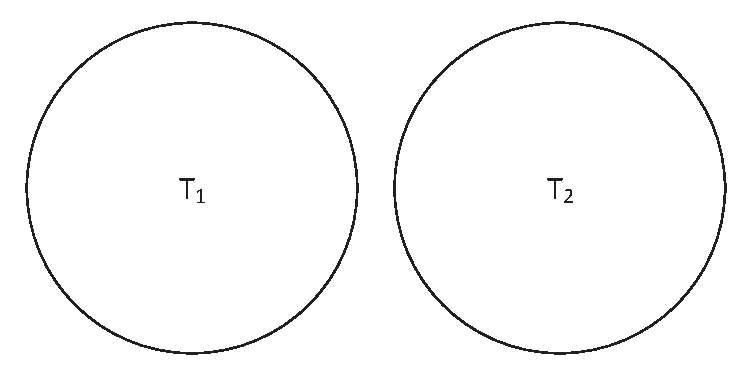
\includegraphics[width=2.01in]{testSuite2.eps}
}
\subfigure[]{
  %  \rule{4cm}{3cm}
    \label{fig:intersect}
    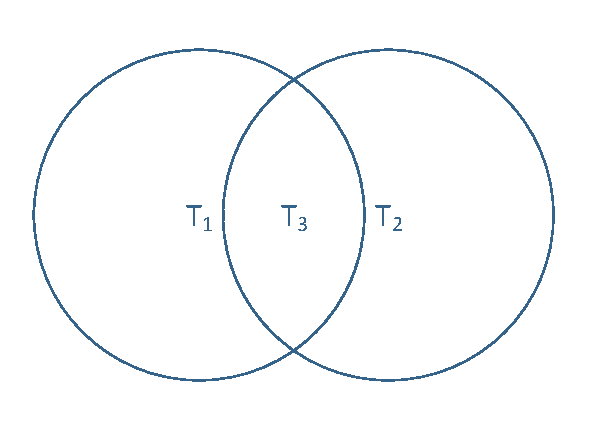
\includegraphics[width=1.81in]{testSuite3.eps}
}
\caption[]{Test suite relationships}
\label{fig:testSuite}
\end{figure*}

\subsection{Inclusion}

It is the first relationship corresponding to Figure \ref{fig:inclusion}. We can have the following proposition with two sets of test cases which have an inclusion relationship.
%\newtheorem{lemma}{Lemma}
\begin{proposition}[{schemas from smaller set tend to be parent schemas}]\label{pro:ssp}
For two sets of test cases $T_{l}$ and $T_{k}$, assume that $T_{l} \subset T_{k}$. Then for $ \forall c_{l} \in \mathcal{C}(T_{l})$ we have
 $\ either\ c_{l} \in \mathcal{C}(T_{k})\ or\ \exists c_{k} \in \mathcal{C}(T_{k}), s.t., c_{k} \prec c_{l}.$
\end{proposition}

\begin{proof}
Obviously for $\forall c_{l} \in \mathcal{C}(T_{l})$, we can get $\mathcal{T}(c_{l}) \subset T_{l} \subset T_{k}$. According to Proposition \ref{pro:sbS}, we can have $c_{l} \in \mathcal{S}(T_{k})$. So this proposition holds as the schema in $\mathcal{S}(T_{k})$ either is also in $\mathcal{C}(T_{k})$, or must be the parent of some schemas in $\mathcal{C}(T_{k})$.
\end{proof}

Likewise, we can get the properties of the schemas identified for the larger set of test cases.

\begin{proposition}[{schemas from larger set tend to be subschemas}]\label{pro:sls}
For two sets of test cases $T_{l}$ and $T_{k}$, assume that $T_{l} \subset T_{k}$. Then for $\forall c_{k} \in \mathcal{C}(T_{k})\ $ we have $either\ (1)\ c_{k} \in \mathcal{C}(T_{l})\ or\ (2)\ \exists c_{l} \in \mathcal{C}(T_{l}), s.t., c_{k} \prec c_{l}\ or\ (3)\ \not\exists c_{l} \in \mathcal{C}(T_{l}), s.t., c_{k} \prec c_{l}\ or\ c_{k} = c_{l},\ or\ c_{l} \prec c_{k}.$
% \begin{displaymath}
%  \begin{split}
%   either\ (1)\ c_{k} \in \mathcal{C}(T_{l})\\
%   or\ (2)\ \exists c_{l} \in \mathcal{C}(T_{l}), s.t., c_{k} \prec c_{l}\\
%   or\ (3)\ \not\exists c_{l} \in \mathcal{C}(T_{l}), s.t., c_{k} \prec c_{l}\ or\ c_{k} = c_{l},\ or\ c_{l} \prec c_{k}.
%  \end{split}
% \end{displaymath}
\end{proposition}

This proposition is exactly the antithesis of Proposition \ref{pro:ssp}. We need to note the third condition, i.e., $\ \not\exists c_{l} \in \mathcal{C}(T_{l}), s.t., c_{k} \prec c_{l}\ or\ c_{k} = c_{l},\ or\ c_{l} \prec c_{k}.$ We refer to this condition as $c_{k}$ is \emph{irrelevant} to $\mathcal{C}(T_{l})$. Furthermore, we can also say a schema is \emph{irrelevant} to another schema if these two schemas are neither identical nor subsuming each other.

%
%in fact, the schema $c_{k} \in \mathcal{C}(T_{k})$ remains with the following three possible relationships with $\mathcal{C}(T_{l})$ : (1) $c_{k} \in \mathcal{C}(T_{l})$, or (2) $\exists c_{l} \in \mathcal{C}(T_{l}), s.t.,\ c_{k} \prec c_{l}$, or (3) $\not\exists c_{l} \in \mathcal{C}(T_{l}), s.t., c_{k} \prec c_{l}\ or\ c_{k} = c_{l},\ or\ c_{l} \prec c_{k}$. For the third case, $c_{k}$ is called to be \emph{irrelevant} to $\mathcal{C}(T_{l})$.

We illustrate these scenarios in Table \ref{example_three_condition}. There are two parts in this table, with each part showing two sets of test cases: $T_{l}$ and $T_{k}$, which have $T_{l} \subset T_{k}$. For the left part, we can see that in the schema in $\mathcal{C}(T_{l})$: (0, 0, -) and (0, -, 0), both are the parent of the schema of the one in $\mathcal{C}(T_{k})$:(0,-,-). While for the right part, the schemas in $\mathcal{C}(T_{l})$: (0, 0, -) and (0, -, 0) are both also in $\mathcal{C}(T_{k})$. Furthermore, one schema in $\mathcal{C}(T_{k})$: (1,1,-) is irrelevant to $\mathcal{C}(T_{l})$.

%in which the left part shows the case that the failure-inducing combinations satisfy the first properties( both (0,0,-) and (0,1,0) subsume (0,-,-)). While the right part give an example to the second properties, as (1,-,-) is irrelevant to any one of (0,0,-) and (0,1,0).

%\begin{proof}
%We proof this by two sides:
%
%for there is one failure-inducing combination is this set, then this condition is similar to proposition 1, and For there is multiple failure-inducing combinations. We can easily find it must exist one failure-inducing combination.
%\end{proof}

\begin{table}
\centering
\tbl{Example of the scenarios\label{example_three_condition}}{
  \begin{tabular}{cc}
$T_{l}$&$T_{k}$ \\ \hline
(0, 0, 0)&(0, 0, 0)\\
(0, 0, 1)&(0, 0, 1) \\
(0, 1, 0)&(0, 1, 0)\\
         &(0, 1, 1) \\ \hline
 $\mathcal{C}(T_{l})$& $\mathcal{C}(T_{k})$ \\ \hline
(0, 0, -)&(0, -, -)\\
(0, -, 0)&		   \\ \hline
  \end{tabular}
  \hspace{1em}
  \begin{tabular}{cc}
$T_{l}$&$T_{k}$\\ \hline
(0, 0, 0) & (0, 0, 0)\\
(0, 0, 1) & (0, 0, 1)\\
(0, 1, 0) & (0, 1, 0)\\
		  & (1, 1, 0)\\
		  & (1, 1, 1)\\ \hline
$\mathcal{C}(T_{l})$& $\mathcal{C}(T_{k})$ \\ \hline
(0, 0, -)&  (0, 0, -)\\
(0, -, 0)&  (0, -, 0)\\
		 &  (1, 1, -)\\  \hline
  \end{tabular}
  }
  \end{table}

%It is noted that as the

\subsection{Disjoint}
This relationship corresponds to Figure \ref{fig:disjoint}. For two different sets of test cases, one obvious property is listed as follows:
\begin{proposition}[No relationships between the schemas]\label{pro:nrs}
 For two test cases set $T_{1}$,$T_{2}$, if $T_{1} \bigcap T_{2} = \emptyset $, we have, $\mathcal{S}(T_{1}) \bigcap \mathcal{S}(T_{2}) = \emptyset$.
\end{proposition}
\begin{proof}
 Assume that $\mathcal{S}(T_{1}) \bigcap \mathcal{S}(T_{2}) \ne \emptyset$. Without loss of generality, we let $c \in \mathcal{S}(T_{1}) \bigcap \mathcal{S}(T_{2}) $ we can learn that $\mathcal{T}(c)$ must both in $T_{1}$ and $T_{2}$, which is contradiction.
\end{proof}

This property tells that the minimal schemas of two disjointed test cases should be irrelevant to each other. Table \ref{example_disjoint} shows an example of this scenario. We can learn from this table that for two different test case sets $T_{l}$,$T_{k}$, their minimal schemas, i.e., (0, - , 0) and (1, 0, -),(1, -, 0), respectively, are irrelevant to each other.
\begin{table}
\centering
\tbl{Disjoint Example \label{example_disjoint}}{
  \begin{tabular}{cc}
$T_{l}$&$T_{k}$ \\ \hline
(0, 0, 0)&  (1, 0, 0)\\
(0, 1, 0)&  (1, 0, 1)\\
		 &  (1, 1, 0)\\  \hline
 $\mathcal{C}(T_{l})$& $\mathcal{C}(T_{k})$ \\ \hline
(0, -, 0)&(1, 0, -)\\
         &(1, -, 0)	\\ \hline
  \end{tabular}
  }
  \end{table}
%Sometimes they can be merged.

\subsection{Intersect}
This relationship corresponds to Figure \ref{fig:intersect}. This scenario is the most common scenario for two sets of test cases, but is also the most complicated scenario for analysis. To conveniently illustrate the properties of the minimal schemas of this scenario, we assume that $T_{1} \bigcap T_{2} = T_{3}$ as depicted in Figure \ref{fig:intersect}. Then, we can have the following properties:
%For two different set of test cases, one obvious properties is listed as follows:
%Without loss of generality, For $T_{1}$, their has three possibilities: $for c \in \mathcal{C}(T_{1})$, 1) $c \in  \mathcal{C}(T_{3})$, 2) $c \prec  \mathcal{C}(T_{3})$ 3) $c$ irrelevant to $\mathcal{C}(T_{3})$. This is also for $T_{2}$.

%Let me discuss the combination of them.
\begin{proposition}[Must have schemas that are irrelevant]\label{pro:mi}
 For two intersecting sets of test cases $T_{1}$ and $T_{2}$ (these two sets are neither identical nor do the members subsume each other), it must have $ \exists c_{1} \in \mathcal{C}(T_{1})\ and\ c_{2} \in \mathcal{C}(T_{2})$. s.t. $c_{1}\ and\ c_{2}$ are irrelevant.
\end{proposition}
\begin{proof}
First, we can learn that $\mathcal{C}(T_{1}\backslash T_{3})$ are irrelevant to $\mathcal{C}(T_{2} \backslash T_{3})$, as $(T_{1} \backslash T_{3}) \bigcap (T_{2} \backslash T_{3}) = \emptyset$.

As the schemas in $\mathcal{C}(T_{1} \backslash T_{3})$ are either identical to some schemas in $\mathcal{C}(T_{1})$ or parent schemas of them. Now, if some of them are identical, i.e., $\exists c', s.t., c' \in \mathcal{C}(T_{1} \backslash T_{3})\ and\  c' \in \mathcal{C}(T_{1})$, then schemas ${c'}$ must be irrelevant to these schemas in $ \mathcal{C}(T_{2})$ as $(T_{1} \backslash T_{3}) \bigcap T_{2} = \emptyset$. This also holds if $\mathcal{C}(T_{2} \backslash T_{3})$ is identical to some schemas in $\mathcal{C}(T_{2})$.

Next, if both $\mathcal{C}(T_{1} \backslash T_{3})$  and $\mathcal{C}(T_{2} \backslash T_{3})$ are parent schemas of some of $\mathcal{C}(T_{1})$ and $\mathcal{C}(T_{2})$, respectively. Without loss of generality, we let $c_{1} \prec c_{1-3}$, ($c_{1-3}\in\mathcal{C}(T_{1} \backslash T_{3})\ and\ c_{1} \in \mathcal{C}(T_{1})$) and $c_{2}\prec c_{2-3}$, ($c_{2-3}\in\mathcal{C}(T_{2} \backslash T_{3})\ and\ c_{2} \in \mathcal{C}(T_{2})$). Then, these corresponding sub-schemas in $\mathcal{C}(T_{1})$ and $\mathcal{C}(T_{2})$, i.e., $c_{1}$ and $c_{2}$ respectively, must also be irrelevant to each other. This is because $\mathcal{T}(c_{1}) \supset \mathcal{T}(c_{1-3})$ and  $\mathcal{T}(c_{2}) \supset \mathcal{T}(c_{1-3})$. And as $ \mathcal{T}(c_{1-3}) \bigcap  \mathcal{T}(c_{2-3}) = \emptyset $,  so $\mathcal{T}(c_{1})$ and $\mathcal{T}(c_{2})$ are neither identical nor subsuming each other. This also implies that $c_{1}$ and $c_{2}$ are irrelevant to each other.
\end{proof}

For example, Table \ref{example_intersect_irrelevant} shows two test cases that interact with each other at test case (1,0,0), but their minimal schemas, (1,0,-) and (1,-,0), respectively, are irrelevant to each other.

\begin{table}
\centering
\tbl{Example of Intersection by irrelevant examples \label{example_intersect_irrelevant}}{
  \begin{tabular}{cc}
$T_{1}$&$T_{2}$ \\ \hline
(1, 0, 0) &  (1, 0, 0)\\
(1, 0, 1) &  (1, 1, 0)\\  \hline
 $\mathcal{C}(T_{1})$& $\mathcal{C}(T_{2})$ \\ \hline
(1, 0, -)&(1, -, 0)\\
  \end{tabular}
  }
  \end{table}

\begin{proposition}[Can be identical]\label{pro:ci}
 For two intersecting sets of test cases $T_{1}$ and $T_{2}$, and let $T_{3} = T_{1} \bigcap T_{2}$, if $\exists c_{1} \in \mathcal{C}(T_{1})\ and\ c_{2} \in \mathcal{C}(T_{2})$ which are identical, then it must have $c_{1} = c_{2} \in \mathcal{C}(T_{3})$
\end{proposition}
\begin{proof}
As we see that identical schemas must have the same set of test cases that contain them, then the only same set of test cases between $T_{1}$ and $T_{2}$ is $T_{1} \bigcap T_{2} = T_{3}$. So the only possible identical schema between $\mathcal{C}(T_{1})$ and $\mathcal{C}(T_{2})$ is in $\mathcal{C}(T_{3})$.
\end{proof}

We must know that this proposition holds when some schemas in $\mathcal{C}(T_{1} \bigcap T_{2})$ are identical to some schemas in $\mathcal{C}(T_{1})$ and $\mathcal{C}(T_{2})$.

For example, Table \ref{example_intersect_identical} shows two test cases that interact with each other at test cases (1,1,0) and (1,1,1), and they have identical minimal schema, i.e., (1,1,-), which is also the minimal schema in $\mathcal{C}(T_{3})$.

\begin{table}
\centering
\tbl{Example of Intersection by identical examples \label{example_intersect_identical}}{
  \begin{tabular}{ccc}
$T_{1}$&$T_{2}$ &$T_{3} = T_{1} \bigcap T_{2}$\\ \hline
 (0, 1, 0) & (0, 0, 0) & (1, 1, 0) \\
 (1, 1, 0) & (0, 0, 1) & (1, 1, 1)\\
 (1, 1, 1) & (1, 1, 0) & \\
	       & (1, 1, 1) & \\\hline

 $\mathcal{C}(T_{1})$& $\mathcal{C}(T_{2})$ & $\mathcal{C}(T_{3})$  \\ \hline
(-, 1, 0)&  (0, 0, -) & (1, 1, -)\\
(1, 1, -)&  (1, 1, -) &\\ \hline
  \end{tabular}
  }
  \end{table}

%It must also be that this $c$ must in $T_{3}$, which means that it should not all be children tuples like table.

\begin{proposition}[Can be subsuming each other]\label{pro:cs}
 For two intersecting sets of test cases $T_{1}$ and $T_{2}$, let $T_{3} = T_{1} \bigcap T_{2}$, if  $\exists c_{1} \in \mathcal{C}(T_{1})\ and\ c_{2} \in \mathcal{C}(T_{2})$, which satisfy that $c_{1}$ is the parent-schema of $c_{2}$, then it must have $c_{1} \in \mathcal{C}(T_{3})$. (and vice versa).
\end{proposition}
\begin{proof}
We have proved previously if two schemas have have a subsuming relationship, then their test cases must also have an inclusion relationship. And as the only inclusion relationship between  $T_{1}$ and $T_{2}$ is that $ T_{3} \subset  T_{1}  $  and $T_{3}\subset  T_{2}$. So the parent schemas must be in $\mathcal{C}(T_{3})$.
\end{proof}

It is noted that this proposition holds when some schemas in $\mathcal{C}(T_{3})$ are also in $\mathcal{C}(T_{1})$ (or $\mathcal{C}(T_{2})$), and simultaneously the same schemas in $\mathcal{C}(T_{3})$ must be the parent-schema of the minimal schemas of another set of test cases, i.e., $\mathcal{C}(T_{2})$ (or $\mathcal{C}(T_{1})$).

Table \ref{example_intersect_subsume} illustrates this scenario, in which, the minimal schemas of $T_{1}$: (1,0,-),(1,-,0),which are also the schemas in $\mathcal{C}(T_{3})$, is the parent schema of the minimal schema of $T_{2}$: (1,-,-).

\begin{table}
\centering
\tbl{Example of Intersect by subsuming examples \label{example_intersect_subsume}}{
  \begin{tabular}{ccc}
$T_{1}$&$T_{2}$ &$T_{3}  = T_{1} \bigcap T_{2} $\\ \hline
(0, 1, 0)   & (0, 0, 0) & (1, 0, 0) \\
(1, 0, 0)   & (1, 0, 0) & (1, 0, 1)\\
(1, 0, 1)	& (1, 0, 1) & (1, 1, 0)\\
(1, 1, 0)	& (1, 1, 0) &         \\
        	& (1, 1, 1) & \\ \hline
 $\mathcal{C}(T_{1})$& $\mathcal{C}(T_{2})$ & $\mathcal{C}(T_{3})$  \\ \hline
(-, 1, 0)&  (-, 0, 0) & (1, 0, -)\\
(1, 0, -)&  (1, -, -) & (1, -, 0)   \\
(1, -, 0)&     & \\ \hline
  \end{tabular}
  }
  \end{table}

 It is noted that these three conditions can simultaneously appears when two sets of test cases intersect with each other.%, like Table \ref{example_intersect_all}.
%\begin{table}
%\centering
%\tbl{Example of Intersect by all examples \label{example_intersect_all}}{
%  \begin{tabular}{ccc}
%$T_{1}$&$T_{2}$ &$T_{3}$\\ \hline
%(0, 1, 0)   & (0, 0, 0) & (1, 0, 0) \\
%(1, 0, 0)   & (0, 0, 1) & (1, 0, 1)\\
%(1, 0, 1)	& (1, 0, 0) & (1, 1, 0)\\
%(1, 1, 0)	& (1, 0, 1) &         \\
%        	& (1, 1, 0)\\
%		    & (1, 1, 1)\\ \hline
% $\mathcal{C}(T_{1})$& $\mathcal{C}(T_{2})$ & $\mathcal{C}(T_{3})$  \\ \hline
%(0, 1, 0)&  (0, 0, -) & (1, 0, -)\\
%(1, 0, -)&  (1, -, -) & (1, -, 0)   \\
% (1, -, 0) & & \\ \hline
%  \end{tabular}
%  }
%  \end{table}

%\subsection{Summary of the formal model}
%From the previous analysis, we can learn that for the general intersect test cases-schema model, this is a partial relationship.

\subsection{Identify the MFS}
According to this analysis, we can determine that $\mathcal{C}(T_{F_{m}})$ actually is the set of failure-causing schemas of $F_{m}$. Then in theory, if we want to accurately figure out the MFS in the SUT, we need to exhaustively execute each possible test case, and collect the failing test cases $T_{F_{m}}$. This is impossible in practice, especially when the testing space is very large.

So for traditional FCI approaches, they need to select a subset of the exhaustive test cases, and then either use some assumptions to predict the remaining test cases or just give a suspicious ranking. As giving a suspicious ranking can also be regard as a special case of making a prediction (with computing the possibility), so we next only formally describe the mechanism of FCI approaches belonging to the first type.
%Formally, we can describe the two ways as following:
We refer to the observed failing test case as  $T_{fail_{observed}}$, and refer to the remaining failing test cases based on prediction as $T_{fail_{predicted}}$. We also denote the actual entire failing test cases as $T_{fail}$. Then the MFS identified by FCI approaches can be depicted as:

MFS = $\mathcal{C}(T_{fail_{observed}} \bigcup T_{fail_{predicted}})$.

For each FCI approach, the way it predicts the $T_{fail_{predicted}}$ according to observed failing test cases varies; furthermore, as the test cases it generates are different, the failing test cases observed by different FCI approaches, i.e., $T_{fail_{observed}}$ also varies.  We offer an example using the OFOT approach to illustrate this formula.

Suppose that the SUT has 3 parameters, each of which can take 2 values. And assume the test case (1, 1, 1) failed. Then, we can describe the FCI process as shown in Table \ref{ofot-identify}. In this table, test case \emph{t} failed, and OFOT mutated one parameter value of the test case \emph{t} at a time to generate new test cases: $t_{1}; t_{2}; t_{3}$, It found the $t_{1}$ passed, which indicates that this test case breaks the MFS in the original test case \emph{t}. So, the (1,-,-) should be one failure-causing factor, and as the other test cases ($t_{2}, t_{3}$) all failed , this means no other failure-inducing factors were broken; therefore, the MFS in \emph{t} is (1,-,-).

Now let us explain this process with our formal model. Obviously the $T_{fail_{observed}}$ is \{(1,1,1),(1,0,1),(1,1,0)\}. And as having found (0,-,-) broke the MFS, hence by theory\cite{nie2011minimal}, all the test cases that contain (0,-,-) should pass the testing (This conclusion is built on the assumption that the SUT just contain one failure-causing schema).  As a result, {(0,1,1),(0,0,1),(0,1,0),(0,0,0)} should pass the testing. Further, as obviously the test case either passes or fails (the condition that a test case skips testing, i.e., doesn't produce an output, is labeled as a special case of failing), so the remaining test case(1,0,0), will be predicted to be failing, i.e., $T_{fail_{predicted}}$ is \{(1,0,0)\}. Taken together, the MFS using the OFOT strategy can be described as: $\mathcal{C}(T_{fail_{observed}} \bigcup T_{fail_{predicted}})$ = $\mathcal{C}(\{(1,1,1),(1,0,1),(1,1,0),(1,0,0)\})$ = (1,-,-), which is identical to the one that was gotten previously.

\begin{table}[h]
\tbl{OFOT with our strategy\label{ofot-identify}}{
\begin{tabular}{llllll}
\multicolumn{5}{c}{\bfseries original test case} & \bfseries Outcome \\
 $t$ & \multicolumn{4}{l}{1 \ \ \ \ 1 \ \ \ \  1 } & Fail \\
 \hline
\multicolumn{5}{c}{\bfseries observed} &  \\
$t_{1}$ &\multicolumn{4}{l}{0  \ \ \ \  1 \ \ \ \  1 }& Pass \\
$t_{2}$ &\multicolumn{4}{l}{1  \ \ \ \  0 \ \ \ \  1 } & Fail \\
$t_{3}$ &\multicolumn{4}{l}{1  \ \ \ \  1 \ \ \ \  0 } & Fail \\
\hline
\multicolumn{5}{c}{\bfseries predicted} & \\
$t_{4}$ &\multicolumn{4}{l}{0  \ \ \ \  0 \ \ \ \  1 } & Pass \\
$t_{5}$ &\multicolumn{4}{l}{0  \ \ \ \  1 \ \ \ \  0 } & Pass \\
$t_{6}$ &\multicolumn{4}{l}{1  \ \ \ \  0 \ \ \ \  0 } & Fail \\
$t_{7}$ &\multicolumn{4}{l}{0  \ \ \ \  0 \ \ \ \  0 } & Pass \\
\end{tabular}}
\end{table}
%In this formula, the approach can derive the $T_{fail_{assumed}}$ from the $T_{fail_{observed}}$. For example,  for OFOT, one factor, pass, it can learn all the factor. For colbourn, it can learn from the covering array to be all according the number and t.


\begin{figure}
\centering
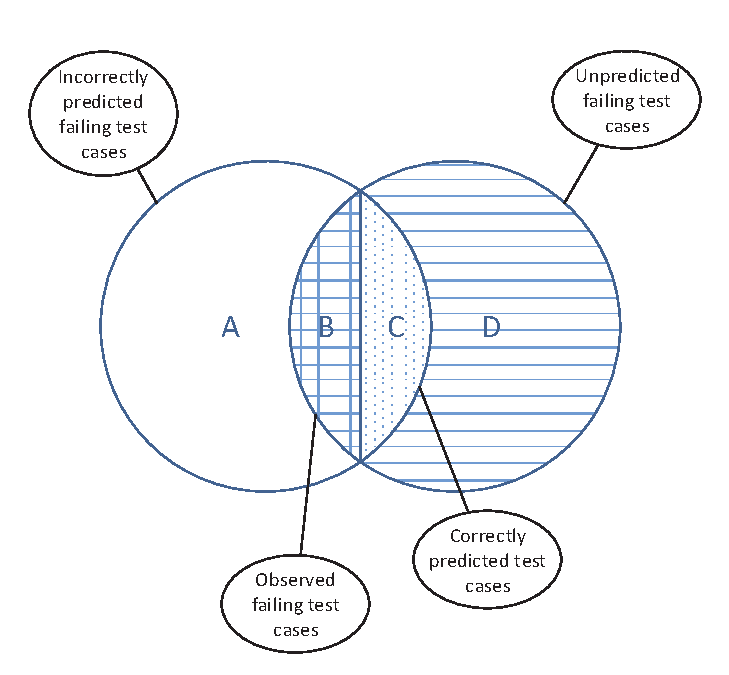
\includegraphics[width=3.31in]{FCI.eps}
\caption{Generally model of FCI}
\label{fig:fci_process}
\end{figure}

Similarly, other FCI approaches can also be modeled into this formal description. We will not discuss in detail how to model each FCI approach as this is not the point of this paper. It is noted that the test cases FCI predicts to be failing are not always identical to the actually failing test cases. In fact, we can generally depict the process of FCI approaches as shown in Figure \ref{fig:fci_process}.

We can see in Figure \ref{fig:fci_process} that area A denotes the test cases that should have passed testing but were predicted to be failing, area B depicts the test cases that the approach observed to be failing test cases, area C refers to the failing test cases that were not observed to be but were predicted to be failing test cases, and area D shows the failing test cases that are neither observed nor predicted.  This figure actually represents the condition in which two sets of test cases intersect with each other; in specific, comparing to the Figure \ref{fig:intersect}, we can learn areas $A \bigcup B \bigcup C $= $T_{1}$,  $D \bigcup B \bigcup C $= $T_{2}$ and $ B \bigcup C$ = $ T_{1} \bigcap T_{2} = T_{3}$.

As we have known, in the case of Figure \ref{fig:intersect}, there are various relationships between the schemas identified in $T_{1}$ and the schemas identified in $T_{2}$. According to Proposition \ref{pro:mi}, some schemas in $\mathcal{C}(T_{1})$ and in $\mathcal{C}(T_{2})$ must be irrelevant to each other. Mapping to Figure \ref{fig:fci_process}, we can get that some schemas in $\mathcal{C}(A \bigcup B \bigcup C)$ and in $\mathcal{C}(D \bigcup B \bigcup C)$ must be irrelevant to each other, which means that the FCI approach will identify some minimal schemas that are irrelevant to the actual MFS, and must ignore some actual MFS. Moreover, under the appropriate conditions listed in Propositions \ref{pro:ci} and \ref{pro:cs}, FCI may identify the identical schemas or parent-schema or sub-schema of the actual MFS. In this case, the schemas (those identical ones, parent-schemas, or sub-schemas) are all depended on the area $B \bigcup C$, namely $T_{1} \bigcap T_{2}$ in Figure \ref{fig:intersect}. So to identify the schemas as accurately as possible, the FCI approach needs to make $A \bigcup B \bigcup C$ as similar as possible to $D \bigcup B \bigcup C$.

However, even though each FCI approach tries its best to identify the MFS as accurately as possible, masking effects raised from the test cases will result in their efforts being in vain. We next will discuss the masking problem and how it affects the FCI approaches.

%Thus, besides the case that FCI make a perfect prediction, $T_{fail_{observed}} \bigcup T_{fail_{predicted}}$ can either contain $T_{fail}$ or be contained by $T_{fail}$ , or neither of the two circumstances. For the third circumstance, we have the following proposition:
%
%\begin{proposition}
% If neither $T_{m} \subset T_{n}$ nor $T_{n} \subset T_{m}$, then it must be that $c \in $ $\mathcal{C}(T_{n}) $ is irrelevant to $\mathcal{C}(T_{m})$ and must be some $c' \in $ $\mathcal{C}(T_{m}) $ is irrelevant to $\mathcal{C}(T_{n})$  .
%\end{proposition}
%
%\begin{proof}
%We just need to prove the first one, as the latter is equivalent to the first one. The first one can be proven by contradiction.
%
%Assume that for $\forall c \in \mathcal{C}(T_{m})$, have $c either \in \mathcal{C}(T_{n}) $.
%\end{proof}
%
%So either of this three circumstance can make FCI identifying inaccurately as we discussed earlier, and each FCI should avoid these circumstances as much as possible.

%\subsubsection{Proposition of MFS identifying process}

%\subsubsection{Suspicious}
%SP, CTA. The first one will, while the latter not.

%\subsection{Discussion of the formal model}
%This section gives a formal analysis of the CT testing and diagnosis model. In specific, we gave the definitions of the SUT model and proposed the possible relationships between the schemas and the set of test cases that contained them. Based on this we defined a general MFS identifying model.
%
%It is noted that, at the beginning of this section, we have mentioned two assumptions. Now we will discuss some probable impacts of them on the MFS identifying process and give some to .
%
%The first one assumes that the outcome of the execution of a test case is deterministic. When the software is indeterministic, i.e., tests that sometimes pass and sometimes fail, we may totally get wrong results if we just identify the MFS one time without any more actions. then
% multiple runs, and get these
%
%The second,  different failures cannot be distinguished.

\section{Masking effect}
\begin{definition}
A \emph{masking effect} is an effect that when a test case \emph{t} contains an MFS for a particular failure, but the test case $t$ does not trigger the expected failure because another failure was triggered ahead of it that prevents $t$ from being normally checked.
\end{definition}

Taking the masking effects into account, when identifying the MFS for a specific failure, say, $F_{m}$, we should not ignore these test cases which did not trigger $F_{m}$ but should have triggered it. We call these test cases $T_{mask(F_{m})}$. Hence, the MFS for failure $F_{m}$ should be $\mathcal{C}(T_{F_{m}} \bigcup T_{mask(F_{m})})$.

As an example, in the motivation example in section 2, the $F_{mask(F_{Ex\ 2})}$  is \{ (7,4,4,5),(11,4,4,5)\}, So the MFS for $Ex 2$ is $\mathcal{C}(T_{F_{Ex\ 2}} \bigcup T_{mask(F_{Ex\ 2})})$, which is (-,-,4,5).

In practice with masking effects, however, it is not possible to correctly identifying the MFS, unless we fix some bugs in the SUT and re-execute the test cases to figure out $T_{mask(F_{m})}$.

In effect for traditional FCI approaches, without the knowledge of  $T_{mask(F_{m})}$,  only two strategies can be adopted when facing the multiple failures problem. We will separately analyse the two strategies under exhaustive testing condition and normal FCI testing condition.
\subsection{Masking effects for exhaustive testing}

\subsubsection{Regarded as one failure}
The first is the most common strategy, as it does not distinguish the failures, i.e., it treats all of the types of failures as one failure--\emph{failure}, and others as \emph{pass}.

With this strategy, the minimal schemas we identify are the set $\mathcal{C}(\bigcup_{i = 1}^{L}T_{F_{i}})$ , $L$ is the number of all the failures in the SUT. Obviously, $T_{F_{m}} \bigcup T_{mask(F_{m})} \subset \bigcup_{i = 1}^{L}T_{F_{i}}$ . So in this case, by Proposition \ref{pro:sls}, some schemas we get may be the sub-schemas of some of the actual MFS, or be irrelevant to the actual MFS.

As an example, consider the test cases in Table \ref{masking-effects-exhaustive}. In this example, assume we need to characterize the MFS for error \emph{1}. All the test cases that triggered error 1 are listed in column \emph{$T_{1}$}; similarly, we list the test cases that triggered other failures in column \emph{$T_{mask(1)}$} and \emph{$T_{*}$}, respectively, in which the former masked the error 1, while the latter did not. Actually the MFS for error 1 should be (1,1,-,-) and (-,1,1,1) as we listed them in the column \emph{actual MFS for 1}. However, when we use the \emph{regarded as one failure} strategy, the minimal schemas we get will be (-,-,0,0), (1,1,-,-), (-,-,1,1), in which the (-,-,0,0) is irrelevant to the actual MFS for error 1, and the (-,-,1,1) is the sub-schema of the actual MFS (-,1,1,1).

\begin{table}
\centering
\tbl{masking effects for exhaustive testing \label{masking-effects-exhaustive}}{
  \begin{tabular}{ccc}
$T_{1}$&$T_{mask(1)}$ &$T_{*}$\\ \hline
(1, 1, 1, 1)& (1, 1, 0, 0) & (0, 1, 0, 0) \\
(1, 1, 1, 0)& (0, 1, 1, 1) & (0, 0, 0, 0)\\
(1, 1, 0, 1)&              & (1, 0, 0, 0)\\
          	&              & (1, 0, 1, 1)\\
        	&              & (0, 0, 1, 1)\\ \hline
actual MFS for 1&  regarded as one failure & distinguishing failures  \\
$\mathcal{C}(T_{1}  \bigcup T_{mask(1)})$& $\mathcal{C}(T_{1}  \bigcup T_{mask(1)}  \bigcup T_{*})$ & $\mathcal{C}(T_{1})$  \\ \hline
(1, 1, -, -)&  (-, -, 0, 0) & (1, 1, -, 1)\\
(-, 1, 1, 1)&  (1, 1, -, -) & (1, 1, 1, -)   \\
            &  (-, -, 1, 1) &         \\ \hline
  \end{tabular}
  }
  \end{table}

\subsubsection{Distinguishing failures}
Distinguishing the failures by the exception traces or error code can help make the MFS related to particular failure. Yilmaz \cite{yilmaz2013reducing} proposed the \emph{multiple-class} failure characterizing method instead of the \emph{ternary-class} approach to make the characterizing process more accurate. Besides, other approaches can also be easily extended with this strategy for testing SUT with multiple failures.
%We call this strategy \emph{distinguishing failures}.

This strategy focuses on identifying the set of $\mathcal{C}(T_{F_{m}})$, and as $T_{F_{m}} \bigcup T_{mask(F_{m})} \supset T_{F_{m}} $, consequently, some schemas that get through this strategy may be the parent-schema of some actual MFS. Moreover, some MFS may be irrelevant to the schemas we get with this strategy, which means this strategy will ignore these actual MFS.

For the simple example in Table \ref{masking-effects-exhaustive}, when we use this strategy, we will get the minimal schemas (1, 1, -, 1) and (1, 1, 1, -), which are both the parent schemas of the actual MFS (1,1,-,-), and we will observe that no schemas gotten by this strategy have any relationship with the actual MFS (-,1,1,1), which means it was ignored.

It is noted that the motivation example in section 2 actually adopted this strategy, so we see that the schemas identified for Ex 2: (-,2,4,5), (-,3,4,5) are the parent-schemas of the correct MFS(-,-,4,5).

\subsection{Masking effects for FCI approaches}
With masking effects, the scenario of traditional FCI approaches is a bit more complicated than the previous two exhaustive testing scenarios, and is depicted in Figure \ref{fig:fci_mask}. In this figure,  areas A, C and D are the same as in Figure \ref{fig:fci_process}, and area B is divided into three sub-areas in which $B_{1}$ still represents the observed failing test cases for the current analysed failure, area $B_{2}$ represents the test cases that triggered other failures which masked the current failure, and area $B_{3}$ represents the test cases that triggered other failures which did not mask the current failure. It can be found that the actual MFS set for the SUT is $\mathcal{C}(B_{1} \bigcup B_{2} \bigcup C \bigcup D)$.

\begin{figure}
\centering
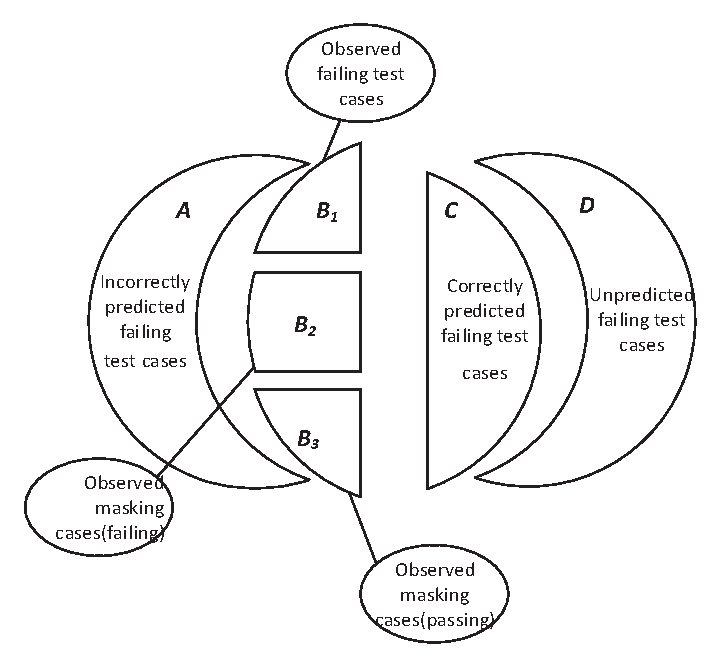
\includegraphics[width=3.31in]{FCI-mask.eps}
\caption{FCI with masking effects}
\label{fig:fci_mask}
\end{figure}

With this model, if we know which test cases mask the expected failure, i.e., if we have figured out the B2 and B3 areas, then the schemas that the FCI approach will identify can be described as $\mathcal{C}(A \bigcup B_{1} \bigcup B_{2} \bigcup C)$.  We next denote the condition that we have known the masking effects in prior as \emph{knowing masking effects}. However, as we discussed before, to get this result is not possible without human involvement. Correspondingly, when using the \emph{regarded as one failure} strategy, the set of MFS traditional FCI identify is $\mathcal{C}(A \bigcup B_{1} \bigcup B_{2} \bigcup B_{3} \bigcup C)$.  And for the \emph{distinguishing failures} strategy, the MFS is $\mathcal{C}(A \bigcup B_{1} \bigcup C)$. Next, we will discuss the influence of masking effects on the two strategies.

\subsubsection{Using the regarded as one failure strategy}

For the first strategy: \emph{regarded as one failure}, the impact of masking effects on FCI approaches can be described as shown in Table \ref{fci_mask_regard}. To understand the content of this table, let us go back to the relationship between the minimal schemas of two different sets of test cases. For the \emph{knowing masking effects} condition, the test cases that are used for identifying the MFS, i.e., $A \bigcup B_{1} \bigcup B_{2} \bigcup C $, \emph{intersect} the test cases that are used to compute the actual MFS( $ B_{1} \bigcup B_{2} \bigcup C \bigcup D$ ). It means that the minimal schemas get in this condition can be identical, parent-schema, sub-schema, and irrelevant to the actual MFS. And if we apply the \emph{regarded as one failure}, the minimal schemas we get are $\mathcal{C}(A \bigcup B_{1} \bigcup B_{2} \bigcup B_{3} \bigcup C)$. Obviously, we have $A \bigcup B_{1} \bigcup B_{2} \bigcup B_{3} \bigcup C$ $\supset$ $A \bigcup B_{1} \bigcup B_{2} \bigcup C$. So the minimal schema gotten by this strategy is either the sub-schema or identical to some schemas from the ones gotten by \emph{known masking effects}, or alternatively, existing some schemas that are irrelevant to all of them. Taking these two properties together, we will get what is shown in Table \ref{fci_mask_regard}.

%\begin{figure}
%\centering
%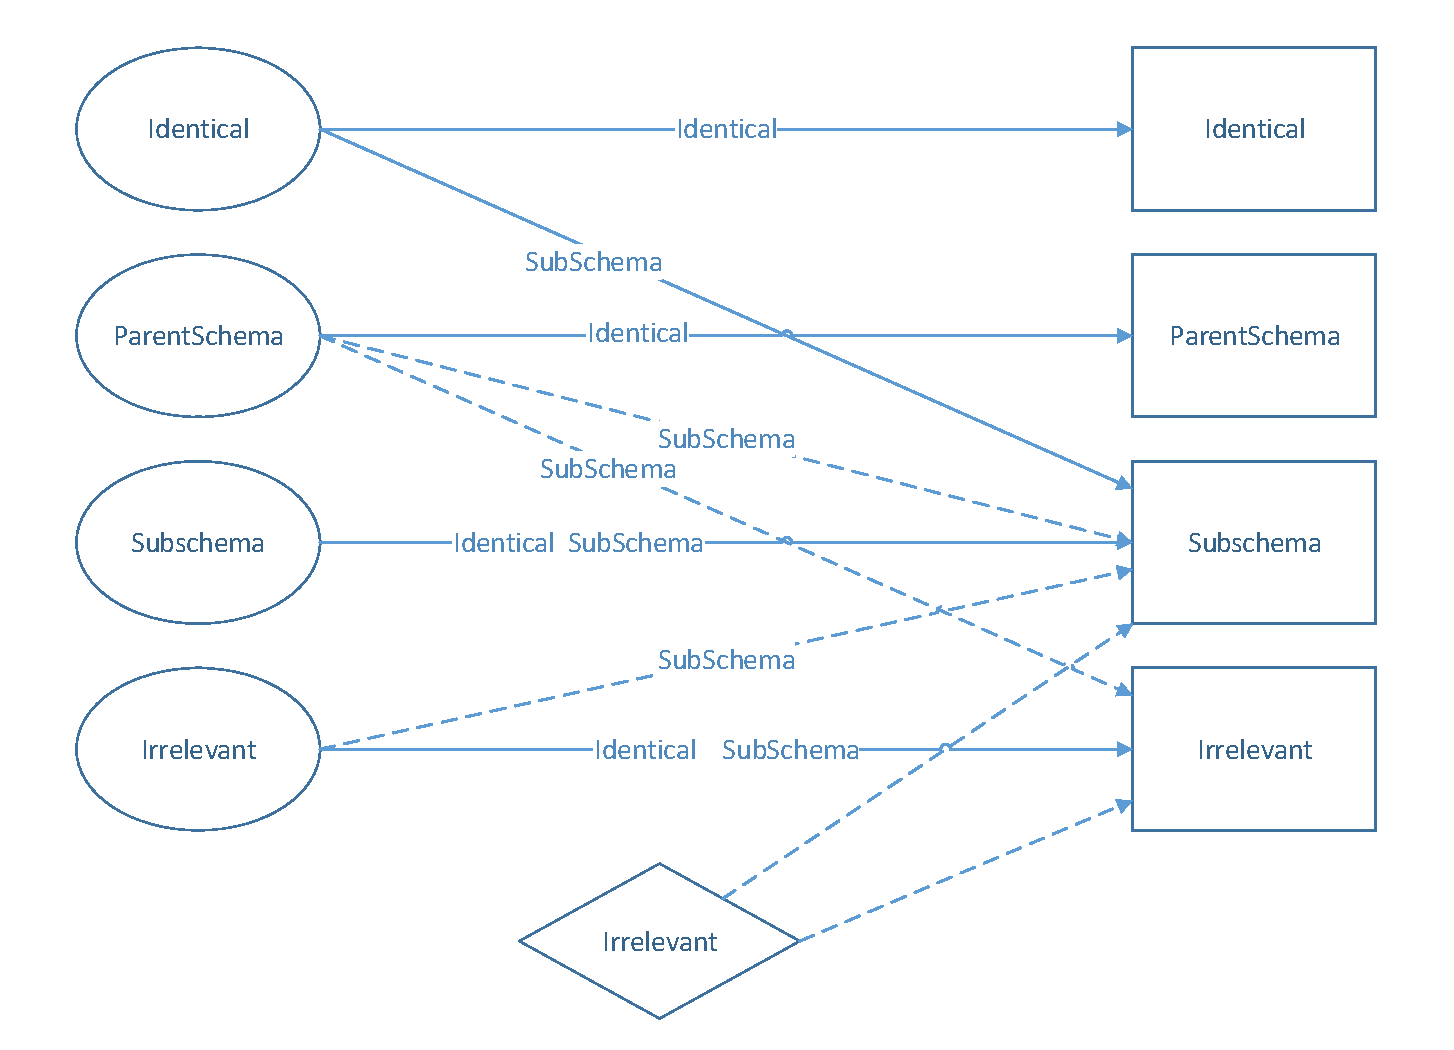
\includegraphics[width=4.31in]{fci-mask-influence2.eps}
%\caption{Masking effects influence on FCI with regarded as one failure}
%\label{fig:fci_mask_regard}
%\end{figure}

\begin{table}[h]
\tbl{Masking effects influence on FCI with regarded as one failure strategy
\label{fci_mask_regard}}{
\begin{tabular}{|lll|}
\hline
1  & If  $ c_{m} = c_{origin}$ \  and\   $c_{new} = c_{origin}  $                                & Then, $ \exists c_{m}',s.t.,c_{new} = c_{m}'  $             \\
2  &  If  $ c_{m} = c_{origin}$   and\   $c_{new} \prec c_{origin} $       & Then,  $\exists c_{m}',s.t.,c_{new} \prec c_{m}'  $              \\
3  & If $c_{m} \prec c_{origin}$\ and\  $c_{new} = c_{origin}  $                 & Then, $\exists c_{m}',s.t.,c_{m}' \prec c_{new} $               \\
4a & If $c_{m} \prec c_{origin}$\  and\ $c_{new} \prec c_{origin}$                 & Then either,$c_{m}',s.t.,c_{new} \prec c_{m}' $        \\
4b &                                                                     & Or,$ c_{new}\ irrelevant\ to\ all\ c_{m}'  $ \\ %\hline
5  & If $c_{origin} \prec c_{m}$\ and\ $c_{new} = c_{origin}  $          & Then, $\exists c_{m}',s.t.,c_{new} \prec c_{m}' $               \\
6  & If $c_{origin} \prec c_{m}$\  and\ $c_{new} \prec c_{origin} $      & Then, $\exists  c_{m}',s.t.,c_{new} \prec c_{m}'  $              \\ %\hline
7  & If $c_{origin}\ irrelevant\ all\ c_{m}$\ and\ $c_{new} = c_{origin} $                  & Then, $ c_{new}\ irrelevant\ to\ all\ c_{m}'$ \\
8a & If $c_{origin}\ irrelevant\ all\ c_{m}$\ and\ $c_{new} \prec c_{origin}$     & Then either,$\exists c_{m}',s.t.,c_{new} \prec c_{m}'$         \\
8b &                                                                                      & Or,$c_{new}\ irrelevant\ to\ all\ c_{m}'  $ \\ %\hline
9a &            If $c_{new}\ irrelevant\ to\ all\ c_{origin}$ & Then either,$\exists c_{m}',s.t.,c_{new} \prec c_{m}' $        \\
9b &                                                             & Or,$ c_{new}\ irrelevant\ to\ all\ c_{m}' $  \\ \hline
\end{tabular}}
\end{table}

There are totally 9 rules for this strategy, which are labeled from 1 to 9 respectively. In these rules, $c_{m}$ and $c_{m}'$ are the actual MFSs, i.e., $c_{m}, c_{m}' \in C(B_{1} \bigcup B_{2} \bigcup C \bigcup D)$. $c_{origin}$ is the minima schema that are gotten by \emph{knowing masking effects} strategy, i.e., $c_{origin} \in \mathcal{C}(A \bigcup B_{1} \bigcup B_{2} \bigcup C)$. $c_{new}$ is the schema that are gotten by \emph{regarded as one failure} strategy, i.e., $c_{new} \in \mathcal{C}(A \bigcup B_{1} \bigcup B_{2} \bigcup B_{3} \bigcup C)$. $c_{new}$ satisfies that $c_{new} = c_{origin}$ or $c_{new} \prec c_{origin}$.  Each rule in Table \ref{fci_mask_regard}  describes one possible relationship between the schemas gotten by strategy \emph{regarded as one failure} and the actual MFS. For example,
rule 2, i.e., $If\ c_{m} = c_{origin}\ and\ c_{new} \prec c_{origin}, then\ \exists c_{m}', s.t., c_{new} \prec c_{m}'$, indicates that the schema $c_{new}$ that is gotten by \emph{regarded as one failure} strategy will be the subschema of some actual MFS, if it is the subschema of the schema $c_{origin}$ that is gotten by strategy \emph{knowing masking effects}, and $c_{origin}$ is identical to some actual MFS. Some rules may result in that there are more than one possible relationship between the $c_{new}$ and the actual MFS. For example, rule 4 can make $c_{new}$ either be the subschema of the actual MFS or be irrelevant to all the actual MFS. In this case, we divide the rule into several sub-rules. As for rule 4 we divide this rule into two sub-rules: 4a and 4b, each of which represents one possibility relationship between the $c_{new}$ and the actual MFS $c_{m}'$.

In these rules, only two can make $\exists c_{m}', s.t.$ $c_{new} = c_{m}'$ or $c_{m}' \prec c_{new}$, which are rules 1 and 3 respectively. This can be easily understood, as to make  $c_{new} = c_{m}'$ or $c_{m}' \prec c_{new}$, according to Proposition \ref{pro:ci} and \ref{pro:cs}, it must have $\mathcal{T}(c_{new}) \subset (B_{1} \bigcup B_{2})$. Assume we get $c_{new} \prec c_{origin}$, then we must have $\exists t \in B_{3}, s.t., t \in \mathcal{T}(c_{new})$, otherwise, there should be no schema $c_{new}$ that is the sub-schema of $c_{origin}$. Consequently, $\mathcal{T}(c_{new}) \not\subset (B_{1} \bigcup B_{2})$ if we have $c_{new} \prec c_{origin}$. So to make $c_{new} = c_{m}'$ or $c_{m}' \prec c_{new}$, the schema $c_{new}$ must be identical to $c_{origin}$, i.e., $c_{new} = c_{origin}$ and there must be $c_{origin} = c_{m}$ or $c_{m} \prec c_{origin}$, correspondingly. Apart from these two rules, the remaining rules indicate that either $c_{new} \prec c_{m}'$ or $c_{new}\ is\ irrelevant\ to\ all\ the\ actual\ MFS$, which implies the schemas that are gotten by strategy \emph{regarded as one failure} tends to be more subschemas or irrelevant schemas of the actual MFS when compared to that of the \emph{knowing masking effects} strategy.

% and is identical to some actual MFS, and the schema gotten by \emph{regarded as one failure} is the subschema of the .  Some rules can be divided into two parts. For example,
%
%When the that, ie,

%The ellipses in the left column of this figure illustrate the relationship between the schemas identified under the \emph{knowing masking effects} condition with the actual MFS, which includes the four possibilities: identical, sub-schema, parent-schema and irrelevant. For each relationship in this part, without of loss of generality, we consider $c_{origin}$ and $c_{m}$. $c_{origin}$ is the minima schema gotten by \emph{knowing masking effects}, and $c_{m}$ is the actual MFS. Then, when we apply the \emph{regarded as one failure} strategy, we may get some schemas which are identical or sub-schema of $c_{origin}$, say $c_{new}$ s.t., $c_{new} = c_{origin}$ or $c_{new} \prec c_{origin}$. In this figure, we use the directed line to represent these two transformations with different labels in each line. As for the schemas $c_{new}$ that are irrelevant to all the $c_{origin}$, we in the bottom of this figure use a rhombus labeled "Irrelevant" to represent them. Then, we must have some relationship between the $c_{new}$ and actual MFS, which also has four possibilities represented as rectangles in the right column.

%Note that there exist two types of directed line -- solid line and dashed line, in which the former indicates that this transformation is deterministic, e.g., if $c_{origin} \prec c_{m}$ and $c_{new} \prec c_{origin}$, then we must have $c_{new} \prec c_{m}$.  The latter type means the transformation is just one of all the possibilities in such condition, e.g., if $c_{origin}\ irrelevant\ c_{m}$ and $c_{new} \prec c_{origin}$, then we can have either $\exists c_{m}'\ is\ one\ actual\ MFS, s.t. c_{new} \prec c_{m}$ or $c_{new}\ irrelevant \ to\ all\ actual\ MFS$. (We will later give illustrative examples.)

%In this figure, only two transformations can make $\exists c_{m}'\ is\ one\ actual\ MFS, s.t.$ $c_{new} = c_{m}'$ or $c_{m}' \prec c_{new}$, which are when $c_{origin} = c_{m}$, $c_{new} = c_{origin} $ or $c_{m} \prec c_{origin}$, $c_{new} = c_{origin}$ respectively. This can be easily understood, as to make  $c_{new} = c_{m}'$ or $c_{m}' \prec c_{new}$, according to proposition 3.11 and 3.12, it must have $\mathcal{T}(c_{new}) \subset (B_{1} \bigcup B_{2})$. If after transformation, we get $c_{new} \prec c_{origin}$, then we must have $\exists t \in B_{3}, s.t., t \in \mathcal{T}(c_{new})$, otherwise, there should be no changing to the $c_{origin}$, and it must have no new schema $c_{new}$ that is the sub-schema of $c_{origin}$. Consequently, $\mathcal{T}(c_{new}) \not\subset (B_{1} \bigcup B_{2})$ if we have $c_{new} \prec c_{origin}$, to make e $c_{new} = c_{m}'$ or $c_{m}' \prec c_{new}$, the transformation can only be identical, i.e., $c_{new} = c_{origin}$ and must have $c_{origin} = c_{m}$ or $c_{m} \prec c_{origin}$, correspondingly.

Next we will give examples to depict these rules except these that have the condition `$c_{new} = c_{origin}$' (rule 1, 3, 5, 7). This is because these rules will simply result in that the relationship between $c_{new}$  and actual MFS will be the same as the relationship between $c_{origin}$ and the actual MFS. Table \ref{example-of-fci-influence} presents the examples of all the remaining rules. This table consists of three parts, with the upper part giving the test cases for each area in the abstract FCI model. Note that we only list the union of areas $B_{1}$, $B_{2}$ and $C$. This is because the union is the common element for computing the MFS of three approaches -- \emph{actual MFS, knowing masking effects, regarded as one failure}. The middle part of this table shows the minimal schemas using this particular method. And last, the lower part depicts the sample of each possible rule in Table \ref{fci_mask_regard}. In this part,  In this part, the left column indicates the specific rule id, i.e., 2,4a,4b,6,8a,8b,9a,9b. The column `$c_{m}$', `$c_{origin}$', `$c_{new}$', `$c_{m}'$', respectively, indicates the schema which satisfies the rule in the corresponding row. The mark $*$ in thee column means the rule is irrelevant to this schema. For example, for rule 8b, i.e., if $c_{origin}\ irrelevant\ all\ c_{m}$\ and\ $c_{new} \prec c_{origin}$ then $c_{new}\ irrelevant\ to\ all\ c_{m}'$, we marked `*' in the column `$c_{m}$' and `$c_{m}'$'.
%$c_{m}$ and $c_{m}'$ ,respectively, represents these two conditions. in which $c_{new}\ irrele$ and $c_{origin}\ irrele$  mean that the schema $c_{new}$ and $c_{origin}$ is irrelevant to all the actual MFS respectively. The mark $*$ in $c_{m}$ and $c_{m}'$ ,respectively, represent these two conditions. The formula in the last two rows, $c_{new_{irrele}} \prec c_{m}'$ and $c_{new_{irrele} irrele}$, indicates the schemas $c_{new_{irrele}}$ obtained by \emph{regarded as one failure} are irrelevant to all the $c_{origin}$, in which the former is the subschema of some actual MFS $c_{m}'$ while the latter is irrelevant to all of the actual MFS. The $*$ in the $c_{origin}$ column means that the $c_{new}$ is irrelevant to all the $c_{origin}$.

% The mark $*$ in the cell of this part means that other schema in this row is irrelevant to all the schema in this that cell, for

%From this table, we can observe that, the identical--subsume transformation, i.e., the schema $c_{origin}$ identified by \emph{knowing masking effects} are identical to some actual MFS $c_{m}$, and the with the \emph{regarded as one failure} strategy we identify some newly schema $c_{new}$ that is the sub-schema of one actual MFS $c_{m}'$, can be instanced when $c_{m}$ , $c_{origin}$  and $c_{m}'$ are all (1,-,1,1,-,0), while the $c_{new}$ is (1,-,1,-,-,0). For the parent-subsume transformation, we can find an instance that $c_{m}$ is (1,1,-,-,-,0), corresponding $c_{origin}$ is (1,1,1,-,-,0) and $c_{new}$ is (1,-,1,-,-,0), and the corresponding $c_{m}'$ which is the parent-schema of $c_{new}$ is  (1,-,1,1,-,0). In fact we can find each possible transformation and its corresponding result in this table, we will not in detail list them here.

%the schema (1,1,1,-,-) got by \emph{knowing masking effects}, is the parent schema of the actual MFS (1,1,-,-). Correspondingly, the (1,-,1,-,-) got by \emph{regarded as one failure}, is the sub-schema of the (1,1,1,-,-), which is irrelevant to actual MFS (1,1,-,-). It should be noted that, the sub-schema of the originally is not for all the acual MFS, it just irrelevant to the corresponding actual MFS, as an example, it also appear that.

\begin{table}
\tbl{Example of the influence of the regarded as one failure for FCI approach\label{example-of-fci-influence}}{
\begin{tabular}{llllllllllll}
%\multicolumn{3}{c}{} &\multicolumn{3}{c}{}  & \multicolumn{3}{c}{} & \multicolumn{3}{c}{}\\
\multicolumn{3}{c}{\bfseries $A$} &\multicolumn{3}{c}{\bfseries $B_{1}\bigcup B_{2}\bigcup C$}  & \multicolumn{3}{c}{\bfseries $B_{3}$} & \multicolumn{3}{c}{\bfseries $D$}\\ \hline

\multicolumn{3}{c}{(0,0,0,1,0,0)}&\multicolumn{3}{c}{(1,1,1,0,0,0)}&\multicolumn{3}{c}{(1,0,1,0,0,0)}&\multicolumn{3}{c}{(1,1,0,0,0,0)}\\
\multicolumn{3}{c}{(0,0,0,1,1,0)}&\multicolumn{3}{c}{(1,1,1,0,1,0)}&\multicolumn{3}{c}{(1,0,1,0,1,0)}&\multicolumn{3}{c}{(1,1,0,0,1,0)}\\
\multicolumn{3}{c}{(0,0,1,0,0,0)}&\multicolumn{3}{c}{(1,1,1,1,0,0)} & \multicolumn{3}{c}{(0,0,1,0,1,0)}&\multicolumn{3}{c}{(1,1,0,1,0,0)}\\
\multicolumn{3}{c}{(0,0,1,1,0,0)}&\multicolumn{3}{c}{(1,1,1,1,1,0)} & \multicolumn{3}{c}{(0,0,1,1,1,0)}&\multicolumn{3}{c}{(1,1,0,1,1,0)}\\
\multicolumn{3}{c}{}   & \multicolumn{3}{c}{(1,0,1,1,0,0)} & \multicolumn{3}{c}{(0,1,0,0,0,0)}&\multicolumn{3}{c}{(0,0,1,1,0,1)}\\
\multicolumn{3}{c}{}   & \multicolumn{3}{c}{(1,0,1,1,1,0)} & \multicolumn{3}{c}{(0,1,0,1,0,0)}  & \multicolumn{3}{c}{(0,1,1,1,0,1)}\\
\multicolumn{3}{c}{} & \multicolumn{3}{c}{(0,0,0,0,1,0)} & \multicolumn{3}{c}{(0,1,1,0,0,0)}  & \multicolumn{3}{c}{}\\
\multicolumn{3}{c}{} & \multicolumn{3}{c}{(0,0,0,0,0,0)} & \multicolumn{3}{c}{(0,1,1,1,0,0)}  & \multicolumn{3}{c}{}\\
\multicolumn{3}{c}{} & \multicolumn{3}{c}{(0,0,1,1,1,1)} & \multicolumn{3}{c}{(1,0,0,0,0,0)}   & \multicolumn{3}{c}{}\\
\multicolumn{3}{c}{} & \multicolumn{3}{c}{(0,1,1,1,1,1)} & \multicolumn{3}{c}{(1,0,0,0,1,0)} & \multicolumn{3}{c}{}\\
\multicolumn{3}{c}{} & \multicolumn{3}{c}{} & \multicolumn{3}{c}{(1,1,1,1,1,1)} & \multicolumn{3}{c}{}\\
\multicolumn{3}{c}{} & \multicolumn{3}{c}{} & \multicolumn{3}{c}{(1,0,1,1,1,1)} & \multicolumn{3}{c}{}\\
 \hline
\multicolumn{4}{c}{\bfseries $actual\ MFS$} &\multicolumn{4}{c}{\bfseries $knowing\ masking\ effects$} & \multicolumn{4}{c}{\bfseries $one\ failure$} \\
\multicolumn{4}{c}{\bfseries $\mathcal{C}(B_{1} \bigcup B_{2} \bigcup C \bigcup D )$} &\multicolumn{4}{c}{\bfseries $\mathcal{C}(A \bigcup B_{1} \bigcup B_{2} \bigcup C)$} & \multicolumn{4}{c}{\bfseries $\mathcal{C}(A \bigcup B_{1} \bigcup B_{2} \bigcup B_{3} \bigcup C)$} \\ \hline
\multicolumn{4}{c}{(1,1,-,-,-,0) } &\multicolumn{4}{c}{(1,1,1,-,-,0)} & \multicolumn{4}{c}{(1,-,1,-,-,0)} \\
\multicolumn{4}{c}{(1,-,1,1,-,0) } &\multicolumn{4}{c}{(1,-,1,1,-,0 )} & \multicolumn{4}{c}{(0,0,-,-,-,0)}\\
\multicolumn{4}{c}{(0,0,0,0,-,0) } &\multicolumn{4}{c}{(0,0,0,-,-,0)} & \multicolumn{4}{c}{(0,-,-,-,0,0)}\\
\multicolumn{4}{c}{(0,-,1,1,-,1)}             &\multicolumn{4}{c}{(0,0,-,-,0,0)} & \multicolumn{4}{c}{(-,0,1,-,-,0)} \\
\multicolumn{4}{c}{}             &\multicolumn{4}{c}{(-,0,1,1,0,0)} &           \multicolumn{4}{c}{(-,-,1,-,0,0)} \\
\multicolumn{4}{c}{}             &\multicolumn{4}{c}{(0,-,1,1,1,1)} &           \multicolumn{4}{c}{(-,0,-,0,-,0)}\\
\multicolumn{4}{c}{}             &\multicolumn{4}{c}{ } &           \multicolumn{4}{c}{(-,-,1,1,1,1)}\\
\multicolumn{4}{c}{}             &\multicolumn{4}{c}{ } &           \multicolumn{4}{c}{(1,-,1,1,1,-)}\\
\multicolumn{4}{c}{}             &\multicolumn{4}{c}{ } &           \multicolumn{4}{c}{(-,0,1,1,1,-)}\\  \hline

\multicolumn{4}{c}{\bfseries rules} &\multicolumn{2}{c}{\bfseries $c_{m}$}  & \multicolumn{2}{c}{\bfseries $c_{origin}$} & \multicolumn{2}{c}{\bfseries $c_{new}$} & \multicolumn{2}{c}{\bfseries $c_{m}'$}\\ \hline
\multicolumn{4}{c}{ 2} &\multicolumn{2}{c}{(1,-,1,1,-,0)}  & \multicolumn{2}{c}{(1,-,1,1,-,0)} & \multicolumn{2}{c}{(1,-,1,-,-,0)} & \multicolumn{2}{c}{(1,-,1,1,-,0)}\\
\multicolumn{4}{c}{ 4a} &\multicolumn{2}{c}{(1,1,-,-,-,0)}  & \multicolumn{2}{c}{(1,1,1,-,-,0)} & \multicolumn{2}{c}{(1,-,1,-,-,0)} &\multicolumn{2}{c}{(1,-,1,1,-,0)} \\
\multicolumn{4}{c}{4b} &\multicolumn{2}{c}{(0,-,1,1,-,1) }  & \multicolumn{2}{c}{(0,-,1,1,1,1)} & \multicolumn{2}{c}{(-,-,1,1,1,1)} & \multicolumn{2}{c}{*} \\
\multicolumn{4}{c}{ 6} &\multicolumn{2}{c}{(0,0,0,0,-,0)}  & \multicolumn{2}{c}{(0,0,0,-,-,0) } & \multicolumn{2}{c}{(0,0,-,-,-,0)} &  \multicolumn{2}{c}{(0,0,0,0,-,0)}\\
\multicolumn{4}{c}{8a} &\multicolumn{2}{c}{*}  & \multicolumn{2}{c}{(0,0,-,-,0,0)} & \multicolumn{2}{c}{(0,0,-,-,-,0)} & \multicolumn{2}{c}{(0,0,0,0,-,0)}\\
\multicolumn{4}{c}{8b} &\multicolumn{2}{c}{*}  & \multicolumn{2}{c}{(-,0,1,1,0,0) } & \multicolumn{2}{c}{(-,0,1,-,-,0)} & \multicolumn{2}{c}{*}\\
\multicolumn{4}{c}{9a} &\multicolumn{2}{c}{*}  & \multicolumn{2}{c}{*} & \multicolumn{2}{c}{(-,0,-,0,-,0)} & \multicolumn{2}{c}{(0,0,0,0,-,0)} \\
\multicolumn{4}{c}{9b} &\multicolumn{2}{c}{*}  & \multicolumn{2}{c}{*} & \multicolumn{2}{c}{(1,-,1,1,1,-)}& \multicolumn{2}{c}{*}\\
\end{tabular}}
\end{table}
%\begin{proposition}
%The schema using \emph{knowing masking effects}, say, $c$, which are parent-schema of the actual MFS, say $c_{m}$, after applying \emph{regarded as one failure}, assume we get the new schema, $c'$, which are sub-schema of $c$, then c' must be irrelevant to the MFS.
%
%\end{proposition}
%
%\begin{proof}
%This time, for $c'$, as $T(c')$ contain other test cases besides the failing test cases for the current failure, then $c'$ is not the parent-schema or identical of any MFS.
%
%Then we assume that there exists $c_{n}$, such that $c' \prec c_{n}$. It must have $T(c') \supset T(c_{n})$. And $c_{n} \in \mathcal{C}(T_{3})$.
%
%And $c'$ is also not possible the sub-schema of some MFS. This is because, based on proposition 3.12, if exist $c_{m}$ is the parent-schema of some identified minimal schema,then the MFS must have $c_{m} \in \mathcal{C}(T_{3})$, and $T(c_{m}) \subset T(c')$. As we see all the set $T(c')$ contained in the failing test cases is $T(c)$. So either $T(c) \supset T(c_{m})$ or  $T(c) = T(c_{m})$, which means that $c \prec c_{m}$ or  $c = c_{m}$, this is impossible as $c$ is the parent-schema of some MFS, and $c_{m}$ is the MFS. So $c'$ is not possible the sub-schema of some MFS.
%
%Thus, at last $c'$ must be irrelevant to the actual MFS.
%\end{proof}
\subsubsection{using distinguish strategy}
%Another point need to be noted is that this also mean some ignored ones(As MFS irrelevant to the set). That with this strategy, will get more ignored ones.
And for the second strategy, \emph{distinguishing failures}, the influence can be described as in Table \ref{fci_mask_distinguish}.
%\begin{figure}
%\centering
%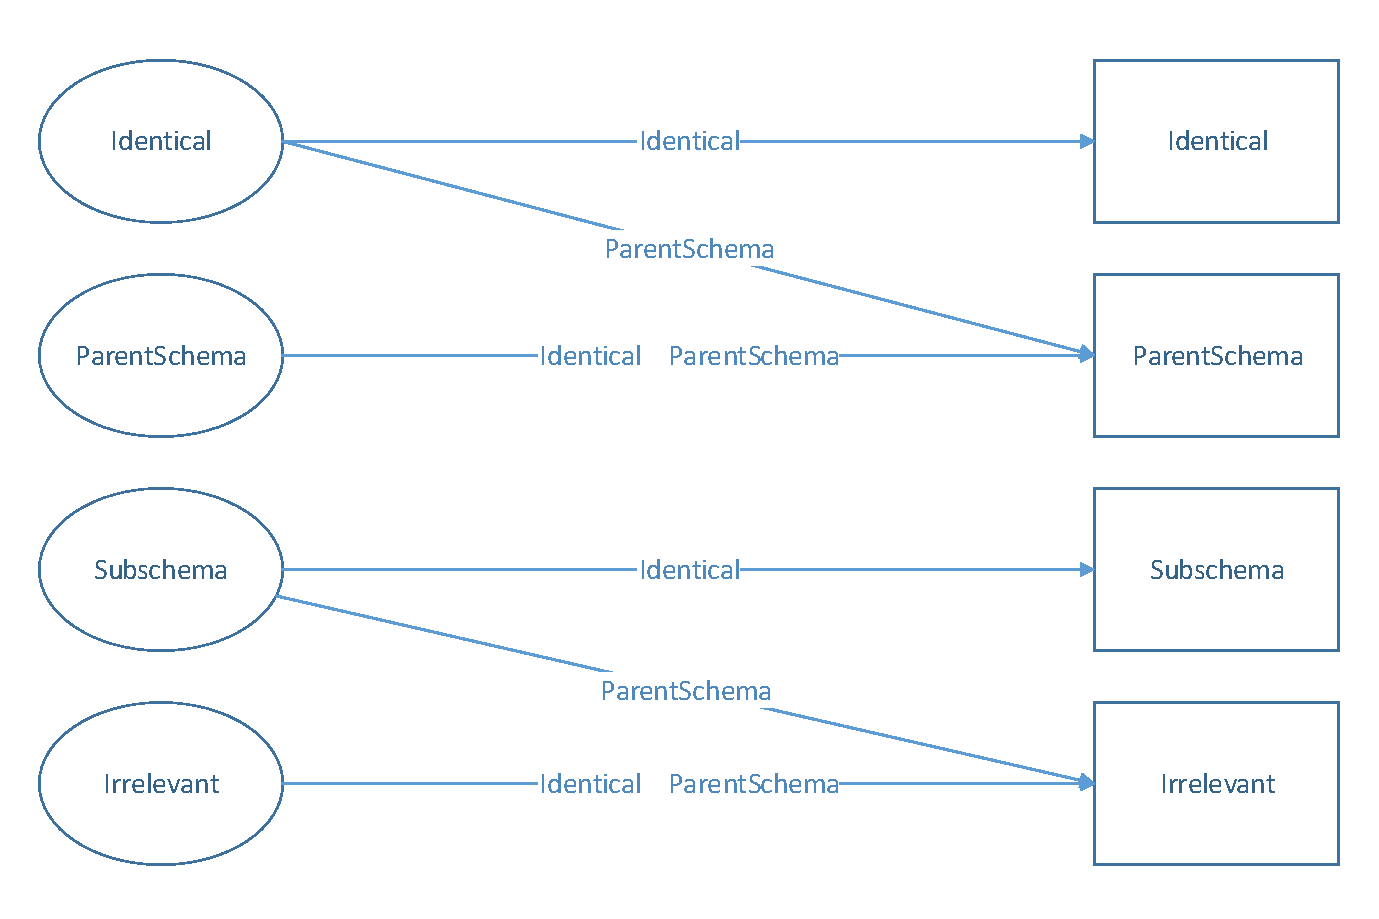
\includegraphics[width=4.31in]{fci-mask-influence.eps}
%\caption{masking effects influence on FCI with distinguishing failures}
%\label{fig:fci_mask_distinguish}
%\end{figure}

\begin{table}[h]
\tbl{Masking effects influence on FCI with distinguishing failures strategy
\label{fci_mask_distinguish}}{
\begin{tabular}{|lll|}
\hline
1  & If  $ c_{m} = c_{origin}$ \  and\   $c_{new} = c_{origin}  $                                & Then, $ \exists c_{m}',s.t.,c_{new} = c_{m}'  $             \\
2  &  If  $ c_{m} = c_{origin}$   and\   $c_{origin} \prec  c_{new} $       & Then,  $\exists c_{m}',s.t., c_{m}' \prec c_{new} $              \\
3  & If $c_{m} \prec c_{origin}$\ and\  $c_{new} = c_{origin}  $                 & Then, $\exists c_{m}',s.t.,c_{m}' \prec c_{new} $               \\
4 & If $c_{m} \prec c_{origin}$\  and\ $c_{origin} \prec c_{new}$                 & Then, $c_{m}',s.t., c_{m}' \prec c_{new}$        \\
5  & If $c_{origin} \prec c_{m}$\ and\ $c_{new} = c_{origin}  $          & Then, $\exists c_{m}',s.t.,c_{new} \prec c_{m}' $               \\
6a  & If $c_{origin} \prec c_{m}$\  and\ $c_{origin} \prec c_{new} $      & Then either $\exists  c_{m}',s.t.,c_{new} = c_{m}'  $              \\
6b &  & Or $\exists  c_{m}',s.t., c_{m}' \prec c_{new} $    \\ %\hline
6c &  & Or $\exists  c_{m}',s.t.,c_{new} \prec c_{m}'  $    \\
6d &  & Or $c_{new}\  irrelevant\ all\ c_{m}' $    \\
7  & If $c_{origin}\ irrelevant\ all\ c_{m}$\ and\ $c_{new} = c_{origin} $                  & Then, $ c_{new}\ irrelevant\ to\ all\ c_{m}'$ \\
8a & If $c_{origin}\ irrelevant\ all\ c_{m}$\ and\ $c_{origin} \prec c_{new}$     & Then either,$\exists c_{m}',s.t.,c_{m}' \prec c_{origin}$         \\
8b &                                                                                      & Or,$c_{new}\ irrelevant\ to\ all\ c_{m}'  $ \\ %\hline
%9a &                         if $c_{new}\ irrelevant\ to\ all\ c_{origin}$ & Then either,$\exists c_{m}',s.t., c_{m}' \prec c_{new} $        \\
%9b &                                                             & Or,$ c_{new}\ irrelevant\ to\ all\ c_{m}'$  \\

9 & It may have $c_{origin}\ irrelevant\ to\ all\ c_{new}$  & \\\hline
\end{tabular}}
\end{table}


Similar to Table \ref{fci_mask_regard}, this table also lists the possible relationships among the schemas that are gotten by strategy \emph{distinguishing failures}, schemas that are gotten by \emph{knowing masking effects} strategy, and the actual MFS. As with the \emph{distinguishing failures} strategy, the minimal schemas identified are actually $\mathcal{C}(A \bigcup B_{1} \bigcup C)$.  Obviously $A \bigcup B_{1} \bigcup C \subset A \bigcup B_{1} \bigcup B_{2} \bigcup C $. So with this strategy, $c_{new} \in \mathcal{C}(A \bigcup B_{1} \bigcup C)$ should be either the parent-schema or identical to $c_{origin} \in \mathcal{C}( A \bigcup B_{1} \bigcup B_{2} \bigcup C)$.  The main difference between the rules in Table \ref{fci_mask_distinguish} and rules in Table \ref{fci_mask_regard} is that most rules with strategy \emph{distinguishing failures} result in that $c_{m}' \prec c_{new}$. This is because with strategy \emph{distinguishing failures}, the test cases that are used for identifying the MFS is less than that of \emph{knowing masking effects}. So more likely it may have $\mathcal{T} (c_{new}) \subset \mathcal{T} (c_{m}') $, and hence $c_{m}' \prec c_{new}$.

We take an example to illustrate these rules of strategy \emph{distinguishing failures}, which is depicted in Table \ref{example-of-fci-influence-distiguish}. Similar to our previous strategy, we omit the samples that have the condition `$c_{origin} = c_{new}$'.

One rule that is needed to be noted is rule 10, which can make some $c_{origin}$ \emph{removed} from the newly minimal schemas, i.e., $\not\exists c_{new}, s.t., c_{new} = c_{origin}\ or\ c_{origin} \prec c_{new}$.  For the Table \ref{example-of-fci-influence-distiguish} example, in the last row for the rule 10, we can find the schema $c_{origin}--$(1,1,0,0,1,-), which is identical to the one in actual MFS, there exists no $c_{new}$ which is identical to or is the parent-schema of this schema. Consequently, in this condition, this strategy may ignore some actual MFS compared with \emph{knowing masking effects}.

In fact, besides this special case that may result in the FCI approach ignoring some actual MFS, there exist some other cases that can also achieve the same effect. For example, when the $c_{new}$ is the only schema that is \emph{related} to $c_{origin}$, (\emph{related} means not irrelevant, and in this case it is either identical to or the parent-schema). And the corresponding parent-schema $c_{origin}$ is the only schema which is related to one actual MFS $c_{m}$. Then, if the $c_{new}$ is irrelevant to all the actual MFS, we will ignore the actual MFS $c_{m}$. This \emph{ignored} event is caused by the $c_{new}$ growing into the irrelevant schemas, which can also appear in the strategy \emph{regarded as one failure}. However, the aforementioned cause of \emph{ignored}--the $c_{origin}$ is \emph{removed} from the newly minimal schemas can only happen in the strategy \emph{distinguishing failures}.
%This appears when $T(c_{origin}) \subset B_{2}$, as such that all the test cases contain $c_{origin}$ will be ignored with the strategy \emph{distinguish failures}. When this transformation happens, no more other relationship between $c_{new}$ and $c_{m}$ increased, but it make the newly minimal schemas \emph{ignore} some actual MFS as we discussed before.

%Similarly, we just give the proof of some transformation that is not so obviously.
%\begin{proposition}
%Original sub-schema, the parent-schema must be irrelevant.
%
%\end{proposition}
%\begin{proof}
%Without loss of generality, we assume $c$ is sub-schema to the actual MFS, say, $c_{n}$. Then $T(c)$ must contain some other test cases in $A$. After using the  \emph{distinguish  failures} strategy, if we have $c \prec c'$, then $T(c')$ must lose some test cases in $B_{2}$.(If not so, there must be no c').
%
%So as it contain other test cases in $A$ and lose some test case in $B_{2}$. It cannot be the parent and identical to the MFS. If it is sub-schema of some MFS, say $c_{m}$. Then we must have $T(c_{m}) \subset T(c_{n})$. As Both $c_{m}$ and $c_{n}$ are MFS, which contradicts.
%\end{proof}
%
%
%\begin{proposition}
%Original identical-schema, the parent-schema must be irrelevant.
%
%\end{proposition}
%\begin{proof}
%Without loss of generality, we assume $c$ is irrelevant to the actual MFS, say, $c_{n}$. Then $T(c)$ must contain some other test cases in $A$. After using the  \emph{distinguish  failures} strategy, if we have $c \prec c'$, then $T(c')$ must lose some test cases in $B_{2}$.(If not so, there must be no c').
%
%So as it contain other test cases in $A$ and lose some test case in $B_{2}$. It cannot be the parent and identical to the MFS. If it is sub-schema of some MFS, say $c_{m}$. Then we must have $T(c_{m}) \subset T(c_{n})$. As Both $c_{m}$ and $c_{n}$ are MFS, which contradicts.
%\end{proof}
%
%Another point need to be noted is that this transformation also mean some ignored ones(As MFS irrelevant to the set).

\begin{table}
\tbl{Example the influence of distinguishing failures for FCI approach\label{example-of-fci-influence-distiguish}}{
\begin{tabular}{llllllllllll}
%\multicolumn{3}{c}{} &\multicolumn{3}{c}{}  & \multicolumn{3}{c}{} & \multicolumn{3}{c}{}\\
\multicolumn{3}{c}{\bfseries $A$} &\multicolumn{3}{c}{\bfseries $B_{1}\bigcup C$}  & \multicolumn{3}{c}{\bfseries $B_{2}$} & \multicolumn{3}{c}{\bfseries $D$}\\ \hline

\multicolumn{3}{c}{(0,0,0,1,1,0)}&\multicolumn{3}{c}{(0,0,0,0,0,0)}&\multicolumn{3}{c}{(0,0,1,1,1,0)}&\multicolumn{3}{c}{(0,1,1,0,0,0)}\\
\multicolumn{3}{c}{(0,0,1,1,0,0)}&\multicolumn{3}{c}{(0,0,0,0,1,0)}&\multicolumn{3}{c}{(1,1,0,1,0,0)}&\multicolumn{3}{c}{(0,1,1,0,1,0)}\\
\multicolumn{3}{c}{(0,0,1,0,1,0)}&\multicolumn{3}{c}{(0,0,0,1,0,0)} & \multicolumn{3}{c}{(1,0,1,1,0,1)}&\multicolumn{3}{c}{(0,1,1,1,0,0)}\\
\multicolumn{3}{c}{(0,0,1,0,0,0)}&\multicolumn{3}{c}{(1,1,1,1,1,0)} & \multicolumn{3}{c}{(0,0,1,1,1,1)}&\multicolumn{3}{c}{(0,1,1,1,1,0)}\\
\multicolumn{3}{c}{(1,1,0,0,0,0)} &\multicolumn{3}{c}{(1,1,0,0,1,0)} & \multicolumn{3}{c}{(1,1,0,0,1,1)}&\multicolumn{3}{c}{(1,1,1,1,1,1)}\\
\multicolumn{3}{c}{(0,0,1,1,0,1)} &\multicolumn{3}{c}{(1,1,0,1,1,0)} & \multicolumn{3}{c}{(0,1,0,0,1,1)} & \multicolumn{3}{c}{(0,1,1,1,1,1)}\\
\multicolumn{3}{c}{} &\multicolumn{3}{c}{(1,1,1,0,0,0)} & \multicolumn{3}{c}{(1,0,1,0,1,1)} & \multicolumn{3}{c}{(1,1,1,1,0,1)}\\
\multicolumn{3}{c}{} &\multicolumn{3}{c}{(1,1,1,1,0,0)} & \multicolumn{3}{c}{} & \multicolumn{3}{c}{(1,0,0,1,1,1)}\\
\multicolumn{3}{c}{} &\multicolumn{3}{c}{(1,1,1,0,1,0)} & \multicolumn{3}{c}{} & \multicolumn{3}{c}{}\\
\multicolumn{3}{c}{} &\multicolumn{3}{c}{(1,0,1,1,1,1)} & \multicolumn{3}{c}{} & \multicolumn{3}{c}{}\\
\multicolumn{3}{c}{} &\multicolumn{3}{c}{(0,0,0,0,1,1)} & \multicolumn{3}{c}{} & \multicolumn{3}{c}{}\\
\multicolumn{3}{c}{} &\multicolumn{3}{c}{(1,0,0,0,1,1)} & \multicolumn{3}{c}{} & \multicolumn{3}{c}{}\\
 \hline
\multicolumn{4}{c}{\bfseries $actual\ MFS$} &\multicolumn{4}{c}{\bfseries $knowing\ masking\ effects$} & \multicolumn{4}{c}{\bfseries $distinguishing failures$} \\
\multicolumn{4}{c}{\bfseries $\mathcal{C}(B_{1} \bigcup B_{2} \bigcup C \bigcup D )$} &\multicolumn{4}{c}{\bfseries $\mathcal{C}(A \bigcup B_{1} \bigcup B_{2} \bigcup C)$} & \multicolumn{4}{c}{\bfseries $\mathcal{C}(A \bigcup B_{1} \bigcup C)$} \\ \hline
\multicolumn{4}{c}{(0,-,1,1,1,-) } &\multicolumn{4}{c}{(1,1,-,-,-,0)} & \multicolumn{4}{c}{(0,0,0,-,-,0)} \\
\multicolumn{4}{c}{(1,1,-,1,-,0) } &\multicolumn{4}{c}{(0,0,-,-,-,0)} & \multicolumn{4}{c}{(0,0,-,-,0,0)}\\
\multicolumn{4}{c}{(-,-,0,0,1,1) } &\multicolumn{4}{c}{(-,0,1,1,-,1)} & \multicolumn{4}{c}{(0,0,-,0,-,0)}\\
\multicolumn{4}{c}{(0,0,0,-,0,0)}  &\multicolumn{4}{c}{(0,0,1,1,-,-)} & \multicolumn{4}{c}{(1,1,1,-,-,0)} \\
\multicolumn{4}{c}{(0,0,0,0,-,0)}  &\multicolumn{4}{c}{(0,0,0,0,1,-)} &  \multicolumn{4}{c}{(1,1,-,-,1,0)} \\
\multicolumn{4}{c}{(1,0,-,-,1,1)}  &\multicolumn{4}{c}{(1,1,0,0,1,-)} & \multicolumn{4}{c}{(1,1,-,0,-,0)}\\
\multicolumn{4}{c}{(1,1,0,0,1,-)}  &\multicolumn{4}{c}{(1,0,1,-,1,1)} & \multicolumn{4}{c}{(0,0,1,1,0,-)}\\
\multicolumn{4}{c}{(-,1,1,-,-,0)}  &\multicolumn{4}{c}{(1,0,-,0,1,1)} & \multicolumn{4}{c}{(1,0,1,1,1,1)}\\
\multicolumn{4}{c}{(-,-,1,1,1,1)}  &\multicolumn{4}{c}{(-,-,0,0,1,1)} & \multicolumn{4}{c}{(-,0,0,0,1,1)}\\
\multicolumn{4}{c}{(1,1,-,-,1,0)}  &\multicolumn{4}{c}{} & \multicolumn{4}{c}{(0,0,0,0,1,-)}\\
\multicolumn{4}{c}{(-,1,1,1,1,-)}  &\multicolumn{4}{c}{} & \multicolumn{4}{c}{}\\
\multicolumn{4}{c}{(1,1,1,1,-,-)}  &\multicolumn{4}{c}{} & \multicolumn{4}{c}{}\\
\multicolumn{4}{c}{(1,-,1,1,-,1)}  &\multicolumn{4}{c}{} & \multicolumn{4}{c}{}\\
\multicolumn{4}{c}{(0,0,0,0,1,-)}  &\multicolumn{4}{c}{} & \multicolumn{4}{c}{}\\

\multicolumn{4}{c}{\bfseries rules} &\multicolumn{2}{c}{\bfseries $c_{m}$}  & \multicolumn{2}{c}{\bfseries $c_{origin}$} & \multicolumn{2}{c}{\bfseries $c_{new}$} & \multicolumn{2}{c}{\bfseries $c_{m}'$}\\ \hline
\multicolumn{4}{c}{2} &\multicolumn{2}{c}{(-,-,0,0,1,1)}  & \multicolumn{2}{c}{(-,-,0,0,1,1)} & \multicolumn{2}{c}{(-,0,0,0,1,1)} & \multicolumn{2}{c}{(-,-,0,0,1,1)}\\
\multicolumn{4}{c}{4} &\multicolumn{2}{c}{(1,0,-,-,1,1)}  & \multicolumn{2}{c}{(1,0,1,-,1,1)} & \multicolumn{2}{c}{((1,0,1,1,1,1))} &\multicolumn{2}{c}{((1,0,-,-,1,1))} \\
\multicolumn{4}{c}{6d} &\multicolumn{2}{c}{(1,1,-,1,-,0) }  & \multicolumn{2}{c}{(1,1,-,-,-,0)} & \multicolumn{2}{c}{(1,1,-,0,-,0)} & \multicolumn{2}{c}{*} \\
\multicolumn{4}{c}{6c} &\multicolumn{2}{c}{(0,0,0,0,-,0)}  & \multicolumn{2}{c}{(0,0,-,-,-,0) } & \multicolumn{2}{c}{(0,0,0,-,-,0)} &  \multicolumn{2}{c}{(0,0,0,0,-,0)}\\
\multicolumn{4}{c}{6b} &\multicolumn{2}{c}{(1,1,-,1,-,0)}  & \multicolumn{2}{c}{(1,1,-,-,-,0) } & \multicolumn{2}{c}{(1,1,1,-,-,0)} &  \multicolumn{2}{c}{(-,1,1,-,-,0)}\\
\multicolumn{4}{c}{6a} &\multicolumn{2}{c}{(1,1,-,-,1,0)}  & \multicolumn{2}{c}{(1,1,-,-,-,0) } & \multicolumn{2}{c}{(1,1,-,-,1,0)} &  \multicolumn{2}{c}{(1,1,-,-,1,0)}\\
\multicolumn{4}{c}{8a} &\multicolumn{2}{c}{*}  & \multicolumn{2}{c}{(-,0,1,1,-,1)} & \multicolumn{2}{c}{(1,0,1,1,1,1)} & \multicolumn{2}{c}{(1,-,1,1,-,1)}\\
\multicolumn{4}{c}{8b} &\multicolumn{2}{c}{*}  & \multicolumn{2}{c}{(0,0,1,1,-,-) } & \multicolumn{2}{c}{(0,0,1,1,0,-)} & \multicolumn{2}{c}{*}\\

\multicolumn{4}{c}{9} &\multicolumn{2}{c}{(1,1,0,0,1,-)}  & \multicolumn{2}{c}{(1,1,0,0,1,-)} & \multicolumn{2}{c}{*} & \multicolumn{2}{c}{*}\\
%\multicolumn{4}{c}{$c_{new_{irrele}} \prec c_{m}'$} &\multicolumn{2}{c}{*}  & \multicolumn{2}{c}{*} & \multicolumn{2}{c}{(-,0,-,0,-,0)} & \multicolumn{2}{c}{(0,0,0,0,-,0)} \\
%\multicolumn{4}{c}{$c_{new_{irrele}}\ irrele$} &\multicolumn{2}{c}{*}  & \multicolumn{2}{c}{*} & \multicolumn{2}{c}{(1,-,1,1,1,-)}& \multicolumn{2}{c}{*}\\

\end{tabular}}
\end{table}
%So what this two mutation than is , we first learn that
%
%So actually, when encountering masking effects, both this two strategies is not good.
%Previous analysis just based on the the observed changed, in fact, the if we changing the analysis, the pridicted and observed will aslo be changed?

%In fact, the masking effects firstly change the $T_{fail_{observed}}$, as masking effects, FCI either will identify $T_{fail_{observed}}$ less or more than it expected to be, as a consequence, regardless of $T_{fail_{predicted}}$ can be, masking effects makes FCI approaches never reach a perfect result, i.e., accurately and completely find each MFS.
%
%Secondly, as $T_{fail_{observed}}$ changed, $T_{fail_{predicted}}$ consequently changed. As a result, if $T_{fail_{predicted}}$ it can accurate predict without masking effects, then masking effects obviously makes the FCI approaches worse. However, if it originally cannot predicted inaccurately, then this changing will have a possibility make the $T_{fail_{observed}}$ changing better, and of course, it also can have a possibility make the $ T_{fail_{predicted}}$ changing worse.

\subsection{Summary of the masking effects on the FCI approach}
From the analysis of the formal model, we can learn that masking effects do influence the FCI approaches, and even worse, both the \emph{regarded as one failure} and \emph{distinguishing failures} strategies are harmful. Specifically when compared with the \emph{knowing masking effects} condition, the strategy \emph{regarded as one failure} has a larger possibility of getting more sub-schemas of the actual MFS and getting more schemas which are irrelevant to the MFS, while strategy \emph{distinguishing failures}  may get more parent schemas of the MFS and can also get more irrelevant MFS. Further, both strategies can ignore the actual MFS and the \emph{distinguishing failures} strategy is more likely to ignore the MFS than the \emph{regarded as one failure} strategy.

%Note that our discussion is based on a SUT using deterministic software, i.e., the random failing information of a test case will be ignored. The non-deterministic problem will result in a more complex test scenario, which will not be discussed in this paper.

\section{Test case replacing strategy}
%Previous section formally studied the case that under the masking effects, neither regarding as one failure approach nor distinguishing failures approach is not accurate .
The main reason why the FCI approach fails to properly work is that we cannot determine the areas $B_{2}$ and $B_{3}$, i.e., if the test case trigger other failures which are different from the current one, we cannot figure out whether this test case will trigger the current expected failure as the masking effects may prevent that. So to limit the impact of this effect on the FCI approach, we should make efforts to reduce the number of test cases that trigger other different failures, so that we can reduce the possibility that expected failure may be masked by other failures.
% strategies cannot accurately identify the MFS is that we cannot figure out the $T(mask_{F_{m}})$.  As $T(mask_{F_{m}}) \subset \bigcup_{i = 1 \& i \neq m }^{L}T_{F_{i}}$, in order to weaken the influence of $T(mask_{F_{m}})$, we need to reduce the number of test cases that trigger other failures as much as possible.

In the exhaustive testing, as all the test cases will be used to identify the MFS, there is no room left to improve the performance unless we fix other failures and re-execute all the test cases. However, when you just need to select part of all the test cases to identify the MFS (which is how the traditional FCI approach works), we can adjust the test cases we need to use by selecting the proper ones. By doing this, we can limit the size of $\mathcal{T}(mask_{F_{m}})$ to be as small as possible.

\subsection{Replacing test cases that trigger unexpected failures}

The basic idea is to pick the test cases that trigger other failures and generate new test cases to replace them. These regenerated test cases should either pass in the execution or trigger $F_{m}$. The replacement must satisfy the condition that the newly generated ones will not negatively influence the original identifying process.

Commonly, when we replace the test case that triggers an unexpected failure with a new test case, we should keep some part in the original test case. We call this part the \emph{fixed part}, and mutate the other part with different values from the original one. For example, if a test case (1,1,1,1) triggered an unexpected failure, and the fixed part is (-,-,1,1). Then, we can replace it with a test case (0,0,1,1) which may either pass or trigger the expected failure.

The \emph{fixed part} can vary for different FCI approaches, e.g, for the OFOT \cite{nie2011minimal} algorithm, the parameter values are the fixed part except for the one that needs to be validated, while for the FIC\_BS \cite{zhang2011characterizing} approach, we will fix the parameter values that should not be mutated for the test case in the next iteration of the FIC\_BS process.

We note that this replacement may need to be executed multiple times for one fixed part as we could not always find a test case that coincidentally satisfied our requirement. One replacement method is randomly choosing test cases until the satisfied test case is found. While this method may be simple and straightforward, however, it also may require trying too many times to get the satisfied one. So to handle this problem and reduce the cost, we proposed a replacement approach by computing the \emph{strength} of the test case with the other failures, and then we selected the test case from a group of candidate test cases that has the least \emph{strength} related to the other failures.

% which during the originally test, record the test cases that trigger other test cases and next replacement process will consult this set to avoid some test cases with a high probability to trigger other failures.

To explain the \emph{strength} notion, we need first to introduce the \emph{strength} that a parameter values is related to a particular failure. We use $all(o)$ to represent the number of executed test cases that contain this parameter value, and $m(o)$ to indicate the number of test cases that trigger the failure $F_{m}$ and contain this parameter value. Then, the \emph{strength} that a parameter value is related to a particular failure, i.e., $S(o, F_{m})$, is $\frac{m(o)}{all(o) + 1}$. This heuristic formula is based on the idea that if a parameter value frequently appears in the test cases that trigger the particular failure, then it is more likely to be the inducing factor that triggers this type of failure. We add 1 in the denominator for two facts:  (1) avoid division by zero when the parameter value has never appeared before, (2) reduce the bias when a parameter value rarely appears in the test set but coincidentally appears in a failing test case with a particular failure.

With this \emph{strength} definition for a parameter value, we then define that the \emph{strength} of a test case $f$ is related to a particular failure $F_{m}$ as:

\begin{displaymath} S(f,F_{m})  = \frac{1}{k}\sum_{o \in f} S(o, F_{m}) \end{displaymath}

In this formula, $k$ is the number of parameters in the test case $f$, $o$ is the specific parameter value in $f$. Then this formula defines the \emph{strength} that a test case is related to a failure as the average \emph{strength} of the relevance between each parameter value in the test case and this failure. For a test case that is selected to be tested, we want that the ability of that test case to trigger another failure to be as small as possible. In practice, the relevance \emph{strength} varies between one test case with different failures. As a result, we cannot always find a test case that, for any failure, the \emph{strength} that this test case is related to that failure is the least.  With this in mind, we have to settle for a test case, such that the maximal possible failure (except for the one that is currently analysed) it can trigger should be the least likely to be triggered when compared with that of other test cases. In another word, we need to find a test case, so that the maximal \emph{strength} that it is related to a failure is minimal. Formally, we should choose a test case $f$, s.t.,

\begin{displaymath} \min_{f \in R} \max_{m \leq L \& m \neq n}  S(f, F_{m}) \tag{EQ1} \end{displaymath}

In this formula, $L$ is the number of all the failures, and $n$ is the current analysed failure. $R$ is the set of all the possible test cases that contain the $fixed$ part except those that have been tested. To choose the test case from the set $R$ is because the FCI approach needs to keep the $fixed$ part when generating additional test cases and surely we need to select a test case that has not been tested yet. Obviously $|R| = \prod_{i \not\in fixed}(v_{i})\ - |\{t\ |\ t\ contains\ the\ fixed\ part\ \&\ t\ is\ tested\}|$.

We can further resolve this problem. Consider the test case we get -- $f$ satisfied the EQ1. Without loss of generality, we assume that the failure $F_{k}, k \neq n $ is the failure with which the test case $f$ has the maximal related \emph{strength} compared to the other failures. Then, a natural property for $f$ is that any other test case $f'$ which satisfies that failure $F_{k}$ is the maximal related failure for this test case
and must have $ S(f, F_{k}) <= S(f', F_{k})$. Formally, to get such a test case is to solve the following formula:

\begin{alignat}{2}
\min\quad &  S(f, F_{k}) &{}& \tag{EQ2} \label{eqn - lp}\\
\mbox{s.t.}\quad
&f \in R &\quad& {}\nonumber\\
&S(f, F_{k}) > S(f, F_{i}), &{}& 1 \leq i \leq L\ \&\ i\neq k, n \nonumber
\end{alignat}

With this formula, to solve EQ1, we just need to find the particular failure $F_{k}$, such that the related \emph{strength} between the test case $f$ that satisfies EQ2 and this failure is the smallest than that of the other failures. Formally, we need to find:
\begin{alignat}{2}
\min\quad &  S(f, F_{k}) &{}& \tag{EQ3} \label{eqn - 2p}\\
\mbox{s.t.}\quad
& 1 \leq k \leq L \ \& \ k \neq n &\quad& {}\nonumber\\
& f , F_{k}\ satisfies\ EQ2 &{}& {} \nonumber
\end{alignat}

According to EQ3, the problem to get such a test case lies in solving EQ2 because if EQ2 is solved we just need to rank the one that has the minimal value from the solutions to EQ2. As to EQ2, it can be formulated as an 0-1 integer linear programming (ILP) problem. Assume the SUT we test has $K$ parameters in which the $i$th parameter has $V_{i}$ values it can take from. And the SUT has $L$ failures. We then define the variable $x_{ij}$ as:
\begin{displaymath}
x_{ij} = \begin{cases}1 & the\ \emph{i}th\ parameter\ of\ the\ test\ case\ take\ the\ \emph{j}th\ value\ for\ that\ parameter\\0 & otherwise\end{cases}
\end{displaymath}
We then take $o_{m_{ij}}$ to be the related \emph{strength} between the \emph{j}th value of the \emph{i}th parameter of the SUT and the failure $F_{m}$. And we use a set $R$ of parameter values to define the fixed part in the test case we should not change, i.e., $R = \{(i, j) |i\ is\ the\ fixed\ parameter\ in\ the\ test\ case, j\ is\ the\ corresponding\ value\}$. As we can generate redundant test cases, so we keep a set of test cases $T_{executed}$ to guide to generate different test cases. Then EQ2 can be detailed as the in following ILP formula:

\begin{alignat}{2}
\min\quad & \frac{1}{|K|}\sum_{i = 0}^{K}\sum_{j = 0}^{V_{i}}  o_{m_{ij}} \times x_{ij} &{}& \tag{EQ4} \label{eqn - 3p}\\
\mbox{s.t.}\quad
& 0 \leq x_{ij} \leq 1 &\quad& { i = 0 .. K - 1, j = 0,.. V_{i} - 1 }\\
&  x_{ij} \in  \mathbb{Z}&\quad& { i = 0 .. K - 1, j = 0,.. V_{i} - 1 }\\
& \sum_{j = 0}^{V_{j}} x_{ij} = 1&\quad& { i = 0 ... K - 1}\\
&  x_{ij} = 1 &\quad& { (i,j) \in R }\\
& \sum_{i = 0}^{K}\sum_{j = 0}^{V_{i}} (o_{m_{ij}} - o_{m'_{ij}})\times  x_{ij} \geq 0 &\quad& {1 \leq m' \neq m \leq L}\\
& \sum_{(i,j) \in t}  x_{ij} < K &\quad& {t \in T_{existed}}
\end{alignat}

In this formula, constraints (1) and (2) indicate that the variable $x_{ij}$ is a 0-1 integer. Constraint (3) indicates that a parameter in one test case can only take one value. Constraint (4) indicates the test case should not change values of the fixed part. Constraint (5) indicates that the related strength between the test case and Failure $F_{m}$ is higher than that of the other failures. Constraint (6) indicates the test cases generated should not be the same as the test cases in $T_{existed}$

As we have formulated the problem into a 0-1 integer programming problem, we just need to utilize an ILP solver to solve this formula. In this paper, we use the solver introduced in \cite{Berkelaar2004}, which is a mixed Integer Linear Programming (MILP) solver that can handle satisfaction and optimization problems.
%this actually an integer programming problem, as the test case $f$ is the vector of component $o$, which is concrete variable. However, it dose not belongs to the integer linear programming (ILP) problem, because the objective function  $S(f, F_{k})$, i.e., $\frac{1}{|f|}\sum_{o \in f} S(o, F_{m})$, is not linear to the component $o$.
%s.t.
%
%S(f, F_{k}) > S(f, F_{1})
%S(f, F_{k}) > S(f, F_{2})
%...
%S(f, F_{k}) > S(f, F_{n-1})
%S(f, F_{k}) > S(f, F_{n+1})
%...
%S(f, F_{k}) > S(f, F_{L})
% So to make it as less as possible is actually make the test case $f$ less related to other failures.

The complete process of replacing a test case with a new one while keeping some fixed part is depicted in Algorithm 1:

\begin{algorithm}[t]
%\SetAlgoNoLine
\KwIn{ failure type $F_{m}$,fixed part $s_{fixed}$, set of values that each option can take $Param$, the related strength matrix $o_{1} ... o_{L}$}
\KwOut{ $t_{new}$ the regenerate test case,The frequency number }
%$index$ = 0; $FreNum_{\alpha}$ = -1\;
\While{\textbf{not} MeetEndCriteria()}{
       $optimal \leftarrow MAX$ ;
       $t_{new} \leftarrow null$ \;
       \ForAll {$F_{k} \in {F_{1},...F_{m}, F_{m+1} ... F_{L}}$}{
                $solver \leftarrow setup(s_{fixed}, Param, F_{m}, o_{1} ... o_{L})$\;
                $(optimal', t_{new}') \leftarrow solver.getOptimalTest()$ \;
                \If {$optimal' < optimal$}{
                       $t_{new} \leftarrow t_{new}'$\;
                    }
          }
       $result \leftarrow execute(t_{new})$\;
       $updatetRelatedStrengthMatrix(t_{new})$ \;
        \eIf {$result == PASS\ or\ result ==  F_{m}$}{
         \Return $t_{new}$\;
           }{
         continue\;
         }
       }
       \Return \emph{null}

\caption{Replacing test cases triggering unexpected failures}
\label{alg:one}
\end{algorithm}

The inputs for this algorithm consist of the failure type we focus on -- $F_{m}$, the fixed part of which we want to keep from the original test case -- $s_{fixed}$ , the set of values that each parameter can take from respectively -- $Param$ and the set of matrix $o_{1},...o_{L}$, for any element in which, say $o_{m}$, is recorded the related strength between each specific parameter with each value and the failure $F_{m}$, i.e., $o_{m} = \{o_{m_{ij}} | 0 \leq i \leq K - 1, 0 \leq j \leq V_{i}\}$. The output of this algorithm is a test case $t_{new}$ which either triggers the expected $F_{m}$ or passes.

This algorithm is an outer loop (lines 1 - 19) containing two parts:

The first part (lines 2 - 9) generates a new test case which is supposed to be least likely to trigger failures different from $F_{m}$. The basic idea for this part is to search each failure different from $F_{m}$ (line 3) and find the best test case that has the least related strength with other failures. In detail, for each failure we set up an ILP solver (line 4) and use it to get an optimal test case for that failure according to EQ4 (line 5). We compare the optimal value for each failure, and choose the one has less strength related to other failures (lines 6 - 9).
%Different from the original algorithm, we generate a set of candidate test cases (line 3 - 11) instead of only one, and then choose the one that has the least possibility that is related to other failures(line 12) according to our previous formula. Our candidate set of test cases is initialed as size \emph{N}, the specific number it is assigned is a tradeoff between how quickly this algorithm ended in getting a candidate test case and how many times you'd like to try to find a really satisfied test case. It is noted that when \emph{N} = 1, it grows into our previous algorithm. Each test cases in the candidate set is generated by random(line 4 - 11), they must be different from existed test cases(we don't show in this pseudo code) and each one of them should keep the fixed part (line 9), and just mutate the factors which are not in that part(line 2). The mutation for each factor works by selecting one legal value which is different from the original one(line 5 - 8).
%The generated newly test case must be different from each iteration(we implemented it by hashing method).

The second part is to check whether the newly generated test case is as expected (lines 10 - 16). We first execute the SUT under the newly generated test case (line 10) and update the related strength matrix ($o_{1} ... o_{L}$) for each parameter value that is involved in this newly generated test case (line 11). We then check the execute result. If either the test case passes or triggers the same failure -- $F_{m}$, we will get an satisfied test case (line 12), and we will directly return this test case (line 13). Otherwise, we will repeat the process, i.e., generate a new test case and check again (lines 14 - 15).

Note that this algorithm has another exit, besides we find an expected test case (line 12), which is when the function \emph{MeetEndCriteria()} returns \emph{true} (line 1). We didn't explicitly show what the function \emph{MeetEndCriteria()} is like, because this is dependent on the computing resource and how accurate you want the identifying result to be. In detail, if you want to get a high quality result and you have enough computing resource, you can try many times to get the expected test case; otherwise, a relatively small number of attempts is recommended.

In this paper, we just set 3 as the greatest number of repeats for this function. When it ends with \emph{MeetEndCriteria()} is true, we will return null(line 18), which means we cannot find an expected test case.

\subsection{A case study using the replacement strategy}
%Next we will take the FCI approach--OFOT algorithm as the subject to see how our approach works on them.

Suppose we have to test a system with eight parameters, each of which has three options. And when we execute the test case $T_{0}$ -- (0, 0, 0, 0, 0, 0, 0, 0), a failure--$e1$ is triggered. Next, we will use the FCI approach -- FIC\_BS \cite{zhang2011characterizing} with replacement strategy to identify the MFS for the $e1$. Furthermore, there are two more potential failures, $e2$ and $e3$, that may be triggered during the testing; and they will mask the desired failure $e1$. The process is shown in Figure \ref{fig:fci_case_study}. In this figure, there are two main columns. The left main column indicates the executed test cases during testing as well as the executed results, and each executed test case corresponds to a specific label, $T_{1}$ -- $T_{8}$, at the left. The right main column lists the related strength matrix when a test case triggers $e2$ or $e3$. In detail, the matrix records the related strength between each parameter (columns $P1$ -- $P8$) for each value it can take (column v) with the unexpected failure (column F). The executed test case, which is in bold, indicates the one that triggers the other failure and should be replaced in the next iteration.
%the test case which are labeled with a deleted line represent the original test case generated by OFOT, and it will be replaced by the regenerated test case which are labeled with a wave line under it.

The completed MFS identifying process listed in Figure \ref{fig:fci_case_study} works as follows: firstly the original FCI approach determines which $fixed$ part that is needed to be test in each iteration. Then the extra test case will be generated to fill in the remaining part. After executing the extra test case, if the result of the execution is normal, i.e., didn't trigger unexpected failure($e_{2}, e_{3}$), then the original FCI process will continue until the MFS is identified. Otherwise,  the replacement strategy will come to effect if one unexpected failure is triggered. The replacement process will mutate the parameter values that is not in the $fixed$ part according to Algorithm 1. After the replacement process, the control for the MFS identifying process will be passed into the original FCI approach.  Next we will specifically explain how the replacement specifically works with an example in this figure.

From Figure \ref{fig:fci_case_study}, for the test case that triggered $e2$ -- (2, 1, 1, 1, 0, 0, 0, 0) (in this case, the fixed part of the test case is (-, -, -, -, 0, 0, 0, 0), in which the last four parameter values are the same as the original test case $T_{0}$), we generate the related matrix at left. Each element in this matrix is computed as the $\frac{m(o)}{all(o) + 1}$; for example, for the $P7$ parameter with value $0$, we can find two test cases that contain this element, i.e., $T_{0}$ and $T_{1}$, so the all(o) is 2. And only one test case triggers the failure $e2$, which means m(o) = 1. So the final related strength between this parameter value with $e2$ is $\frac{1}{2 + 1} = 0.33$. All the related strength with $e3$ is labeled with a short slash as there is no test case triggering this failure in this iteration.  After this matrix has been determined, we can obtain a optimal test case with the ILP solver, which is $T_{1}'$--(1, 2, 2, 2, 0, 0, 0, 0), with its related strength 0.167, which is smaller than that of the others.

This replacement process trigged each time a new test case that triggered another failure until we finally get the MFS. Sometimes we could not find a satisfied replacing test case in just one trial like $T_{1}$ to $T_{1}'$.  When this happened, we needed to repeat searching the proper test case we desired. For example, for $T_{4}$ which triggered $e3$, we tried three times-- $T_{4}', T_{4}'', T_{4}'''$ to finally get a satisfied one $T_{4}'''$ which passes the testing. Note that the matrix continues to change with the test case generated and executed so that we can adaptively find an optimal one in the current process.
% as in this iteration we did not find the test case triggered .
%
%randomly generate three test cases as the candidate test cases, which are (2 1 0 0 0 0 0 0), (2 2 0 0 0 0 0 0), (1 2 0 0 0 0 0 0) respectively.  For one candidate test case in the set--(2 1 0 0 0 0 0 0), the \emph{strength} it is related to the $Err 2$ can be computed as
%
%$$\frac{1}{8} (\frac{0}{1 + 1} + \frac{1}{1 + 1} + \frac{1}{2 + 1}  + \frac{1}{2 + 1} + \frac{1}{2 + 1} + \frac{1}{3 + 1} + \frac{1}{3 + 1}  + \frac{1}{3 + 1} ) = 0.27083$$
%
%In this formula, each sub item in the right parentheses shows the \emph{strength} for each factor that is related to \emph{Err 2}. For example, for the first factor which has value 2, we can only find one test case $T_{1}$ -- (2 2 1 2 0 0 0 0) contain this factor. This test case passed during testing and no other test case contain this factor. So the M(o) and ALl(o) for this factor is 0 and 1 respectively, and the \emph{strength} it is related to the $Err 2$ is is $\frac{0}{1 + 1}$. For the second factor of candidate test case (2 1 0 0 0 0 0 0), we can only find the test case (1 1 0 0 0 0 0 0 ) contain it and trigger the failure -- $Err 2$. So M(o) and ALl(o) for this factor are both 1, and the corresponding \emph{strength} is $\frac{1}{1 + 1}$. The \emph{strength} of remaining factors in this test case is computed in the same way and finally the average \emph{strength} of all these factors is regard as the \emph{strength} of the candidate test case (2 1 0 0 0 0 0 0) that is related to the failure $Err 2$. We also follow the same way to compute the \emph{strength} that these test cases that is related to $Err 3$, as this type failure is never triggered currently, so these \emph{strength} are all 0.
%
%After computed the \emph{strength} for all these candidate test cases, we then choose the one that is least likely to be related to other failures. In this case, we choose the candidate test case (2 2 0 0 0 0 0 0) , its maximal \emph{strength} related to the other failure is against Err 2, which is  0.2083. It is smaller that other two candidate test cases, which both 0.27083. So we choose it as the replaced the test case in the next iteration, i.e., $T_{2}'$.


%
%There is a point need to be noted here, i.e., this approach is actually an augmented random approach, to be exactly choose the one that has the smallest \emph{strength}, we in theory need to rank the $(\prod_{i \in \neg fixed}|v_{i} - 1| - 1)$ (every combination of the value options except the ones in the fixed part) possible candidate test cases. For example, when we find (0 0 1 2 1 2 2 1 ) triggered other failure, we need to select one candidate test case from the set \{(0 0 1 1 1 1 1 1),(0 0 1 1 1 1 1 2),(0 0 1 1 1 1 2 1),(0 0 1 1 1 1 2 2)...(0 0 2 2 2 2 2 2)\}, of which the size is $2^{6} - 1$ (the 1 that is subtracted is the originally test case (0 0 1 2 1 2 2 1 ) triggered other failure). We should note that in the algorithm when we replace the factor value, we do not assign it with the value that appears in the original failing test case, e.g., for  (0 0 1 2 1 2 2 1 ), we will not replace them with test case such as (0 0 0 2 1 0 0 1), this is because we do not want the fixed part we try to test may be interfered with other factors in the original failing test case. So the possible number of test cases we can generate is $(\prod_{i \in \neg fixed}|v_{i} - 1| - 1)$ instead of $(\prod_{i \in \neg fixed}|v_{i}| - 1)$.
%
%It could cause an exponential explosion in the searching space when k is large and fixed part is small. So in this paper we just give this augmented random approach just choose the one "best" test case in a prior given number of randomly generated candidate test cases set. Nevertheless, we believe there may exists other better approaches, e.g., the heuristic approach or greedy approach, may do better at searching a test case with less \emph{strength} related to other failures, which however, will not be discussed in this paper.

%we can find the algorithm mutates one factor to take the different value from the original test case one time. Originally if the test case encounter the result different from the expected error, OFOT will derive the fact that the MFS was broken, in another word, if we change one factor and it does not trigger the expect error, we will label it as one failure-inducing factor, after we changed all the elements, we will get the MFS. For this case, if we take the \emph{regarded as one failure} strategy, then the MFS we got is (- - - 0) because the last case passing test case while the remaining test cases triggered either $Err 1$ or $Err 2$(regarded as one failure).  Additionally when we take the \emph{distinguish failures} strategy, the MFS obtained is (- 0 0 0) as when we changed the second factor, third factor and the fourth factor, it didn't trigger the $Err 1$ ( for second factor, it triggered $Err 2$ and for the third and fourth, it passed).

% So if we do not regenerate the test configuration (0 2 0 0), we will get the MFS -- ( - 0 0 0) for the err 1(which are also labeled with a delete line).

%However, if we replace the test case $t_{2}$--(0 1 0 0) with $t_{2}'$--(0 2 0 0) which triggered err 1 (in this case, the fixed part of the test case is (0, - - -)), and replace the test case $t_{3}$--(0 0 1 0) with $t_{3}'$--(0 0 2 0) which passed, we will find that only when we change the third and fourth factor will we broke the MFS for err 1, therefore,  the failure-inducing combination for err 1 should be (- - 0 0).


%\begin{table}[h]
%\tbl{OFOT with our strategy\label{ofot-aug}}{
%\begin{tabular}{lllllll}
%\multicolumn{5}{c}{\bfseries original test case} & \multicolumn{2}{c}{\bfseries failure info} \\
% $t$ & \multicolumn{4}{l}{0 \ \ \ \ 0 \ \ \ \  0 \ \ \ \  0 } & \multicolumn{2}{c}{Err 1 }\\
% \hline
%$t_{1}$ &\multicolumn{4}{l}{1  \ \ \ \  0 \ \ \ \  0  \ \ \ \  0 }&\multicolumn{2}{c}{ Err 1} \\
%$t_{2}$ &\multicolumn{4}{l}{\sout{0  \ \ \ \  1 \ \ \ \  0  \ \ \ \  0 }} &\multicolumn{2}{c}{ \sout{Err 2}} \\
%         &\multicolumn{4}{l}{0  \ \ \ \  2 \ \ \ \  0  \ \ \ \  0 }& Err 2 :  & Err 3 : \\
%         &\multicolumn{4}{l}{0  \ \ \ \  4 \ \ \ \  0  \ \ \ \  0 }& Err 2 :  & Err 3 : \\
%         &\multicolumn{4}{l}{0  \ \ \ \  5 \ \ \ \  0  \ \ \ \  0 }&Err 2 :   & Err 3 :  \\
%$t_{2}'$ &\multicolumn{4}{l}{\uwave{0  \ \ \ \  2 \ \ \ \  0  \ \ \ \  0}} & \multicolumn{2}{c}{\uwave{Err 1} }\\
%$t_{3}$ &\multicolumn{4}{l}{\sout{0  \ \ \ \  0 \ \ \ \  1  \ \ \ \  0 }} & \multicolumn{2}{c}{\sout{Err 3} }\\
%         &\multicolumn{4}{l}{0  \ \ \ \  0 \ \ \ \  3  \ \ \ \  0 }& Err 2 :  & Err 3 : \\
%         &\multicolumn{4}{l}{0  \ \ \ \  0 \ \ \ \  5  \ \ \ \  0 }& Err 2 :  & Err 3 : \\
%         &\multicolumn{4}{l}{0  \ \ \ \  0 \ \ \ \  7  \ \ \ \  0 }&Err 2 :   & Err 3 :  \\
%$t_{3}'$ &\multicolumn{4}{l}{\sout{0  \ \ \ \  0 \ \ \ \  3  \ \ \ \  0}} & \multicolumn{2}{c}{\sout{Err 3}} \\
%         &\multicolumn{4}{l}{0  \ \ \ \  0 \ \ \ \  2  \ \ \ \  0 }& Err 2 :  & Err 3 : \\
%         &\multicolumn{4}{l}{0  \ \ \ \  0 \ \ \ \  4  \ \ \ \  0 }& Err 2 :  & Err 3 : \\
%         &\multicolumn{4}{l}{0  \ \ \ \  0 \ \ \ \  7  \ \ \ \  0 }&Err 2 :   & Err 3 :  \\
%$t_{3}''$ &\multicolumn{4}{l}{\uwave{0  \ \ \ \  0 \ \ \ \  2  \ \ \ \  0}} & \multicolumn{2}{c}{\uwave{Pass}} \\
%$t_{4}$ &\multicolumn{4}{l}{0  \ \ \ \  0 \ \ \ \  0  \ \ \ \  1} & \multicolumn{2}{c}{Pass} \\
%\hline
%\multicolumn{3}{l}{\bfseries regard as one failure} &  \multicolumn{4}{l}{\bfseries replacing strategy} \\
%\multicolumn{3}{l}{ ( -  \ \ \  - \ \ \  -  \ \ \ 0) } &\multicolumn{4}{l}{ ( -  \ \ \  - \ \ \  0  \ \ \ 0) } \\
%\multicolumn{3}{l}{\bfseries distinguish failures} &\multicolumn{4}{l}{} \\
%\multicolumn{3}{l}{(  -  \ \ \  0 \ \ \  0  \ \ \ 0 )} &\multicolumn{4}{l}{} \\
%\end{tabular}}
%\end{table}

\begin{figure}
\centering
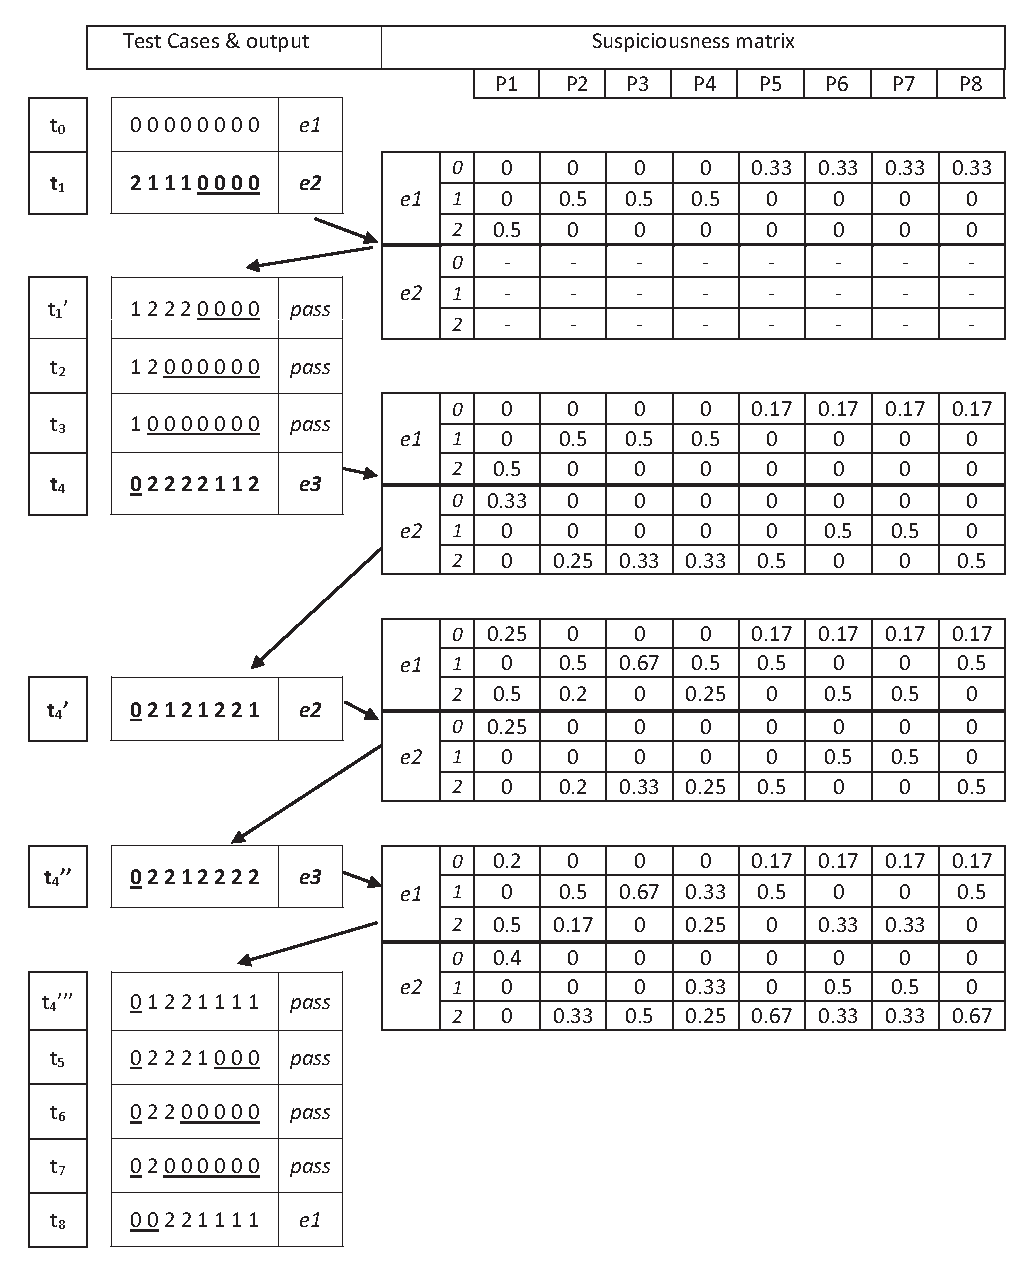
\includegraphics[width=4.31in]{table.eps}
\caption{A case study using our approach}
\label{fig:fci_case_study}
\end{figure}


\subsection{Complexity analysis}
This complexity relies on two facts: the number of test cases that triggered other failures which need to be replaced, and the number of test cases that need to be tried to generate a non-masking-effects test case. The complexity is the product of these two facts.

The first fact is dependent on the extra test cases that are needed to identify the MFS, and this number varies in different FCI approaches. Table \ref{extra-testcases-complexisty} lists the number of test cases that each algorithm needed to get the MFS. In this table, \emph{d} indicates the number of MFS in the SUT. \emph{k} means the number of the parameters of the SUT. \emph{t} is the degree of MFS in the SUT. \emph{c} is an upper bond, and satisfies $d \leq \frac{c}{2} loglog k$. \emph{v} is the number of values one parameter can take.

\begin{table}
\centering
\tbl{The number of test cases each FCI approach needed to identify MFS\label{extra-testcases-complexisty}}{
  \begin{tabular}{c | c}
\bfseries Method & \bfseries number of test cases to identify MFS\\ \hline
Charles ELA & depends on the  covering array \\
Martinez with safe value \cite{martinez2008algorithms,martinez2009locating} & $O(\hat{d}log k + \hat{d}^{2})$ \\
Martinez without safe values \cite{martinez2008algorithms,martinez2009locating} & $O(d^{2} + dlog k + log^{c} k)$  \\
Martinez' ELA \cite{martinez2008algorithms,martinez2009locating} &  $O(ds^{v}log k)$\\
Shi SOFOT \cite{shi2005software}& $O(k)$ \\
Nie OFOT \cite{nie2011minimal} & $O(k \times d)$\\
Ylimaz classification tree & depends on the  covering array\\
FIC \cite{zhang2011characterizing} &  $O(k)$ \\
FIC\_BS \cite{zhang2011characterizing}& $O(t(log k + 1) + 1)$\\
Ghandehari's suspicious based  \cite{ghandehari2012identifying}& depends on the number and size of MFS\\
TRT \cite{niu2013identifying}&  $O(d\times t \times log k + t^{d})$\\
  \end{tabular}
  }
  \end{table}

It must be noted that each algorithm may be limited to some restrictions to identify the result, details of which are shown in \cite{zhang2011characterizing}.

To get the magnitude of the second fact, we need to figure out the possibility of a test case that could trigger other failure. The first thing we need to consider is the \emph{fixed} part, as the additional generated test case should somehow contain this part. As we have mentioned before, we can generate $(v-1)^{k - p} $  (\emph{p} is the number of parameter values in the \emph{fixed} part) possible test cases that contain the \emph{fixed} part. Apart from the one that needs to be replaced, there remain $(v-1)^{k - p}- 1$ candidate test cases, which indicates the complexity is $O((v-1)^{k - p} - 1)$. However, to avoid the exponential computational complexity, in this algorithm we use the method $MeetEndCriteria()$ (line 1) function to end the algorithm when the trying times is over a prior given constant, say $N$, so the final complexity for the second part is $O( min (N, (v-1)^{k - p} - 1))$.
%
%While for adaptive approach, as the $\emph{fixed}$ part is derived from the existed failing test case, which in fact make the test cases to be selected one more less (the existed one), so the complexity is  $O(v^{k - p} - 2)$.

We note that exponent $k - p$ has an significant affect on the complexity of the second fact. The greater $p$ is, the less test cases that can be generated. For a different approach, $p$ is different. For example, for the OFOT approach, $p$ is a fixed number, which is $k - 1$.  And for the FIC\_BS approach, the $p$ varies in the test cases it generates, ranging from $k-1$ to $1$. While for the non-adaptive approaches, as the $fixed $ part is commonly the schemas that are needed to be covered, so the $p$ for these approaches is at least equal to $t$. We have listed all of them in Table \ref{fixed-part-complexisty}. It is noted that the approach -- $Martinez\ without\ safe values$ has no such complexity, because this approach works when $v = 2$, and this results in not having other test cases to be replaced if we test a fixed part when triggering other failures.

\begin{table}
\centering
\tbl{The complexity of the second part\label{fixed-part-complexisty}}{
  \begin{tabular}{c | c}
\bfseries Method & \bfseries fixed part\\ \hline
Charles ELA &   $O( min (N, (v - 1)^{k - t} - 1))$\\
Martinez with safe value \cite{martinez2008algorithms,martinez2009locating} &$O( min (N, (v-1) - 1)) \sim O( min (N, (v-1)^{k - 1} - 1))$\\
Martinez without safe values \cite{martinez2008algorithms,martinez2009locating} &$ - $  \\
Martinez' ELA \cite{martinez2008algorithms,martinez2009locating} & $O( min (N, (v - 1)^{k - t} - 1))$\\
Shi SOFOT \cite{shi2005software}& $O( min (N, (v-1) - 1))) $\\
Nie OFOT \cite{nie2011minimal} & $O( min (N, (v-1) - 1)))$\\
Ylimaz classification tree & $O( min (N, (v - 1)^{k - t} - 1)$\\
FIC \cite{zhang2011characterizing} &  $O( min (N, (v-1) - 1)) \sim O( min (N, (v-1)^{k - 1} - 1))$\\
FIC\_BS \cite{zhang2011characterizing}& $O( min (N, (v-1) - 1)) \sim O( min (N, (v-1)^{k - 1} - 1))$\\
Ghandehari's suspicious based  \cite{ghandehari2012identifying}&$ O( min (N, (v - 1)^{k - t} - 1))$\\
TRT \cite{niu2013identifying}&$ O( min (N, (v-1) - 1)) \sim O( min (N, (v-1)^{k - 1} - 1)) $\\
  \end{tabular}
  }
  \end{table}

%The production of this two complexity is the final complexity for our approach. This result is a upper bond, most times the system will just contain small size of failures which will significantly not reach this bond. Also, if a system with too many bugs that make the replacement too costly will just need to rewrite instead of identifying. Further more our "suspicious set" will largely reduce the replacement cost comparing with previous work, which will be validated in the empirical study later.
%
%This complexity is well lay on the number of failures and the magnitude and location of the MFS of each schema, we only analysis the average performance of our approach. Also this approach also lay on the number of tests need to be executed about each algorithm.


\section{empirical studies}
To investigate the impact of masking effects for FCI approaches in real software testing scenarios and to evaluate the performance that how well our approach handles this effect, we conducted several empirical studies which we discuss in this section. Each of the studies focuses on addressing one particular issue, as follows:

%, the first study survey several real opens-source software to figure out the existence and the characteristics of masking effects in practice, the second study aims to comparing the performance between our augment approach with traditional ones. The third study focus on evaluating the efficiency of the searching technique in our strategy, i.e., the method to find a test case that satisfied our requirement.  The last study aims at comparing the performance of our augment approach with existed masking effects handling approach -- FDA-CIT \cite{yilmaz2013reducing}.

% determining the extent to which that two traditional strategies suffered from the masking effects, the last study focus on evaluating the performance of our approach as well as comparing it with two traditional strategies and previous approach using random replacing selection strategy.

% to figure out the test cases.

%In this section, we conducted several empirical studies to address the following questions:
\textbf{Q1}: Do masking effects exist in real software that contains multiple failures?

\textbf{Q2}: How well does our approach perform compared to traditional approaches?

\textbf{Q3}: Is the ILP-based test case searching technique efficient compared to random selection?

\textbf{Q4}: Compared to another masking effects handling approach -- the FDA-CIT \cite{yilmaz2013reducing}, does our new approach have any advantages ?
%et improvement in handling effects and limiting the costs(reducing extra test cases).

%\textbf{Q5}: Does voting system that consists of different approaches can make improvements?
%
%Specifically, section 6.1 surveyed several open-source software to gain a insight of the existence of multiple failures and their masking effects. Section 6.2 directly applied three MFS-identifying programs on the surveyed software and analysis their results. Section 6.3 applied our approach on the software and a comparison with traditional approaches will be discussed. Section 6.4 discuss the threats to validity of our empirical studies.

\subsection{The existence and characteristics of masking effects}
In the first study, we surveyed two kinds of open-source software to gain an insight into the existence of multiple failures and their effects. The software under study were: HSQLDB and JFlex. The first is database management software written in pure Java and the second is a lexical analyser generator. The reason why we chose these two software is because they both contain different versions and are all highly configurable so that the options and their combinations can affect their behaviour. Additionally, they all have a developers' community so that we can easily obtain the real bugs reported in the bug tracker forum. Table \ref{software description} lists the program, the number of versions we surveyed, number of lines of uncommented code, number of classes in the project, and the bug's id \footnote{ http://sourceforge.net/p/hsqldb/bugs \\
http://sourceforge.net/p/jflex/bugs  }for each of the software we studied.

%\begin{table}\renewcommand{\arraystretch}{1.3}
%\caption{Software under survey}
%\label{software description}
%
%\end{table}
%\begin{table}\renewcommand{\arraystretch}{1.3}
%\tbl{Software under survey\label{software description}}{
%\begin{tabular}{c|c|c|c|c} \hline
%software & versions & LOC & classes & bug pairs\footnote{ http://sourceforge.net/p/hsqldb/bugs
%http://sourceforge.net/p/jflex/bugs  } \\ \hline
%
%HSQLDB  &2.0rc8 & 139425 & 495 &  \#981 \& \#1005\\
%	   &2.2.5 & 156066 & 508 & \#1173 \&  \#1179\\
%	    &2.2.9 & 162784 &525 & \#1286 \& \#1280\\
%JFlex  &1.4.1 &  10040 &58 & \#87 \& \#80 \\
%      &1.4.2 &  10745 &61 &  \#98 \& \#93  \\
%\hline\end{tabular}
%}
%\end{table}
\begin{table}\renewcommand{\arraystretch}{1.3}
\tbl{Software under survey\label{software description}}{
\begin{tabular}{c|c|c|c|c} \hline
software & versions & LOC & classes & bug pairs \\ \hline

HSQLDB  &2.0rc8 & 139425 & 495 &  \#981 \& \#1005 \\
	   &2.2.5 & 156066 & 508 & \#1173 \&  \#1179\\
	    &2.2.9 & 162784 &525 & \#1286 \& \#1280\\
JFlex  &1.4.1 &  10040 &58 & \#87 \& \#80 \\
      &1.4.2 &  10745 &61 &  \#98 \& \#93  \\
\hline\end{tabular}
}
\end{table}
%http://hsqldb2.0.sourcearchive.com/downloads/2.0.0$\scriptsize{\sim}$rc8/

%\footnote{http://sourceforge.net/projects/jflex/files/jflex}

% \footnote{http://sourceforge.net/projects/hsqldb/files/hsqldb/ }

\subsubsection{Study setup}
We first looked through the bug tracker forum of each software and focused on the bugs which are caused by the options combination. For each such bug, we will derive its MFS by analysing the bug description report and the attached test file which can reproduce the bug. For example, through analysing the source code of the test file of bug\#981 for HSQLDB, we found the failure-inducing combination for this bug is: (\emph{preparestatement}, \emph{placeHolder}, \emph{Long string}). These three parameter values together form the condition that triggers the bug. The analysed results will be later regarded as the ``prior MFS".

We further built the testing scenario for each version of the software listed in Table \ref{software description}. The testing scenario is properly constructed so that we can reproduce different failures by controlling the inputs to the test file. For each version of the software, the source code of the testing file as well as other detailed experiment information is available at-- https://code.google.com/p/merging-bug-file.

Next, we built the input model which consists of the options related to the failure-inducing combinations and additional noise options. The detailed model information is in Tables \ref{modelHSQLDB} and \ref{modelJFlex} for HSQLDB and JFLex, respectively. Each table is organised into three groups: (1)\emph{common options}, which lists the options as well as their values under which every version of this software can be tested; (2)\emph{specific options}, under which only the specific version of that software can be tested; and (3)\emph{configure space}, which depicts the input model for each version of the software, the input model is presented in the abbreviated form $\#values^{\#number\ of\ parameters} \times ...$, e.g., $2^{9} \times 3^{2} \times 4^{1}$ indicates the software has 9 parameters that can take 2 values, 2 parameters can take 3 values, and only one parameter that can take 4 values.

\begin{table}[h]
\tbl{Input model of HSQLDB\label{modelHSQLDB}}{
\begin{tabular}{llllll}
  \hline
\multicolumn{3}{c}{\bfseries common options} & \multicolumn{3}{c}{\bfseries values}  \\
  \hline
 \multicolumn{3}{c}{Server Type} & \multicolumn{3}{c}{server, webserver, inprocess}  \\
  \multicolumn{3}{c}{  existed form}  & \multicolumn{3}{c}{mem, file}  \\
   \multicolumn{3}{c}{ resultSetTypes}  & \multicolumn{3}{c}{forwad, insensitive, sensitive} \\
   \multicolumn{3}{c}{ resultSetConcurrencys}  & \multicolumn{3}{c}{read\_only, updatable}  \\
  \multicolumn{3}{c}{  resultSetHoldabilitys}  &\multicolumn{3}{c}{ hold, close} \\
  \multicolumn{3}{c}{ StatementType }  &\multicolumn{3}{c}{statement, prepared}  \\
  \multicolumn{3}{c}{ sql.enforce\_strict\_size}  & \multicolumn{3}{c}{true, false}  \\
  \multicolumn{3}{c}{  sql.enforce\_names}  &\multicolumn{3}{c}{ true, false} \\
  \multicolumn{3}{c}{ sql.enforce\_refs }  &\multicolumn{3}{c}{true, false}  \\
    \hline
%   \multicolumn{6}{c}{  \bfseries common Boolean options }\\
%    \hline
%    \multicolumn{6}{c}{   sql.enforce\_strict\_size, sql.enforce\_names, sql.enforce\_refs}\\
%      \hline
   \bfseries versions &   \multicolumn{2}{c}{  \bfseries specific options}  & \multicolumn{3}{c}{  \bfseries values}\\
     \hline
    2.0rc8 & \multicolumn{2}{c}{ more} & \multicolumn{3}{c}{ true, false}\\
      & \multicolumn{2}{c}{ placeHolder} & \multicolumn{3}{c}{ true, false }\\
      & \multicolumn{2}{c}{ cursorAction }& \multicolumn{3}{c}{ next,previous,first,last}\\
    2.2.5 &\multicolumn{2}{c}{  multiple} & \multicolumn{3}{c}{ one, multi, defailure}\\
       & \multicolumn{2}{c}{ placeHolder} & \multicolumn{3}{c}{ true, false}\\
    2.2.9 & \multicolumn{2}{c}{ duplicate }& \multicolumn{3}{c}{ dup, single, defailure}\\
     & \multicolumn{2}{c}{ defailure\_commit} & \multicolumn{3}{c}{ true, false} \\
        \hline
   \bfseries versions &  \multicolumn{3}{c}{\bfseries Config space}&\multicolumn{2}{c}{}\\
   \hline
   2.0rc8 & \multicolumn{3}{c}{$2^{9} \times 3^{2} \times 4^{1}$} &\multicolumn{2}{c}{} \\
    2.2.5 &  \multicolumn{3}{c}{$2^{8} \times 3^{3}$ } & \multicolumn{2}{c}{} \\
     2.2.9 & \multicolumn{3}{c}{$2^{8} \times 3^{3}$} &\multicolumn{2}{c}{}
\end{tabular}
}
\end{table}

\begin{table}[h]
\tbl{Input model of JFlex\label{modelJFlex}}{
\begin{tabular}{llllll}
  \hline
\multicolumn{3}{c}{\bfseries common options} & \multicolumn{3}{c}{\bfseries values}  \\
  \hline

 \multicolumn{3}{c}{ generation} & \multicolumn{3}{c}{switch, table, pack}  \\
  \multicolumn{3}{c}{  charset}  & \multicolumn{3}{c}{default, 7bit, 8bit, 16bit}  \\

   \multicolumn{3}{c}{ public} & \multicolumn{3}{c}{true, false}  \\
  \multicolumn{3}{c}{  apiprivate}  & \multicolumn{3}{c}{true, false}  \\
   \multicolumn{3}{c}{ cup} & \multicolumn{3}{c}{true, false}  \\
      \multicolumn{3}{c}{ caseless} & \multicolumn{3}{c}{true, false}  \\
  \multicolumn{3}{c}{  char}  & \multicolumn{3}{c}{true, false}  \\
   \multicolumn{3}{c}{ line} & \multicolumn{3}{c}{true, false}  \\
  \multicolumn{3}{c}{  column}  & \multicolumn{3}{c}{true, false}  \\
     \multicolumn{3}{c}{ notunix} & \multicolumn{3}{c}{true, false}  \\
  \multicolumn{3}{c}{  yyeof}  & \multicolumn{3}{c}{true, false}  \\

    \hline
%   \multicolumn{6}{c}{  \bfseries common boolean options }\\
%    \hline
%    \multicolumn{6}{c}{ public, apiprivate,cup,caseless,char,line,column,notunix, yyeof}\\
%      \hline

   \bfseries versions &   \multicolumn{2}{c}{  \bfseries specific options}  & \multicolumn{3}{c}{  \bfseries values}\\
     \hline
    1.4.1 & \multicolumn{2}{c}{ hasReturn} & \multicolumn{3}{c}{ has, non, default}\\
      & \multicolumn{2}{c}{ normal} & \multicolumn{3}{c}{ true, false }\\
    1.4.2 &\multicolumn{2}{c}{ lookAhead} & \multicolumn{3}{c}{one, multi, default}\\
       & \multicolumn{2}{c}{ type} & \multicolumn{3}{c}{ true, false}\\
     & \multicolumn{2}{c}{ standalone }& \multicolumn{3}{c}{true, false}\\

        \hline
   \bfseries versions &  \multicolumn{3}{c}{\bfseries Config space}&\multicolumn{2}{c}{}\\
   \hline
  1.4.1  & \multicolumn{3}{c}{$2^{10} \times 3^{2} \times 4^{1} $} &\multicolumn{2}{c}{} \\
   1.4.2 &  \multicolumn{3}{c}{$2^{11} \times 3^{2} \times 4^{1} $ } & \multicolumn{2}{c}{} \\
\end{tabular}
}
\end{table}

We then generated the exhaustive test suite consisting of all possible combinations of these options, and under each of them, we executed the prepared testing file. We recorded the output of each test case to observe whether there were test cases containing prior MFS that did not produce the corresponding bug. Later we will refer to those test cases that contain the MFS but did not trigger the expected failure as the \emph{masked} test cases.

%Then we collected the bugs that belong to one same version. It is naturally that the more bugs we collect for one version, the masking effects will more likely to be triggered in that software of the particluar version. Table \ref{statitstics_of_bugs} lists the result we collected. This table in turns provides the software name, the particular version and the number of bugs we have found in the bug tracker. The last column presents the number of pairs of bugs that can conflict with each other, i.e., these pairs of bugs cannot appear in one test case, such that they cannot mask each other.
%
%\begin{table}\renewcommand{\arraystretch}{1.3}
%\tbl{The bugs statistics of the software\label{statitstics_of_bugs}}{
%\begin{tabular}{c|c|c|c} \hline
%software & versions & Num of bugs & conflict number\\ \hline
%
%HSQLDB  &2.0rc8 & 139425 & 495 \\
%	   &2.2.5 & 156066 & 508 \\
%	    &2.2.9 & 162784 &525 \\
%JFlex  &1.4.1 &  10040 &58\\
%      &1.4.2 &  10745 &61 \\
%\hline\end{tabular}
%}
%\end{table}



%
%When two bugs conflict each other (cannot appear in one test case)
%
%1.possible situation, the 1 version, and the failures that are found in this version, and the possible failures can be .
%

\subsubsection{Results and discussion}

Table \ref{masking effect condition} lists the results of our survey. Column ``all tests" give the total number of test cases we executed.  Column ``failure" indicate the number of test cases that failed during testing, and column ``masking" indicates the number of these masked test cases.  The percentage in the parentheses indicates the proportion between the number of masked test cases and the number of the failing test cases.

%[!ht]
\begin{table}\renewcommand{\arraystretch}{1.3}
\tbl{Number of failures and their masking effects\label{masking effect condition}}{
\begin{tabular}{c|c|c|c|c} \hline
software & versions & all tests & failure & masking\\ \hline
HSQLDB & 2cr8 & 18432 & 4608 & 768 (16.7\%)\\ \hline
     - & 2.2.5 & 6912 & 3456 & 576 (16.7\%)\\ \hline
     - & 2.2.9 & 6912 & 3456 &1728 (50\%)\\ \hline
JFlex & 1.4.1 & 36864 & 24576 &6144 (25\%)\\ \hline
     -& 1.4.2 & 73728 & 36864 &6144 (16.7\%)\\ \hline
\hline\end{tabular}
}
\end{table}

We observed that for each version of the software under analysis that we listed in the Table \ref{masking effect condition}, test cases with masking effects do exist, i.e., test cases containing MFS did not trigger the corresponding bug. In effect, there are about 768 out of 4608 test cases (16.7\%) in hsqldb with 2rc8 version. This rate is about 16.7\%, 50\%, 25\%, and 16.7\%, respectively, for the remaining software versions, which is not trivial.

So the answer to \textbf{Q1} is that in practice, when SUT have multiple failures, masking effects do exist widely in the test cases.

It is notable that in yilmaz's \cite{yilmaz2013reducing} paper, a similar work about the the existence of the masking effects has been conducted. The main difference between that work with ours is that, Yilmaz's work quantify impact of the masking effects as the number of $t$-degree schemas that only appear in the test cases that triggered other failures. Here, the $t$-degree schemas can be either MFS or not. Our work, however, quantify the the masking effects as the number of these test cases that are masked by unexpected failures. And these test cases should contain some MFS, i.e., should have triggered the expected failure if it did not trigger the unexpected failure.  The reason why we quantify the masking effects in such way is because that our work seeks to handle the masking effects in the MFS identifying process, and the masking for these test cases which contain the MFS will significantly affect the MFS identifying result, so that this metric can better reflect the impact of the masking effects on the FCI approach.

%it focus on the masking about the schemas. Insteadly, our subject is the test case, i.e., which instead of the test cases. In a general way, there is no goods or bads that. There is two points that we focus on the test cases: however, we believe, is more important that, as the test cases is more reflective. For example. The masking can more reflect because the test cases. 2. our approach is based on test case replacemenet, to count the  can showing a probality how quickly we can get a satisfied test case.
%All of these bug can be rebuilt by following the steps reported in the bug tracker. For example, Bug-\#29537 indicate that Grep incorrectly match unicode patterns with \textbackslash<\textbackslash>  and Bug-\#33080 claim that combination of --count (-c) and --only-matching (-o) will not work as expected. A simple test case liked the following command:
%
%\emph{grep --only-matching --count '\textbackslash<chai\textbackslash>' test.txt}
%
%can make these two bugs existed in one test case and only one failure will be observed. Other failures listed in table \ref{masking effect detail} as well as their masking effect can also be easily reappeared in well-designed test cases.

\subsection{Comparing our approach with traditional algorithms}
In the second study, our aim was to compare the performance of our approach with traditional approaches in identifying MFS under the impact of masking effects. To conduct this study, we needed to apply our approach and traditional algorithms to identify MFS in a group of software and evaluate their identifying results. The five prepared versions of software in Table \ref{software description} used as test objects are far from the requirement for a general evaluation. However, to construct such real testing objects is time-consuming as we must carefully study the tutorial of that software as well as the bug tracker report.  So to give a desirable result based on more testing objects, we then synthesize 10 more such testing objects. The testing objects we synthesized are ten toy programs which can directly return outputs when executed with given inputs.  To make the synthetic objects as similar as possible to the real software, we firstly analysed the characterizations, such as the number of parameters, the number of failures, and the possible masking effects, of the real software. As a result, we got that the number of parameters of the SUT ranged from 8 to 30, the number of different failures in the SUT ranged from 2 to 4, and the number of MFS for a failure ranged from 1 to 2, in which the degree of the MFS ranged from 1 to 6. Then for each characterization, we randomly select one value in the corresponding range and assign it to the input model by adjusting the relationships between the inputs and outputs of these toy programs. After that, the testing objects that share the similar characterizations of the real software are prepared.
%In detail, we set the number of parameters  \emph{k} of the SUT to a range from 8 to 30. We limited the scale of the SUT to a relatively small size because we needed to exhaustively execute each possible test case of the SUT to select the failing test cases  which we then fed  into the FCI approach.  We then randomly choose 10 such SUTs, and for each SUT we injected 2 to 5 different MFS that can mask each other. The degree of the MFS we injected ranged from 1 to 6.
% Additionally, we randomly set the level of each failure in such a SUT, i.e., for any two failures, which one has a higher level(such that can mask another one)is also by random.

%it is not enough.and compare them with the prior failure-inducing combinations.

%we first need to construct the testing scenario that can produce the masking effects. To achieve this goal, we selected pairs of bugs belong to the same version of the particular software and merged their test file, so that we can reproduce different failures through controlling the inputs to that merged test file. This merging manipulation varies with the pair of bugs we selected, and for each pair of bugs, the source code of the merging file as well as other detailed experiment information is available at-- https://code.google.com/p/merging-bug-file.

%Next we built the input model which consists of the options related to the MFS and additional noise options. Here we lists the two newly model in Table \ref{modelHSQLDB} and \ref{modelJFlex} for HSQLDB and JFLex respectively. Each table is organised into four groups: 1)``common options", which lists the options well as their values under which every version of this software can be tested. 2)``common boolean options", which lists additional common options whose values type is boolean. 3)``specific options", under which only the specific version of that software can be tested. 4)``configure space", which depicts the input model for each version of the software.

%To construct such real testing scenario is time-consuming as we need to carefully study the tutorial of that software as well as the bug tracker report.

Table \ref{testing_models} lists the testing model for both the real and synthesizing testing objects. In this table, column `Object' indicates the SUT under test. For the real SUT listed in Table \ref{software description}, we label the five software as $H2cr8$, $H2.2.5$, $H2.2.9$, $J1.4.1$, $J1.4.2$, respectively. While for the synthesizing ones, we label them in the form `\emph{syn}+ \emph{id}'. Column `Model' presents the input space for that testing object. Column 'Failures' shows the different failures in the software and their masking relationships. In this column, `$>$' means the left failure will mask the right failure, i.e., if the left failure triggered, then the right failure will not have chance to be triggered. Furthermore, '$>$' is transitive so that the left failure can mask all the failures that are in the left.  For example, for the $H2cr8$ object, we can find three failures : $e_{1}$, $e_{2}$, and $e_{3}$. By using the formula $e_{1} > e_{2} > e_{3}$, we indicate that the failure $e_{2}$ will mask $e_{3}$ and $e_{1}$ will mask both $e_{2}, e_{3}$. Here for the simplicity of the experiment, we didn't build more complex testing scenarios such as the masking effects can happened in the form $e_{1} > e_{2},\ e_{2} > e_{3},\ e_{3} > e_{1}$ or even $e_{1} > e_{2},\ e_{2} > e_{1}$. Later we will give some discussions for these complex masking effects scenarios. The last column shows the MFS for each failure. The MFS is presented in an abbreviated form $\{\#index_{\#value}\}_{failure}$, e.g., for the object $H2cr8$, $(5_{1},6_{0},7_{0})_{e_{1}}$ actually means (-, -, -, -, -, 1, 0, 0, -, -, -, - ) is the MFS for the failure $e_{1}$.

%It is noted that we use '$\rightarrow$' and '=' to describe the masking sequence of each MFS, in which '$\rightarrow$' means the left MFS in this operator can mask the right MFS of this operator, e.g., $(5_{1},6_{0},7_{0}) \rightarrow (5_{1},8_{2},9_{2})$ means if $(5_{1},6_{0},7_{0})$ appears in the test case, then $(5_{1},8_{2},9_{2})$ will not be triggered. Operator '=' means that these two MFS will not mask each other.
%
%\begin{table}\renewcommand{\arraystretch}{1.3}
%\tbl{The testing models used in the case study\label{testing_models}}{
%\begin{tabular}{c|c|c} \hline
%software & Model & MFS\&  masking sequence \\ \hline
%HSQLDB 2cr8 & $2^{9} \times 3^{2} \times 4^{1}$ & $ (5_{1},6_{0},7_{0}) \rightarrow (5_{1},8_{2},9_{2}) = (5_{1},8_{2},9_{1}) \rightarrow (5_{1},8_{3},9_{2}) = (5_{1},8_{3},9_{1})$ \\ \hline
%HSQLDB  2.2.5 & $2^{8} \times 3^{3}$ & $ (6_{1},7_{0}) \rightarrow (5_{2})$ \\ \hline
%HSQLDB  2.2.9 & $2^{8} \times 3^{3}$& $ (6_{0}) \rightarrow (0_{1},5_{1},7_{0}) = (0_{0},5_{1},7_{0}) \rightarrow (5_{1},7_{0}) $ \\ \hline
%JFlex 1.4.1 & $2^{10} \times 3^{2} \times 4^{1}$& $ (0_{0}) \rightarrow (1_{0}) $ \\ \hline
%JFlex  1.4.2 & $2^{11} \times 3^{2} \times 4^{1}$& $ (1_{0},2_{1}) \rightarrow (0_{1})  $\\ \hline
%synthez  1 & $2^{5}\times 3^{3}\times 4^{1}$& $ (2_{1},3_{0}) \rightarrow (1_{1},2_{1}) = (1_{0},3_{0})$ \\ \hline
%synthez  2 & $2^{6}\times 3^{2}\times 4^{1}$ & $ (4_{1},6_{0},7_{1},8_{0}) \rightarrow (1_{1},3_{1},5_{1}) \rightarrow (2_{0},3_{1},6_{0}) $\\ \hline
%synthez  3 & $2^{5}\times 3^{3}$ & $ (2_{1},3_{0}) \rightarrow (1_{0}) = (4_{1}) \rightarrow (6_{0},7_{0}) $\\ \hline
%synthez  4 & $2^{7}\times 3^{2}\times 4^{1}$ & $ (0_{1},2_{1},5_{0},6_{1}) \rightarrow (2_{1},4_{0}) = (6_{1},7_{0}) \rightarrow (3_{0},4_{0},5_{0}) $\\ \hline
%synthez  5 & $2^{4}\times 3^{3} \times 4^{2}$ & $ (0_{0},1_{1},3_{0},6_{1},8_{0}) \rightarrow (2_{0},3_{0},4_{1})$\\ \hline
%synthez  6 & $2^{9}\times 3^{2}$ & $ (2_{0},7_{1},8_{1}) \rightarrow (3_{1},5_{1}) = (4_{0}) \rightarrow(3_{1},6_{0},7_{1}) \rightarrow(3_{1},7_{1},8_{0})$ \\ \hline
%synthez  7 & $2^{10}\times 3^{1}\times 4^{1}$& $ (3_{1},4_{0},5_{0}) \rightarrow (2_{0}, 4_{0}, 7_{1},9_{0}) \rightarrow (6_{1},10_{0},11_{1}) $ \\ \hline
%synthez  8 & $2^{11}\times 3^{1}\times 4^{1}$& $ (1_{0},3_{1},4_{0},7_{1},9_{0},12_{1}) \rightarrow (0_{0},2_{1},3_{1},7_{1},10_{0},11_{1}) $\\ \hline
%synthez  9 & $2^{4}\times 4^{3}$ & $ (3_{1},5_{0}) \rightarrow (5_{0},6_{1}) $ \\ \hline
%synthez  10 & $2^{7}\times 3^{3} \times 4^{1}$ & $ (0_{1},3_{0},4_{1},7_{0}) \rightarrow (2_{0},3_{0},5_{1}) = (2_{0},3_{0},5_{0}) $\\ \hline
%\hline\end{tabular}
%}
%\end{table}


\begin{table}\renewcommand{\arraystretch}{1.3}
\tbl{The testing models used in the case study\label{testing_models}}{
\setlength\tabcolsep{1pt}
\begin{tabular}{c|c|c|c} \hline
Object & Model & Failures & MFS for each failure\\ \hline
H2cr8 & $2^{9} \times 3^{2} \times 4^{1}$ & $e_{1} > e_{2} > e_{3} $ & $ (5_{1},6_{0},7_{0})_{e_{1}}, (5_{1},8_{2},9_{2})_{e_{2}} , (5_{1},8_{2},9_{1})_{e_{2}}, (5_{1},8_{3},9_{2})_{e_{3}}, (5_{1},8_{3},9_{1})_{e_{3}}$ \\ \hline
H2.2.5 & $2^{8} \times 3^{3}$ & $ e_{1} > e_{2}$ & $ (6_{1},7_{0})_{e_{1}}, (5_{2})_{e_{2}}$ \\ \hline
H2.2.9 & $2^{8} \times 3^{3}$& $e_{1} > e_{2} > e_{3}$ & $ (6_{0})_{e_{1}}, (0_{1},5_{1},7_{0})_{e_{2}} , (0_{0},5_{1},7_{0})_{e_{2}} , (5_{1},7_{0})_{e_{3}} $ \\ \hline
J1.4.1 & $2^{10} \times 3^{2} \times 4^{1}$& $ e_{1} > e_{2} $ &$(0_{0})_{e_{1}}, (1_{0})_{e_{2}} $ \\ \hline
J1.4.2 & $2^{11} \times 3^{2} \times 4^{1}$& $e_{1} > e_{2}$ &$(1_{0},2_{1})_{e_{1}}, (0_{1})_{e_{2}}  $\\ \hline
syn1 & $2^{5}\times 3^{3}\times 4^{1}$& $e_{1} > e_{2}$ &$ (2_{1},3_{0})_{e_{1}}, (1_{1},2_{1})_{e_{2}} , (1_{0},3_{0})_{e_{2}}$ \\ \hline
syn2 & $2^{6}\times 3^{2}\times 4^{1}$ & $e_{1} > e_{2} > e_{3} $ &$ (4_{1},6_{0},7_{1},8_{0})_{e_{1}}, (1_{1},3_{1},5_{1})_{e_{2}}, (2_{0},3_{1},6_{0})_{e_{3}} $\\ \hline
syn3 & $2^{5}\times 3^{3}$ & $e_{1} > e_{2} > e_{3}$ &$ (2_{1},3_{0})_{e_{1}},  (1_{0})_{e_{2}}, (4_{1})_{e_{2}}, (6_{0},7_{0})_{e_{3}} $\\ \hline
syn4 & $2^{7}\times 3^{2}\times 4^{1}$ & $e_{1} > e_{2} > e_{3}$ &$ (0_{1},2_{1},5_{0},6_{1})_{e_{1}}, (2_{1},4_{0})_{e_{2}}, (6_{1},7_{0})_{e_{2}}, (3_{0},4_{0},5_{0})_{e_{3}} $\\ \hline
syn5 & $2^{4}\times 3^{3} \times 4^{2}$ & $e_{1} > e_{2}$ &$ (0_{0},1_{1},3_{0},6_{1},8_{0})_{e_{1}}, (2_{0},3_{0},4_{1})_{e_{2}}$\\ \hline
syn6 & $2^{9}\times 3^{2}$ & $e_{1} > e_{2} > e_{3} > e_{4}$ &$  (2_{0},7_{1},8_{1})_{e_{1}}, (3_{1},5_{1})_{e_{2}} , (4_{0})_{e_{2}}, (3_{1},6_{0},7_{1})_{e_{3}}, (3_{1},7_{1},8_{0})_{e_{4}}$ \\ \hline
syn7 & $2^{10}\times 3^{1}\times 4^{1}$&$e_{1} > e_{2} > e_{3}$ &$ (3_{1},4_{0},5_{0})_{e_{1}}, (2_{0}, 4_{0}, 7_{1},9_{0})_{e_{2}}, (6_{1},10_{0},11_{1})_{e_{3}} $ \\ \hline
syn8 & $2^{11}\times 3^{1}\times 4^{1}$& $e_{1} > e_{2} $ &$ (1_{0},3_{1},4_{0},7_{1},9_{0},12_{1})_{e_{1}}, (0_{0},2_{1},3_{1},7_{1},10_{0},11_{1})_{e_{2}} $\\ \hline
syn9 & $2^{4}\times 4^{3}$ & $e_{1} > e_{2}$ & $(3_{1},5_{0})_{e_{1}}, (5_{0},6_{1})_{e_{2}} $ \\ \hline
syn10 & $2^{7}\times 3^{3} \times 4^{1}$ & $e_{1} > e_{2}$ &$ (0_{1},3_{0},4_{1},7_{0})_{e_{1}},   (2_{0},3_{0},5_{1})_{e_{2}}, (2_{0},3_{0},5_{0})_{e_{2}} $\\ \hline
\end{tabular}
}
\end{table}


%
%we This work is time assuming, so to get a more general result, we further synthesized 30 more such scenarios and each of them is. The detailed model and the is listed in table.

%We then generated the exhaustive test suite consist of all the possible combinations of these options and under each of them we executed the merged test file. We recorded the output of each test case to observe whether there are test cases contain prior failure-inducing combination but do not produce the corresponding bug.


%
% need to apply the traditional algorithms to identify the failure-inducing combinations for the prepared software in Table \ref{software description} and compare them with the prior failure-inducing combinations.

%The detailed model is listed as table \ref{subject_model}. And the HSQLDB can be modeled as table \ref{modelHSQLDB}.
%
%\begin{table}\renewcommand{\arraystretch}{1.3}
%\caption{subjects model}
%\label{subject_model}
%\begin{tabular}{c|c} \hline
%software & Model  \\ \hline
%Grep & $2^{1}3^{3}4^{3}5^{1}6^{1}8^{1}$ \\ \hline
%Sed &  3*4*5 \\ \hline
%Make & 3*4*5 \\ \hline
%Gzip & 3*4*5 \\ \hline
%HSQLDB & 3*4*5 \\
%\hline\end{tabular}
%\end{table}


\subsubsection{Study setup}
After preparing the objects under testing, we then apply our approach (augment the FIC\_BS with replacing strategy) to identify the MFS of each SUT listed in Table \ref{testing_models}. Specifically, for each SUT we select each test case that failed during testing and feed these into our FCI approach as the input. Then, after the identifying process is over, we record the MFS each got (referred to as \emph{identified MFS}, for convenience) and the extra test cases it needed. For the traditional FIC\_BS approach, we designed the same experiment as what are used for our approach. But as the objects being tested have multiple failures for which the traditional FIC\_BS can not be applied directly, we adopted two traditional strategies on the FIC\_BS algorithm, i.e., \emph{regarded as one failure} and \emph{distinguishing failures} described in Section 3.2.  The purpose of recording the generated additional test cases is to later quantify the additive cost of our approach.

%three traditional approaches: OFOT\cite{nie2011minimal}, FIC\_BS \cite{zhang2011characterizing} and CTA\cite{yilmaz2006covering} to identify the MFS in each failing test case we have detected after executing the possible test cases for that model. Among the three approaches, CTA is a integrated failure characterization part of FDA-CIT\cite{yilmaz2013reducing}. As CTA is a post-analysis technique applied on given test cases, different test cases will influence the result of characterization process. So to avoid randomness and to be fair, we fed the CTA with the same test cases generated by OFOT to get deterministic results. Additionally, the classified tree algorithms for CTA we chose is J48 implemented in Weka \cite{hall2009weka}. %, the configuration options for J48, is .

% To make the first two approaches (OFOT and FIC) work, we need to feed them with a failing test case. And for CTA, however, it need to work with a covering array and the executing result for each test case in the covering array. As the input for the traditional approaches are different, we designed two different setups, one for OFOT and FIC, while the other for CTA.

%For OFOT and FIC, our set up is as follows:

%For each test case in the exhaustive set for a particular software, we applied OFOT, FIC\_BS and CTA respectively to isolate the failure-inducing combinations in this test case.

%
%For CTA, our setup is as follows:
%
%We first utilize augment simulating algorithms(ASA) to generate 2-way covering arrays. And for each test case in the covering array, the executing result of them can be fetched from the exhaustive set we have got in the first study. Then we fed CTA approach with the covering array along with the corresponding executing results. We then collected the failure-inducing combinations after running CTA. As different covering array may affect the result of CTA approach, we repeated using ASA to generate 2-way covering array for 30 times and applied CTA for each of them. It is noted that ASA algorithm is a heuristic approach, which containing some random factors, so the 30 covering arrays are different from each other.
We next compared the identified MFS of each approach with the prior MFS to quantify the degree that each suffers from masking effects, such that we can figure out how much our approach performs better than traditional ones when the SUT contains potential masking effects. There are five metrics we need to calculate in this study, which are as follows:
 \begin{enumerate}
 \item The number of the identified MFS which are actual prior MFS. We denote this metric as \emph{accurate number} later.
 \item The number of the identified MFS are the parent schemas of some prior MFS. We refer to this metric as the \emph{parent number}.
 \item The number of the identified MFS that are the sub schemas of some prior MFS, which are referred to as the \emph{sub number}.
 \item The number of ignored prior MFS. This metric counts these schemas in prior MFS, which are irrelevant to the identified MFS. We label the metric as \emph{ignored number}.
 \item The number of irrelevant identified MFS. This metric counts the schemas in these identified MFS that are irrelevant to the prior MFS. It is referred to as the \emph{irrelevant number}.
\end{enumerate}

Among these five metrics, the high \emph{accurate number} value indicates that FCI approaches perform effectively.  Metrics \emph{ignored number} and \emph{irrelevant number} indicate the extent of deviation for the FCI approaches, specifically, the former indicates how much information about the MFS will be missed, while the latter indicates how serious the distraction would be due to the useless schemas identified by the FCI approach.  \emph{Parent number} and \emph{sub number} are the metrics in between, i.e., to identify some schemas that is \emph{parent} or \emph{sub} schemas of the actual MFS is better than identifying \emph{irrelevant} ones or ignoring some MFS, but it is worse than identifying the schemas that is identical to some actual MFS. This point is intuitive as for the \emph{parent} / \emph{sub} schemas, we just need to make more efforts to \emph{remove} / \emph{add} some elements of the original schemas to find the real MFS.  When for the \emph{irrelevant} or \emph{ignore} ones, however, more efforts will be needed (e.g., both \emph{adding} and \emph{removing} operations will be needed to revise the irrelevant schemas to the real MFS).
%
%the FCI approaches that can determine part parameter values for the failure-inducing combinations, although with additional noisy information.

Besides these specific metrics, we also give a composite criteria to measure the overall performance of each approach. The computing formula for the composite criteria is as follows:
$$ \frac{accurate + related(parent) + related(sub)}{accurate + parent + sub + irrelevant + ignored} $$

In this formula, \emph{accurate, parent, sub, irrelevant, } and \emph{ignored} represent the value of each specific metric. To refine the evaluation of different \emph{parent}\emph{sub} schemas, we design a \emph{related} function which gives the similarity between the schemas (either parent or sub) and the real MFS, such that we can quantify the specific efforts for changing a \emph{parent}/\emph{sub} schema to the real MFS. The similarity between two schemas $S_{A}$ and $S_{B}$ is computed as:

\begin{displaymath} Similarity(S_{A},S_{B})= \frac{the\ same\ elements\ in\ S_{A}\ and\ S_{B}}{\max (Degree(S_{A}),Degree(S_{B})) } \end{displaymath}.

For example, the similarity of  (- 1\ 2 - 3) and  (- 2\ 2 - 3) is $\frac{2}{3}$. This is because the same elements of this two schemas are the third and last elements, and both of these two schemas are three-degree.

So the \emph{related} function is the summation of similarity of all the parent or sub schemas with their corresponding MFS.
%Besides, as we discussed in the formal model, \emph{regards as one failure} will, while \emph{distingush} will. So the four metric will to some extent validate this formal analysis.

%This case study was conducted on the five subjects: HSQLDB with version 2rc8, 2.2.5 and 2.2.9, JFlex with versions 1.4.1 and 1.4.2. We summed up these metrics for each subject and illustrated them together in Fig \ref{fig:normalexperiment} for analysis.

%, which indicate the less impact do on the FCI approaches.

%
%To make this comparison, we first introduce the following notation:
%
%Assume we get two schema $S_{A}$,$S_{B}$, the notation$S_{A} \bigcap S_{B}$ indicate the same elements between $S_{A}$ and $S_{B}$. For example $(- 1\ 2 - 3) \bigcap  (- 2\ 2 - 3) = \{ (- - 2 - -) , (- - - - 3)\}$.
%
%Then the similarity between schemas is defined as the followed notation:
%\begin{displaymath} Similarity(S_{A},S_{B})= \frac{|S_{A} \bigcap S_{B}|}{\max (Degree(S_{A}),Degree(S_{B})) } \end{displaymath}.
%
%In this formula, the numerator indicate the number of same elements in  $S_{A}$ and $S_{B}$. It is obviously, the bigger the value is the more similar two schemas are.  The denominator give us this information: if the the number of same elements is fixed, the bigger the degree of the schema, the more noise we will encounter to find the failure source. In a word, the bigger the formula can get the better the similarity is between the two schema.
%
%For the set of schemas$ Set_{A}$ and $Set_{B}$, the similarity definition is :
%\begin{displaymath} Similar(Set_{A},Set_{B})= \frac{\sum _{s_{i}\in Set_{A}}\max _{s_{j}\in Set_{B}}S\left( s_{i},s_{j}\right)}{|Set_{A}|} \end{displaymath}.
%
%It is obviously the more similarity between the set of failure-inducing combinations identified by the algorithms with these perfect combinations the less impacts do these algorithms suffered from multiple failures as well as their masking effects.
%
%Besides the similarity metric, another metric also need to be considered: the discrepancy between the number of identified failure-inducing combinations with these perfect combinations. If this discrepancy is too big, even though we get a good similarity metric value, we also get too many noise which make our result inaccuracy.
%
%Particularly, if the value of discrepancy number metric is 0 and the value of similarity metric is 1, it means that multiple failures as well as their masking effect have no impacts on the algorithms, which is usually not feasible in practice.

\subsubsection{Results and discussion}

 \begin{figure*}[htbp]
%\centering
\subfigure[Result of the number of accurately identified MFS]{
  %  \rule{4cm}{3cm}
    \label{fig:21}
    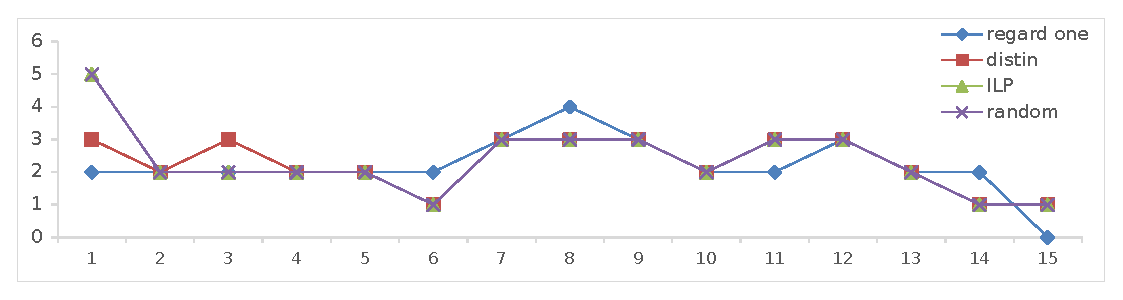
\includegraphics[width=2.64in]{accurate.eps}
}
\subfigure[Result of the number of identified sub-schemas of the MFS]{
  %  \rule{4cm}{3cm}
    \label{fig:22}
    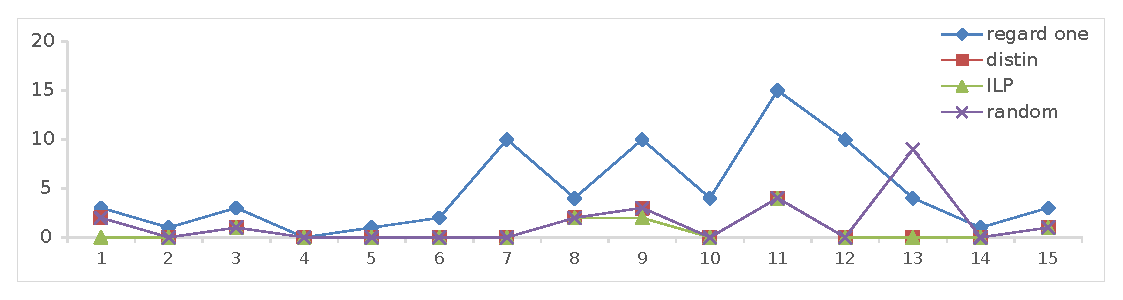
\includegraphics[width=2.64in]{sub.eps}
}
\subfigure[Result of the number of identified parent-schemas of the MFS]{
  %  \rule{4cm}{3cm}
    \label{fig:23}
    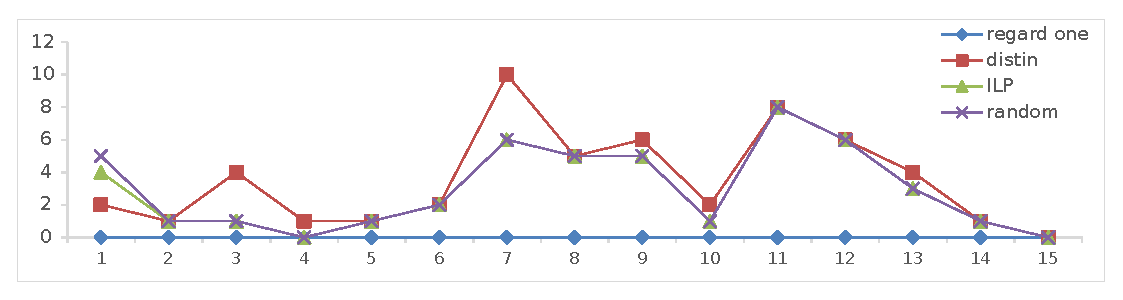
\includegraphics[width=2.64in]{parent.eps}
}
\subfigure[Result of the number of ignored MFS]{
  %  \rule{4cm}{3cm}
    \label{fig:24}
    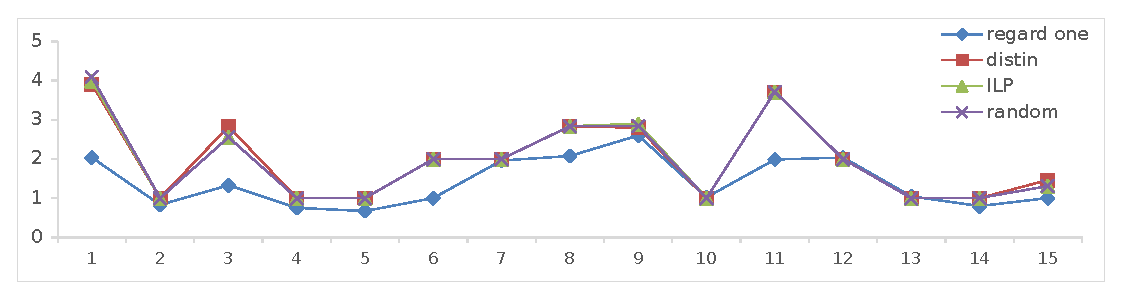
\includegraphics[width=2.64in]{ignore.eps}
}
\subfigure[Result of the number of identified irrelevant schemas of the MFS]{
  %  \rule{4cm}{3cm}
    \label{fig:25}
    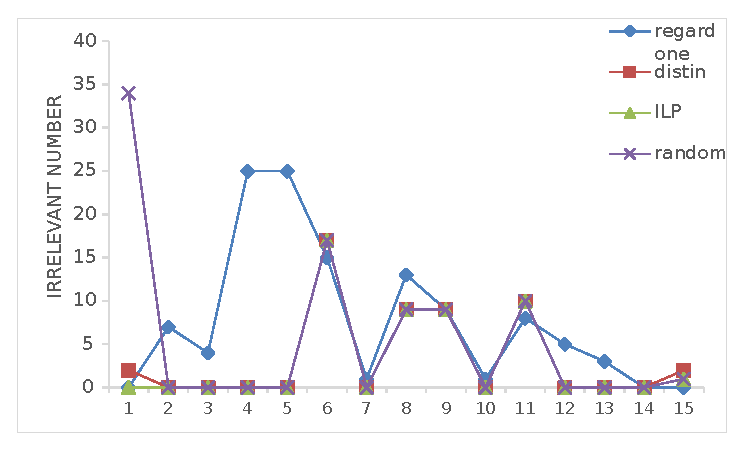
\includegraphics[width=2.64in]{irrelevant.eps}
}
\subfigure[The aggregative result for the five metrics]{
  %  \rule{4cm}{3cm}
    \label{fig:26}
    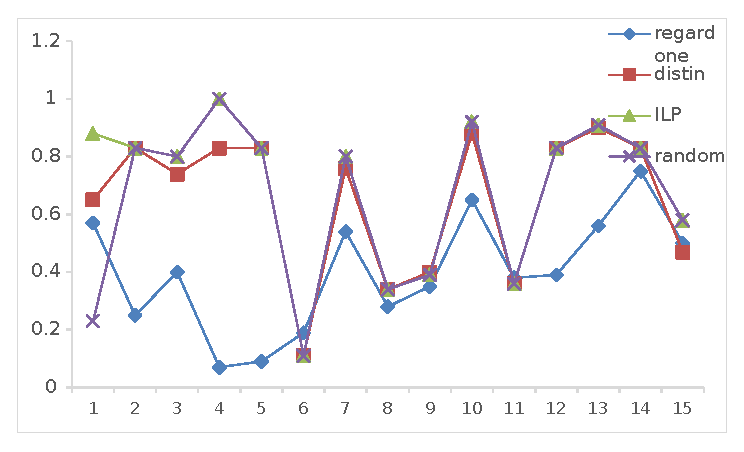
\includegraphics[width=2.64in]{overall.eps}
}
\subfigure[Needed test cases]{
  %  \rule{4cm}{3cm}
    \label{fig:27}
    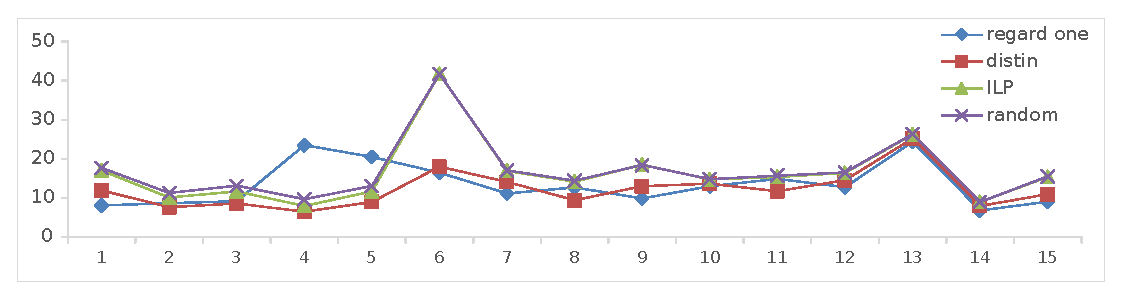
\includegraphics[width=2.64in]{testCases.eps}
}
\caption[Optional caption for list of figures]{Result of the evaluation of each appraoch}
\label{fig:comparetotraditional}
\end{figure*}


% Table generated by Excel2LaTeX from sheet 'Sheet1'

 Figure \ref{fig:comparetotraditional} depicts the results of the second case study. There are seven sub-figures in this figure, i.e., Figure \ref{fig:21} to Figure \ref{fig:27}. They indicate the results of : the number of accurate MFS each approach identified, the number of identified schemas which are the sub-schema / parent-schema of some prior MFS, the number of ignored prior MFS, the number of identified schemas which are irrelevant to all the prior MFS, the metric which gives the overall evaluation of each approach, and the extra test cases each algorithm needed, respectively. For each sub-figure, there are four polygonal lines in it, each of which shows the results for one of the four strategies: \emph{regarded as one failure}, \emph{distinguishing failures},  replacement strategy based on ILP searching,  replacement strategy based on randomly searching (The last one will be discussed in the next case study). Specifically, each point in the polygonal line indicates the specific result of a particular strategy for the corresponding testing object. For example at Figure \ref{fig:21}, the point marked with `$\blacklozenge$' at (1,2) indicates that the approach using \emph{regarded failures} identified 2 accurate MFS in the testing object--HSQLDB 2cr8. The raw data for this experiment can be found in Table \ref{evaluation_all} in the Appendix. Next we will discuss these results of these sub-figures.


\textbf{accurate number: }
Figure \ref{fig:21} shows the number of accurate schemas that each approach achieved. We can firstly find that there is no outstanding ones, i.e., not existing a strategy that can always perform better/worse than others in all these testing objects. This is because the accurate schemas is depend on the failure test cases it can figure out(either observed or predicted) as we discussed in the formal model in Section 3. Based on this, the two strategies \emph{regarded as one failure} and \emph{distinguishing failures} will both, in specific, \emph{regarded as one failure} will and \emph{distinguishing failures} will.

We can further find that for the two approaches, ILP and distin, have similar results about the number of identified accurate MFS. This can be easily understood, as the strategy ILP derived from the distin, which also make the failure distinguished with each other. And with some more refinement strategy. The

\textbf{sub number: }

Figure \ref{fig:22} depicts the results belong to this category. It is shows a more clear tend than \emph{accurate number}. We can easily find that the strategy \emph{regarded as one fault} performs the worst when compared to the ILP and distin approach. In fact, except for the fourth subject(JFlex 1.4.1), \emph{regarded as one failure} achieved more sub schemas than the other two strategies on all the remaining subjects. With respect to results for strategy \emph{regarded as one failure} and \emph{distinguishing failures}, we find that the result, i.e., \emph{regarded as one fault} will produce more sub schemas than \emph{distinguishing failures}, is as expected as discussed in section 4.

When compared  our approach ILP and the \emph{distinguishing failures}, we can learn that first the results are really similar to each other , and a step further we can find our approach perform a little better than that of \emph{distin} (at subject 1 and 9). We believe the little improvement is based on the fact our approach take the better test cases when encountering the not current fault condition, and the better test cases will get a good chance that the FCI will make better prediction of the failure test cases. So at last we can find that our approach can get less sub schemas.

\textbf{parent number: }
The result in Figure \ref{fig:23} shows that the \emph{regarded as one fault} performed better than the other two approaches. This is consistent with the formal analysis as this strategy the approach does not discard these test cases that may have masking effects, which make it less chances than \emph{distin} that will not make the MFS in the intersection area not be parent. Alougth we have predicted it can perform better than the other two approaches, we didn't expect it does not have even a parent schema than. In fact all these subjects is 0. It is interesting which drive us to deep insght what happened. And finally we get that .

Another observation about this metric is that similar to the sub number, when comparing ILP with distin, we can find that our approach can also perform a little better than distin. It is a evidence that the replacement process really improving the generated test cases quoality and make the predicetion better.

\textbf{ignore number: }

As respect to this metric, Figure \ref{fig:24} gives two viewpoints we can conclude: first, \emph{regarded as one failure} performs better than the other two approaches, this is also consistent with the formal analysis in section, because for the distin strategy, it will discard some important test cases which can directly make the MFS ignored; second, ILP performs better than the distin.

\textbf{irrelevant number: }
Figure \ref{fig:25} shows the results for this metric. We can firstly observed that except the point 1, 6, 9,11,14,15 that \emph{regarded as one failure} are have a similar result as ILP and distin, the remaining have a significance gap comparing to distin and ILP( \emph{regarded as one failure} normally identified have 10 to 20 more schemas that are irrelevant to the real MFS). This tell us \emph{regarded as one failure} have a poorer performance than the other two approaches at this metric. This result is also as expected as we in the formal anaysis section got that \emph{regarded as one failure} has more rules that can lead the schemas to be irrelevant ones.

As for the ILP and distin, we can still find ILP a little better than the distin. This can not be easily observed at this figure, but when we look at the raw data at Table \ref{evaluation_all}, we can find that ILP has on average identified 0.XXXX less irrelevant test cases.


%We can find that ILP and distin perfoms better than the \emph{regarded as one failure}, i.e., the schemas they identified to be irrelevant ones are less than that of the strategy \emph{regarded as one failure}.

\textbf{aggregative for the five metrics: }
When we composite these five metrics using the formula aforementioned and to comprehensive investigate the schemas that each approach get, we finally get Figure \ref{fig:26}. This figure gives a clear tend for the optimal and worse order of the approaches, i.e., ILP $>$ distin $>$ regard. In specific, for every subject except for the very similar ones such as 6, 8, 9, 11, the data shows this trend.

We can expect that ILP can peforms better than the distin because the ILP is acutally based on the distin, and do some refinement by getting higher quality test cases. As for distin better than regarded as one failure. We have not get it in the formal analysis, but however, we have a strong belief in that this is because this divde and conquer at least make the FCI approaches be more sensitive for the failures than the regarded as one failure.

\textbf{test cases: }
The above analysis, in a word, gives the comparable of the quality that each appraoch can result. This metric gives us the comparable ways about the cost, i.e., the extra test cases that each approach will generated. When we look at the Figure \ref{fig:27}, we can obviously find that the ILP will cost more test cases than distin and regard one. In specific, the gap between the ILP and distin and regard is ranged from about 2 to 5(except for the 6 subject, which exceeds 20), this is acceptable when comparing to the all the test cases that each test cases needed. This gap is expected as our ILP approaches needed to generate addtional test cases when some test cases are not satified the requirement.  When we looked back at the distin and regard one, there is no clear trend of which is better than another.

%
%We first observed that, the results of two traditional strategies, \emph{regarded as one failure} and \emph{distinguishing failures}, is consistent with the formal analysis in section 4. Specifically, the former has more sub-schemas of MFS than the latter for all the 15 subjects, and the latter has more parent-schemas of MFS than the former. For the `ignored MFS' metric, as we have executed all the failing test cases, we get 0 ignored MFS for all the approaches. So to evaluate this metric for these approaches, we record it for each test case at a time and take the average value as the result, which is listed in parentheses. We also found in most cases (except synthez 5 and synthez 6) that the approach with \emph{distinguish} strategy get more ignored MFS than the other, which also coincides with the formal analysis. And for the `irrelevant MFS', we found \emph{regarded as one failure} strategy in most cases got more `irrelevant MFS' than the other, which was also as expected.
%
%We then observed that our approach can perform better than the two traditional strategies. The advantages are shown in the more accurate MFS and less irrelevant schemas. Our approach also identified the least number of sub-schemas. As for the `parent-schema' metric, our approach performed better than `distinguishing failures' but not as well as `regarded as one failure'. This is because our strategy is based on the `distinguishing failures' strategy (the main difference is that our strategy filters the unsatisfied test cases). However, our approach is poor at the `ignored MFS' metric. The possible reason for this may be that the unsatisfied test cases we discard may contain some useful information about the MFS. Above all, our approach achieves the best performance compared with the other two strategies, which can be shown in the `overall' metric. The overall metric indicates that our approach performs better than `distinguishing failures' strategy, which is better than the `regarded as one failure' strategy.
%
%
%We further observed that, the extra cost (of generating test cases) for our approach is acceptable. In fact, when compared to the \emph{`distinguishing failures'} strategy, our approach needed an average of just 3 or 4 more test cases, and when compared to the \emph{`regarded as one failure'} strategy, our approach needed less test cases in some instances (JFlex 1.4.1, JFlex 1.4.2, synthez 3 and synthez 6). This is because the extra test cases the FCI needed lies in what the MFS is, the difference at the identified MFS for FCI approaches will make their needed test cases  differs greatly, so that the cost for replacing test cases in our approach may have little influence on the number of final test cases needed.



Above all, we can conclude about three points in this experiment, and which can be an answer for the \textbf{Q2}:

1)the results of distin and regard one are consistent with the formal analysis.

2)Considering the quality of the MFS each appraoch identified, we can find our approach can get the best, and then the distin.

3)Our approach need more test cases than ILP and distin, but which is acceptable.

 %the answer we got for \textbf{Q2} is that: our approach achieves better performance than two traditional strategies when handling masking effects at an acceptable % extra cost.

\subsection{Evaluating the ILP-based test case searching method}
The third empirical study aims to evaluate the efficiency of the ILP-based test case searching component in our approach. To conduct this study, we implemented an FCI approach which is also augmented by the \emph{replacing test cases} strategy, but the test case replacing process is by random.

%observe the performance of our approach and compare it with the result got by the traditional approaches. Our approach augments the three traditional FCI approaches with replacing test cases strategy described in Section 4.
%, and then we applied these augmented approaches to identify the failure-inducing combinations in the prepared subjects.

\subsubsection{Study setup}
The setup of this case study is based on the second case study, and uses the same SUT model as in Table \ref{testing_models}. Then, we apply the new random searching based FCI approach to identify the MFS in these prepared SUTs. To avoid the bias that comes from the randomness, we repeat the new approach 30 times to identify the MFS in each failing test case. We will compute the average additional test cases as well as other metrics listed in the previous section of the random-based approach.

% We will also take a look at how many scores can the new approach get when measuring the aforementioned metrics, as the same, we just compare the average scores with traditional ones.
%Additionally, comparisons between the augmented approaches and three traditional ones will be quantified.

\subsubsection{Results and discussion}
The evaluation of this random-based approach is also shown in Figure \ref{fig:comparetotraditional}, in which the polygonal line marked with  '$\times$' points in each sub-figure indicates this type of results. The raw data can be also found in the column 'R' of Table \ref{evaluation_all} in the appendix section.

Compared to our ILP-based approach, we can firstly observe that there is little distinction between them in terms of the metrics: accurate schemas, parent-schemas, sub-schemas, ignored schemas, irrelevant schemas ( for some particular cases the ILP-based approach performs slightly better, e.g., in Figure \ref{fig:22} for the first testing object, the ILP-based approach identified less sub schemas than that of the Random-based approach and in Figure \ref{fig:23} still for the first object the ILP -based approach identified less parent schemas than that of the random-based approach). The similarity quality of the identified MFS between this two approaches is conceivable as the two approaches both use the \emph{test case replacement} strategy, so when examining a schema, both of these two approaches may obtain the same result, although the test cases generated will be different.

Secondly, when considering the cost of each approach, we find the ILP-based approach performs better, which can reduce in the average to 1 or 2 test cases less compared to the random-based procedure. It is an evidence of our integer programming based searching technique can find a satisfied test case more rapidly than the random based one.

% there is significant improvement for augmented approaches in reducing the wrongly identified combinations. For instance, CTA approach in Fig \ref{fig:subfig6} only got 2 irrelevant combinations with replacing strategy, while the traditional two strategy got 5 and 19 irrelevant combinations respectively. And for FIC\_BS in Fig \ref{fig:subfig4} this comparison is 2 for replacing strategy, and 2 , 61 for two traditional strategies.

%Fig \ref{fig:subfigureExample2} presents the result of the last case study. The organization of this figure is similar to the second study. The bar in each column depicts the results of the augmented approaches, which is labelled as ``replacing strategy". We marked two additional points in each column which represent the result of \emph{regarded as one failure} and \emph{distinguish failures} strategy to get a comparison with the augmented approaches.

% We just added some information in the parentheses attached the value in each cell. This information display the  discrepancy between traditional ones. Notation '+' means promotions against traditional ones, while '-' indicates decrease. The value in parentheses has been normalized.

%\begin{figure*}[ht]
%\centering
%\subfigure[]{
%  %  \rule{4cm}{3cm}
%    \label{fig:subfig4}
%    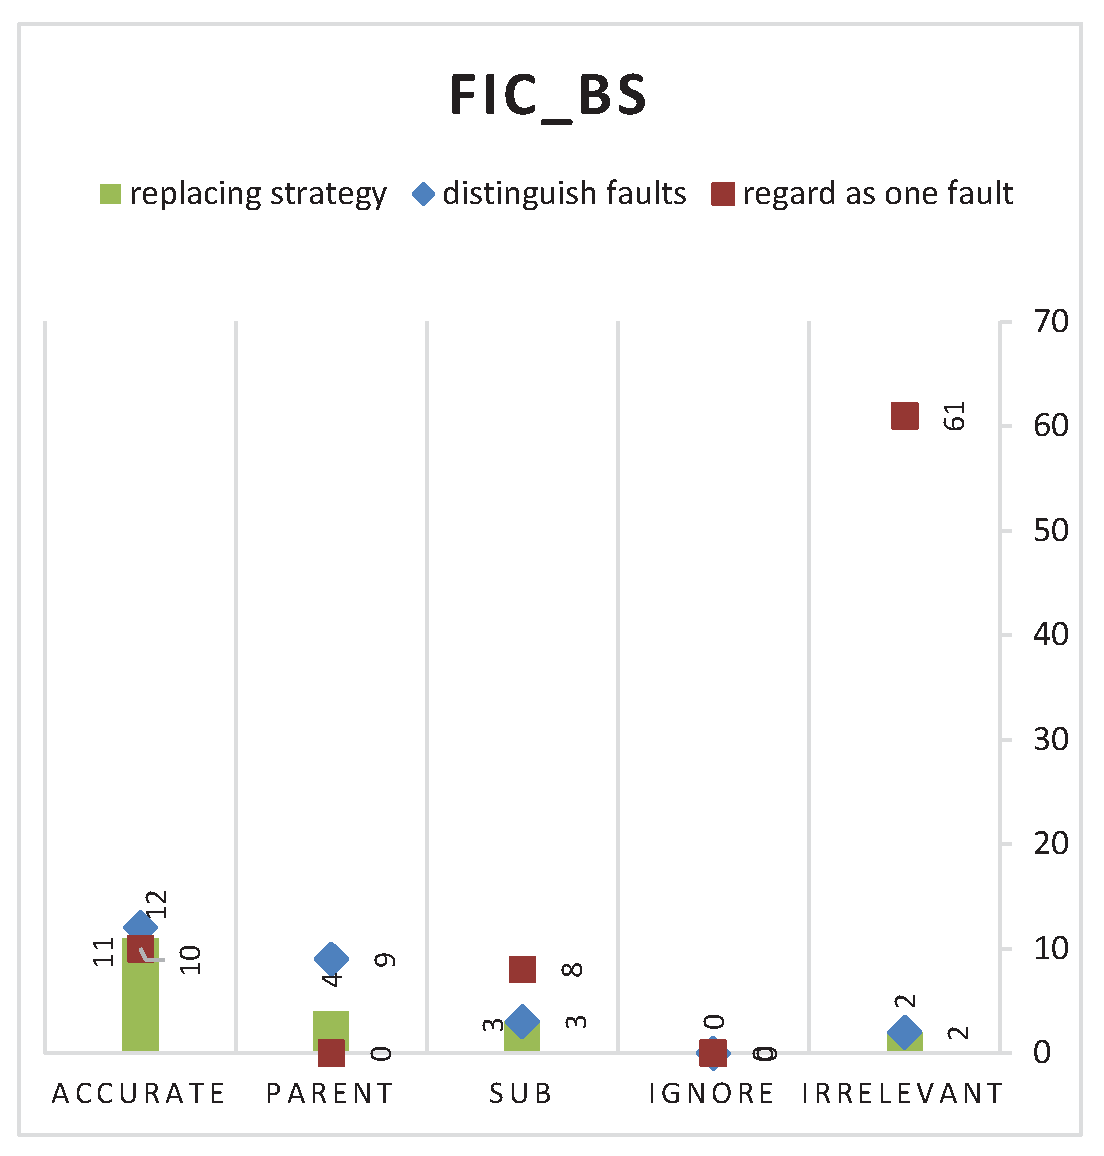
\includegraphics[width=2.21in]{FIC_BS_our.eps}
%}
%\subfigure[]{
%  %  \rule{4cm}{3cm}
%    \label{fig:subfig5}
%    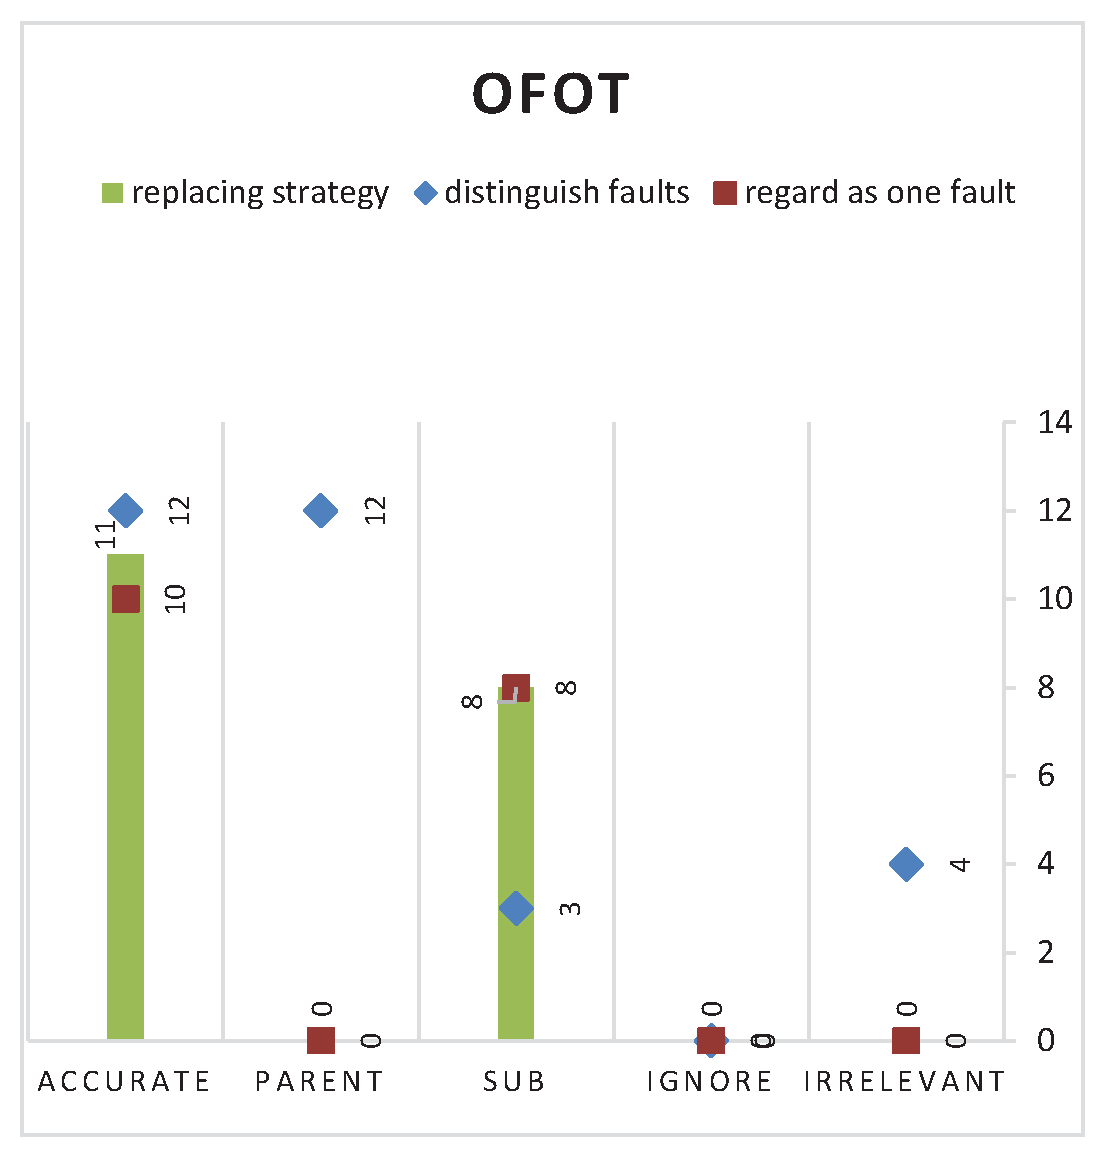
\includegraphics[width=2.21in]{OFOT_our.eps}
%}
%\subfigure[]{
%  %  \rule{4cm}{3cm}
%    \label{fig:subfig6}
%    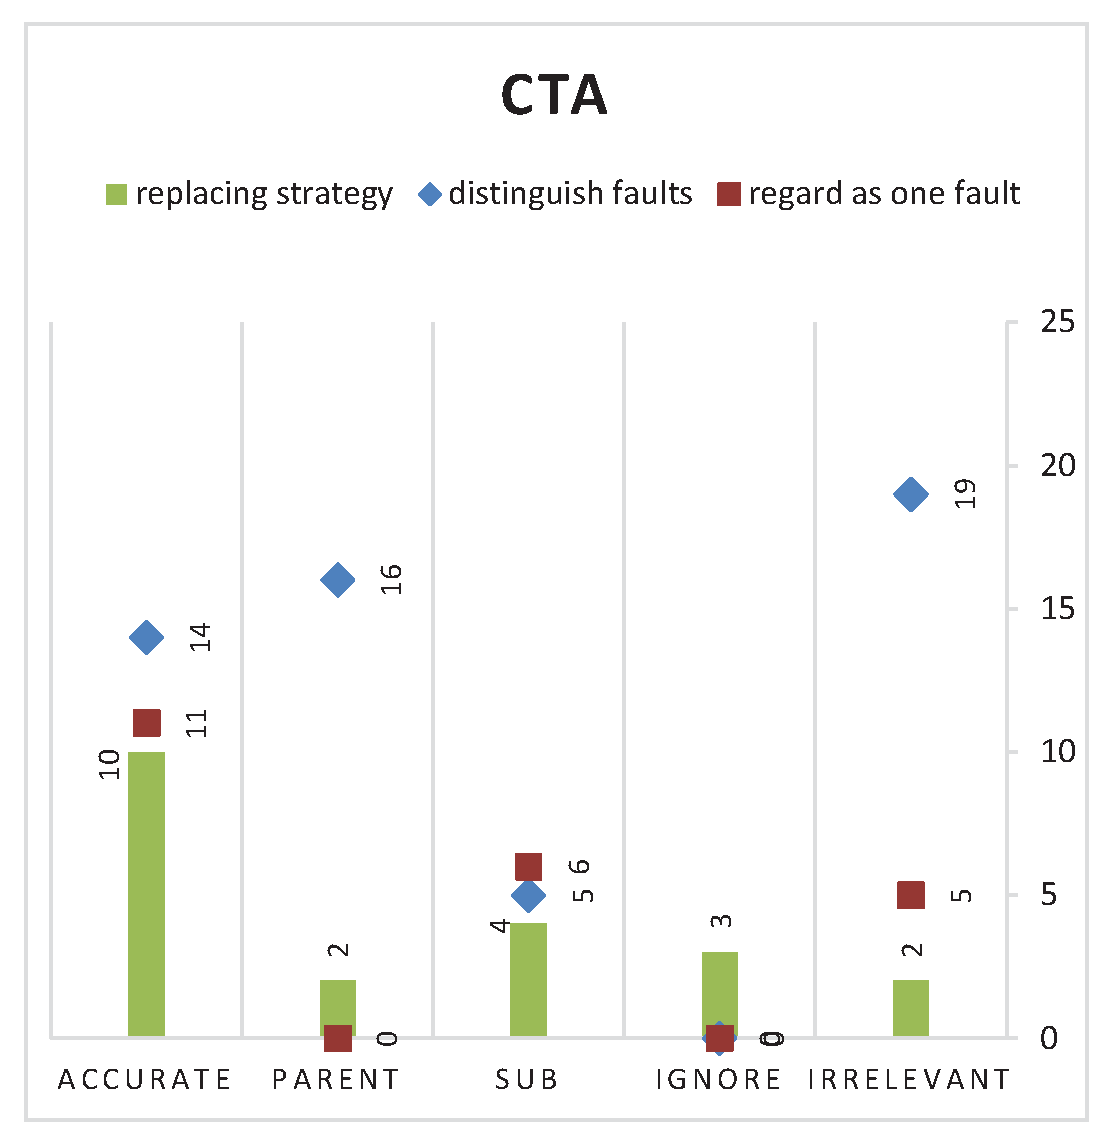
\includegraphics[width=2.21in]{CTA_our.eps}
%}
%\caption[Optional caption for list of figures]{Three approaches augmented with the replacing strategy}
%\label{fig:subfigureExample2}
%\end{figure*}




%Besides, the augmented approaches also get a good performance at limiting the number of sub combinations and parent combination. In effect, compared with \emph{distinguish failures} which is good at limiting sub combinations while producing more parent combinations and \emph{regard as one failure} which is the other way around, the augmented ones get a more balanced result. Specifically, for instance, in Fig \ref{fig:subfig4} for approach FIC\_BS, \emph{distinguish failures} strategy obtained 9 parent combinations while got 3 sub combinations. And for \emph{regard as one failure} strategy, it got none parent combination but attained 8 sub combinations. For the replacing strategy, it only identified 4 parent combinations, which smaller than \emph{distinguish failures} strategy, and obtained 3 sub combinations which is smaller than \emph{regard as one failure} strategy and equal to \emph{distinguish failures} strategy.
%
%Apart from these improvement, there is some slight decline for the augmented approaches in some specific situation. For example, we noted that for replacing strategy, it nearly got 2 less accurate combinations on average than traditional strategies, and ignored 1 more failure-inducing combinations on average than traditional ones.
% Further more it also that number of correctly identified combinations with replacing strategy slightly declines than traditional ones(about 2 less in average).

%As a compensation, however, We noted that the augment approaches got slightly . But promotions against traditional ones. In fact, there are 10 out of 14 cases that augment ones outperform traditional ones at the metric of "similarity", and 9 out of 14 cases that augment ones are better than traditional ones at the metric of "num diff". Additional, this promotion is distinct. As we can see, the best promotion for similarity is 0.9 and the best promotion for num diff is 0.7. Furthermore, the average performance promotion for similarity reached '+ 0.6' and this value reached '+ 0.5' for the num diff metric.

In summary, the answer for \textbf{Q3} is that: searching for a satisfied test case does have affect the performance of our approach, especially regarding the number of extra test cases, and the ILP-based test cases can handle the masking effects at a relatively smaller cost than the random-based approach.

%our approach do make the FCI approaches, to some extent, get better better performance at identifying failure-inducing combinations when facing masking effect between multiple failures.

%\subsection{Comparing with our previous work}
%The last empirical study aims to observe the performance of our approach and compare it with the result got by the traditional approaches. Our approach augments the three traditional FCI approaches with replacing test cases strategy described in Section 4.
%%, and then we applied these augmented approaches to identify the failure-inducing combinations in the prepared subjects.
%
%\subsubsection{Study setup}
%The setup of this case study is almost the same as the second case study. The difference is that the algorithms we choose are three augmented ones.
%
%%Additionally, comparisons between the augmented approaches and three traditional ones will be quantified.
%
%\subsubsection{Result and discussion}


%\subsection{Voting System}
%The last empirical study aims to observe the performance of our approach and compare it with the result got by the traditional approaches. Our approach augments the three traditional FCI approaches with replacing test cases strategy described in Section 4.
%%, and then we applied these augmented approaches to identify the failure-inducing combinations in the prepared subjects.
%
%\subsubsection{Study setup}
%The setup of this case study is almost the same as the second case study. The difference is that the algorithms we choose are three augmented ones.
%
%%Additionally, comparisons between the augmented approaches and three traditional ones will be quantified.
%
%\subsubsection{Result and discussion}
\subsection{Comparison with Feedback driven combinatorial testing}
The FDA-CIT \cite{yilmaz2013reducing} approach can handle masking effects so that the covering array it generates can cover all the t-way schemas without being masked by the MFS. There is an integrated FCI approach in the FDA-CIT, of which this FCI approach has two versions, i.e., ternary-class and multiple-class. In this paper, we use the multiple-class version for our comparative approach, as Yilmaz claims that the multiple-class version performs better than the former \cite{yilmaz2013reducing}.   %, the configuration options for J48, is .

\subsubsection{Study setup}
As the FCI approach of FDA-CIT use a post-analysis(classified tree) technique on given test cases, in this paper we fed the FDA-CIT the covering array as the input just as was done in the Yilmaz study \cite{yilmaz2013reducing}. The covering arrays we generated ranged from 2 to 4 ways. The covering array generating method we used is that contained in \cite{cohen2003augmenting}, as it can be easily extended with constraint dealing and seed injecting \cite{cohen2007interaction}, which is needed in the FDA-CIT process. As different test cases will influence the results of the characterization process, we generating 30 different 2 to 4 way covering arrays and fed them into the FDA-CIT. Then, we recorded the results of this approach, which consists of the metrics mentioned in the second case study.

Besides the FDA-CIT, we also applied our ILP-based approach to the generated covering array. Specifically, for each failing test case in the covering array, we separately applied our approach to identify the MFS in that case. In fact, we can reduce the number of extra test cases if we utilize the other test cases in the covering array \cite{li2012improved}), but we didn't utilize the information to simplify the experiment. We then merged all the test cases that our approach needed for each failing test case in the covering array, and we also merged other metrics listed in the second case study for each failing test case.

As our approach generated different test cases from the FDA-CIT, we also used the multiple-class FCI approach of FDA-CIT to characterize the MFS using the test cases generated by our approach, so that we could obtain a fair result with which to evaluate the FCI approach.
%with the same test cases generated by OFOT to get deterministic results. Additionally, the classified tree algorithms for CTA we chose is J48 implemented in Weka \cite{hall2009weka}. While all these approaches can help developers to isolate the failure-inducing combinations in failing test cases, in our recently studies on several open-source software, however, we found these approaches suffered from \emph{masking effects} of multiple failures in SUT. This effect was firstly introduced by Dumlu and Yilmaz in \cite{dumlu2011feedback}, in which they found that the masking effects in CT can make traditional covering array failed detecting some combinations and they proposed a feedback-driven approach to work around them. Their recent work \cite{yilmaz2013reducing} further empirically studied the impacts on the Failure-inducing Combinations Identifying(FCI) approach :  Classification Tree Approach(CTA)\cite{yilmaz2006covering},
\subsubsection{Result and discussion}
For each strength \emph{t}(ranged from 2 to 4), we conducted the experiment repeated 30 times for different covering arrays, we then recorded the average data(included accurate, sub, parent, irrelevant, ignored, overall and needed test cases) for the FDA-CIT, ILP-based approach, and FDA-CIT using our test cases (FDAs), respectively, for each subject. To conveniently and clearly visualize the result, we merged all the results of all the subjects for each approach and list them in Figure \ref{fig:comparefda}. The raw data which can show the result for each subject can be found in Table \ref{comparewithfda} in the appendix section. The result is organised the same as in Table \ref{evaluation_all}, except that we added a column \emph{t}  which indicates the strength of the covering array we generated for this experiment.

 \begin{figure*}[htbp]
\centering
\subfigure[Result for the 2-way covering array]{
  %  \rule{4cm}{3cm}
    \label{fig:31}
    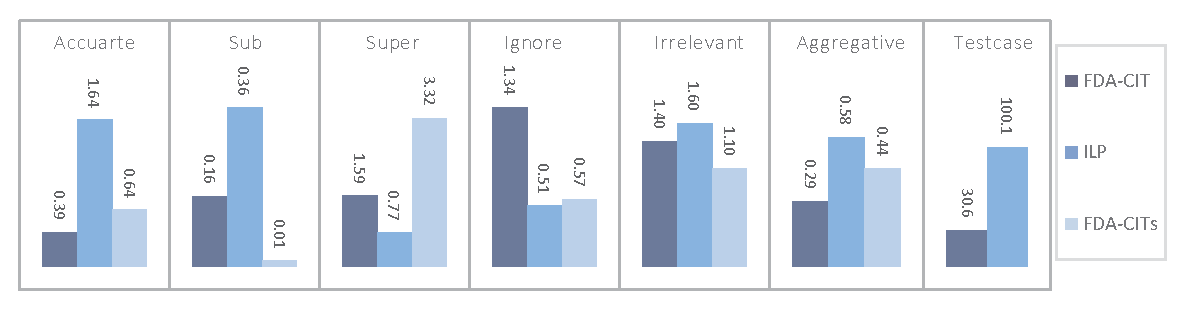
\includegraphics[width=5.4in]{2-way.eps}
}
\subfigure[Result for the 3-way covering array]{
  %  \rule{4cm}{3cm}
    \label{fig:32}
    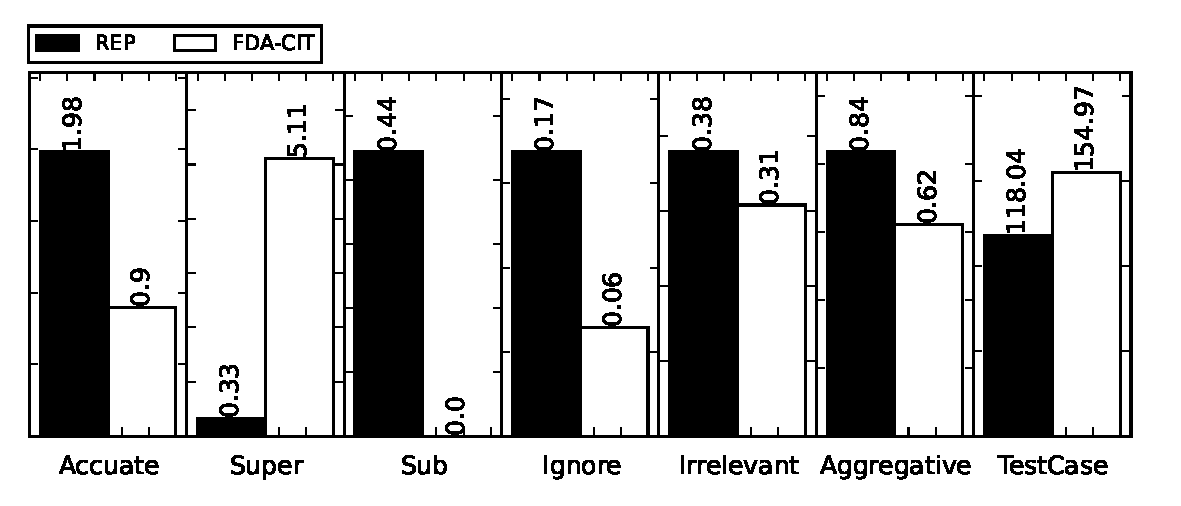
\includegraphics[width=5.4in]{3-way.eps}
}
\subfigure[Result of the 4-way covering array]{
  %  \rule{4cm}{3cm}
    \label{fig:33}
    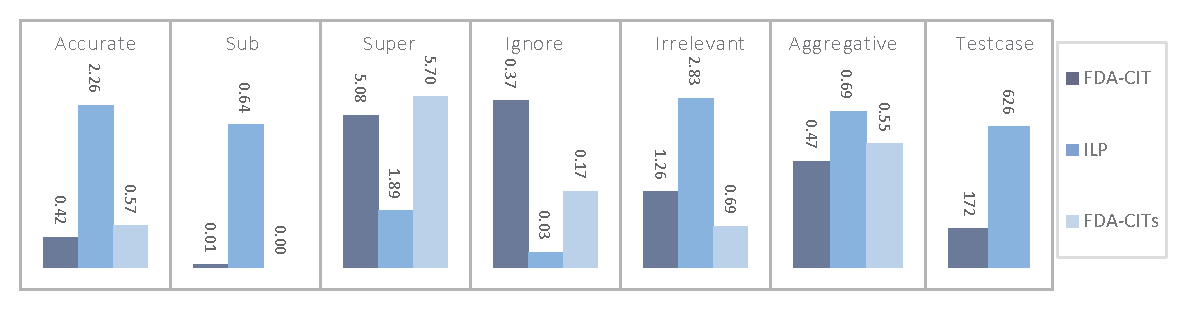
\includegraphics[width=5.4in]{4-way.eps}
}
\caption[Optional caption for list of figures]{Three approaches augmented with the replacing strategy}
\label{fig:comparefda}
\end{figure*}

At the first view of this figure, we can immediately get a conclusion that the trend that different approach  performs is never changed  with the change of the covering array strength. For example, focusing the metric \emph{ignored schemas}, we can find that for any of the t, there is always FDA $>$ FDA-s $>$ ILP. This observation tells us that different strength of the covering array doesn't have a affect on the performance rank of each approach, however, we can further observed that for a particular metric, the extent to which that the covering array has affect on the performance varies with the approach. Next we will detail these what these metrics have on the approaches and with the strength separately.


\textbf{Accurate number: }
From a over view, we can find that ILP $>$ FDA-s $>$ FDA. FDA-s $>$ FDA-s result is obvious, as it needs more test cases than the FDA, and more test cases means that the FCI approach can have a more rich observation and more precise predicts, i.e., the area B and C in Figure \ref{fig:fci_process} is larger. It is noted that the difference between these test cases is mainly because of the different FCI machinenory and , which will not be discussed here. Another view of this figure, we can find that ILP $>$ FDA-s, as this test cases is equal to each other, we can find that when using the test cases generated by the FIC\_BS, that the FIC\_BS will identified better than the classification-based approach. This is not a point to prove that the FIC\_BS is better than FDA, as when you cannot generate additional test cases, the classification tree is the most reasonable choice, and in that case FIC\_BS is not working.

Although the covering strength t doesn't affect the overal ranking performance of each approach, but how ever, it do affect the performance of each approach itself. As for the accurate metirc, we can find that with $t$ increasing, the ILP becomes better and better, in specific, when $t$ is 2, the accurate is 1.64. And the metric is 2.00 and 2.26 when t is 3 and 4, respectively. The more test cases, the richer and accurate is proved in this scenario. However, this is not the case of FDA. In fact, the trend that two FDA approaches is conversely with the increasing of the covering strength, i.e., the more test cases, the less number of accurate schemas it identified. This is strange, and as a potential reason, we believe that the classification tree approach may encounter the `overfit' problem, i.e., .


\textbf{Sub number: }
The sub metric in the overview is that ILP $>$ FDA $>$ FDA-s. When with increasing of the t, we can find the ILP sub increases, while FDA and FDA-s decrease.

For the overview rank, we can find, FDA and the FDA-s really have a better performance than ILP on limiting the number of schemas that are identified. This is mainly because the configuration we limit on the classification, i.e., the C4.5. A classification tree works as follows: it first choose a node as the most depart node, and next the follows.  A similar node tree is as Figure .  As the figure says.   With this in mind, we can the schemas used the classification tree are more tend to be parent schemas as it needs to using the leaf to index a schema, which may includes some unrelated parent nodes, e.g., the root nodes. Therefore, the parent schemas will be more than our ILP.

As for the FDA and FDA-s, we can find the FDA-s identify less sub schemas than FDA, this because the FDA-s use more test cases than FDA, and this lead a more detail partition for one node, and therefore, the sub schemas is less and less. This scene can also be observed as the increasing of the covering array strength, the test cases becomes more, so the sub schemas becomes less.

And for the ILP, we find that the increasing t, the increasing the sub schemas. This is consists with the formal model as the more test cases, the less the schemas.
%And for the increasing t, .


\textbf{Parent number: }
The parent metric in the overview is that FDA-s $>$ FDA $>$ ILP. When with the increasing of the t, all the approaches, ILP, FDA and FDA-s increases.

This is the just reverse scenario of the metric \emph{sub schemas}, and the result is just according to the analysis of the last result, so we will not discuss them for clear and simple.

\textbf{Ignore number: }
The ignore metric in the overview is that FDA $>$ FDA-s $>$ ILP. When with the increasing of the t, all the approaches decreases.

From this metirc, we can find that both the FDA and FDA-s miss more schemas than our ILP. We can further observe that the FDA miss more than FDA-s. It is a signal that our ILP can keep more useful information than FDA series.

Going to the formal model section, we can find the ignored schemas have too reasons: first, do not observe and predict some failing test cases, and schemas for these test cases do not have any relationship with these observed test cases, i.e., do not have any information of the original MFS; Second, the schemas that either not the parent or sub schemas of some MFS, i.e., the schemas may have part information of the MFS and have some irrelevant information of the MFS, e.g. (1 1 - 1) vs (1 1 1 -) , it less the third and more the fourth.  Then it can be explained that FDA have the most ignored schemas than FDA-s and ILP, beacuse it uses the least test cases, which can have a significantly impact on reducing the failing test cases that both can be observed and predicted.  This is also the reason the increasing t, the better that all these approaches identified less schemas.

As for the FDA-s and ILP, we can find our approach have a better performance, though their observed failing test cases are the same. This is mainly attributed to the difference of predicted failing test cases, which means that our ILP approach can have a better prediction than the FDA-s.

%For the second, i.e., all the approaches decrease the ignored schemas, is obvious, as the less the area we can ignore. Which have been discussed in the formal analysis.


\textbf{Irrelevant number: }
The irrelevant metric in the overview is that ILP $>$ FDA $>$ FDA-s. When with the increasing of the t, ILP increases, and FDA and FDA-s decreases.

For this metric, we can find that the FDA and FDA-s have a better performance than our ILP, which suggests that our appraoch may introduce more schemas that is no useful for determining the real MFS. This is somehow expected, as in a intuitive point, as our approach ignore less schemas, which may needs to try to get more schemas, and some of them may be irrelevant. In a deeper analysis, we can find the marchinary for the classification tree, though may have a tend to be parent schemas, can make the identified schemas be related to the real MFS.

%This metric is mainly because of the area that incorrectly predicate test cases.


\textbf{Aggregative for the five metrics: }
The aggregative metric for this overview is that ILP $>$ FDA-s $>$ FDA. When with the increasing of the t, all the approaches increases.

As we know, the aggregative gives the composite metric for the previous five metric, and comprehensively indicates the quality of the schemas that identified. Then for the result we can find that it is an evidence that the ILP performed better than the FDA and FDA-s at the quality of the schemas that is identified, i.e., our approach can support a better debugging aids for these schemas is more related to the real MFS.

It is to be expected that the more test cases, the more good quality the schemas that we can get. However, it is tradeoff for you to select a proper covering strength when considering the quality and the cost that need to be executed.

\textbf{Test cases: }
The overall test cases for the overview is that ILP $>$ FDA. (Noted, ILP is equal to FDA-s so we do not list them). When with the increasing of the t, all the approaches increases.

For the first, this is because of the difference of the approaches that we discussed. As the ILP approach is based on the FCI approach FCI\_BS (and of course, ILP can applied on other FCI approaches). Then from Table \ref{extra-testcases-complexisty}, we can learn that the FCI\_BS need to almost, it must be noted that this for one failing test case, the overall test cases for this approach is the covering array part add the part that the additional test cases for each failing test cases for this covering array. However, for FDA, it just need to generate several t-way covering array. So the difference between the appraoches ILP and FDA in our experiment if mainly attributed to the machinary of the FCI appraoch each approach adopts.

Above all, we can conclude about three points in this experiment, and which can be an answer for the \textbf{Q4}:

%1) FDA serial ����, and the ILP ���ӿ��ţ���˸����ʺϡ�

1)the general trend of the performance that each approach is never changed with the changing of the t.


2)Considering the quality of the MFS each approach identified, we can find our approach can get better than FDA and FDA-s, however, also using more test caes.

3)The increasing t a overall improvement for the quality but also increasing the test cases.

%
%From this result, we can first observe that in all the cases our ILP-based approach can more accurately identify the MFS and ignored less MFS than the FDA-CIT approach. For the metric `parent-schema', `sub-schema', and `irrelevant schemas', there are ups and downs on both sides. With respect to the `overall metric', we find our approach has a significant advantage over the FDA-CIT, but it also requires many more test cases than FDA-CIT.
%
%We note that, when applying the multiple-class FCI to characterize the MFS with the test cases that were generated using our approach, their `overall' metric is still not as good as our ILP-based approach, but may show some improvement over the original FDA-CIT.
%
%Another interesting observation is that overall performance in most cases is increasing with the $t$, which can be easily understood. More test cases will contain more information about the MFS, so that we can utilize them to identify the MFS more precisely.
%
%%
%%the t more, the result is more good, but there must be the over-fit problem, for example, for.
%%
%%it is because the improvement by the t-coverage is increasing quickly when the bug is 2-4 or large than 2, if the bug itself is less than 2 -4 , than the improvement is not obviously.
%
%So the answer for \textbf{Q4} is that: our approach can achieved a more precise result for the MFS, and the FDA-CIT can perform the identifying process using a small amount extra test cases. Both of these two approaches have their ups and downs, choosing which approach in practice will depend on the specific scenario you test.
%% if you want to get a more precise result and more helpful test cases generating supply, you should choose our approach, however if you are limited to the test cases execution, you can choose the feedback driven.
%% but if
\subsection{Threats to validity}

As we previous metioned, the masking effects can be having a complicated relationship, not the directly linear about multiple failures. I.e., failure a can mask the failure b, failure b can mask a . and failure c can mask failure c. Even worse, two failures can mask each other. When such scenorias happened, we need to recoonsruct the formal model of the schemas that when can be either be.  as the condition will significantly completed the relationships between the failures and schemas.

\subsubsection{internal threats}
There are several threats to the validity for these empirical studies. First, we have only surveyed two types of open-source software with five different versions, of which the program scale is medium-sized. This may impact the generality of our observations. Although we believe it is quite possibly a common phenomenon in most software that contains multiple failures which can mask each other, we need to investigate more software to support our belief.

The second threat comes from the input model we built. As we focused on the options related to the perfect combinations and only augmented it with some noise options, there is a chance we will get different results if we choose other noise options. More options needed to be tested to see whether our result is common or just appears in some particular input models.
\subsubsection{external threats}


The third threat is that we just evaluated one FCI approach -- FIC\_BS \cite{zhang2011characterizing}, so further works needed to examine more algorithms in this field to obtain a more general result.

Another important discussion is that our approach is based on the fact that the different errors can be distinguished in some way, such as, the bug exception traces or the like. If we cannot distinguish them, or too costly to identify the difference of two faults, then, our approach does not work. We believe in such a way the only thing to do is to try to fix some bugs you believe, and then try if there is any faults remained.

\section{related works}

Shi and Nie presented an approach for failure revealing and failure diagnosis in CT \cite{shi2005software}, which first tests the SUT with a covering array, then reduces the value schemas contained in the failing test case by eliminating those appearing in the passing test cases. If the failure-causing schema is found in the reduced schema set, failure diagnosis is completed with the identification of the specific input values which caused the failure; otherwise, a further test suite based on SOFOT is developed for each failing test cases,testing is repeated, and the schema set is then further reduced, until no more failures are found or the failure is located. Based on this work, Wang proposed an AIFL approach which extended the SOFOT process by adaptively mutating factors in the original failing test cases in each iteration to characterize failure-inducing combinations\cite{wang2010adaptive}.

Nie et al. introduced the notion of Minimal Failure-causing Schema(MFS) and proposed the OFOT approach which is an extension of SOFOT that can isolate the MFS in SUT\cite{nie2011minimal}. The approach mutates one value with different values for that parameter, hence generating a group of additional test cases each time to be executed. Compared with SOFOT, this approach  strengthen the validation of the factor under analysis and also can detect the newly imported faulty combinations.

Delta debugging proposed by Zeller \cite{zeller2002simplifying} is an adaptive divide-and-conquer approach to locate interaction failure. It is very efficient and has been applied in real software environment. Zhang et al. also proposed a similar approach that can efficiently identify the failure-inducing combinations that has no overlapped part \cite{zhang2011characterizing}. Later, Li improved the delta-debugging based failure-inducing combination by exploiting useful information in the executed covering array\cite{li2012improved}.

Colbourn and McClary proposed a non-adaptive method \cite{colbourn2008locating}. Their approach extends a covering array to the locating array to detect and locate interaction failures. C. Martinez proposed two adaptive algorithms. The first one requires safe value as the assumption and the second one removes the assumption when the number of values of each parameter is equal to 2\cite{martinez2008algorithms,martinez2009locating}. Their algorithms focus on identifying faulty tuples that have no more than 2 parameters.

Ghandehari et al. defined the suspiciousness of tuple and suspiciousness of the environment of a tuple\cite{ghandehari2012identifying}. Based on this, they rank the possible tuples and generate the test configurations. They further utilized the test cases generated from the inducing combination to locate the failures inside the source code\cite{ghandehari2013fault}.

Yilmaz proposed a machine learning method to identify inducing combinations from a combinatorial testing set \cite{yilmaz2006covering}. They constructed a classification tree to analyze the covering arrays and detect potential faulty combinations. Beside this, Fouch{\'e} \cite{fouche2009incremental} and Shakya \cite{shakya2012isolating} made some improvements in identifying failure-inducing combinations based on Yilmaz's work.

Our previous work \cite{niu2013identifying} proposed an approach that utilizes the tuple relationship tree to isolate the failure-inducing combinations in a failing test case. One novelty of this approach is that it can identify the overlapped faulty combinations. This work also alleviates the problem of introducing new failure-inducing combinations in additional test cases.

In addition to the studies that aim at identifying the failure-inducing combinations in test cases, there are others that focus on working around the masking effects.

With having known masking effects in prior, Cohen \cite{cohen2007exploiting,cohen2007interaction,cohen2008constructing} studied the impact of the masking effects that render some generated test cases invalid in CT. They also proposed an approach that integrates the incremental SAT solver with the covering arrays's generation algorithm to avoid masking effects. Further study was conducted \cite{petke2013efficiency}to show that with considering constrains, higher-strength covering arrays with early failure detection are practical. Besides, additional works that aim to study the impacts of constraints for CT were as follows:  \cite{garvin2011evaluating,bryce2006prioritized,calvagna2008logic,grindal2006handling,yilmaz2013test}. %These approaches use some rules or to avoid these invalidated test cases to improve the efficiency when examine the test cases.

Chen et al. addressed the issues of shielding parameters in combinatorial testing and proposed the Mixed Covering Array with Shielding Parameters (MCAS) to solve the problem caused by shielding parameters\cite{chen2010combinatorial}. The shielding parameters can disable some parameter values to expose additional interaction errors, which can be regarded as a special case of masking effects.

Dumlu and Yilmaz proposed a feedback-driven approach to work around the masking effects\cite{dumlu2011feedback}. Specifically, they first used classification tree approach to classify the possible failure-inducing combinations and then eliminate them and generate new test cases to detect possible masked interaction in the next iteration. They further extended their work \cite{yilmaz2013reducing} by proposing a multiple-class CTA approach to distinguishing failures in SUT. In addition, they empirically studied the impacts on both ternary-class and multiple-class CTA approaches.

Our work differs from these mainly in that we formally studied the masking effects on FCI approaches and further proposed a divide-and-conquer strategy to alleviate this impact.

\section{Conclusions}
Masking effects of multiple failures in SUT can bias the results of traditional failure-inducing combinations identifying approaches. In this paper, we formally analysed the impact of masking effects on FCI approaches and showed that the two traditional strategies, i.e., \emph{regarded as one fault} and \emph{distinguishing failures}, are both inefficient in handling such impact. We further presented a divide-and-conquer strategy for FCI approaches to alleviate such impact.

%This strategy separately handle each failure in SUT, and for a particular failure, it will discard these test cases that trigger failures different from the one under analysis and only keep those that either pass or trigger the expected failure. Additional test cases for compensation will be generated after discarding unsatisfied test cases.

In our empirical studies, we extended FCI approach -- FIC\_BS\cite{zhang2011characterizing} with our strategy. The comparison between our approach and traditional approaches was performed on several kinds of open-source software. The results indicated that our strategy assists the traditional FCI approach in achieving better performance when facing masking effects in SUT. We also empirically evaluated the efficiency of the test case searching component by comparing it with the random searching based FCI approach. The results showed that the ILP-based test case searching method can perform much more efficiently. Last, we compared our approach with existing technique for handling masking effects -- FDA-CIT\cite{yilmaz2013reducing}, and observed that our approach achieved a more precise result which can support better debugging aids, though our approach generated more test cases than FDA-CIT.

As for the future work, we need to do more empirical studies to make our conclusions more general. Our current experiments focus on middle-sized software. We would like to extend our approach to more complicated, large-scaled testing scenarios. Another promising work in the future is to combine the white-box testing technique to facilitate obtaining more accurate results from the FCI approaches when handling masking effects. We believe that figuring out the failure levels of different bugs through the white-box testing technique is helpful to reduce misjudgement in the failure-inducing combinations identifying process. And last, because the extent to which the FCI suffers from masking effects varies with different algorithms, a combination of different FCI approaches would be desired in the future to further improve identifying MFS for multiple failures.



% Start of "Sample References" section

%\section{Typical references in new ACM Reference Format}
%%A paginated journal article \cite{Abril07}, an enumerated
%%journal article \cite{Cohen07}, a reference to an entire issue \cite{JCohen96},
%%a monograph (whole book) \cite{Kosiur01}, a monograph/whole book in a series (see 2a in spec. document)
%%\cite{Harel79}, a divisible-book such as an anthology or compilation \cite{Editor00}
%%followed by the same example, however we only output the series if the volume number is given
%%\cite{Editor00a} (so Editor00a's series should NOT be present since it has no vol. no.),
%%a chapter in a divisible book \cite{Spector90}, a chapter in a divisible book
%%in a series \cite{Douglass98}, a multi-volume work as book \cite{Knuth97},
%%an article in a proceedings (of a conference, symposium, workshop for example)
%%(paginated proceedings article) \cite{Andler79}, a proceedings article
%%with all possible elements \cite{Smith10}, an example of an enumerated
%%proceedings article \cite{VanGundy07},
%%an informally published work \cite{Harel78}, a doctoral dissertation \cite{Clarkson85},
%%a master's thesis: \cite{anisi03}, an online document / world wide web resource \cite{Thornburg01}, \cite{Ablamowicz07},
%%\cite{Poker06}, a video game (Case 1) \cite{Obama08} and (Case 2) \cite{Novak03}
%%and \cite{Lee05} and (Case 3) a patent \cite{JoeScientist001},
%%work accepted for publication \cite{rous08}, 'YYYYb'-test for prolific author
%%\cite{SaeediMEJ10} and \cite{SaeediJETC10}. Other cites might contain
%%'duplicate' DOI and URLs (some SIAM articles) \cite{Kirschmer:2010:AEI:1958016.1958018}.
%%Boris / Barbara Beeton: multi-volume works as books
%%\cite{MR781536} and \cite{MR781537}.
%
%% Appendix
%\appendix
%\section*{APPENDIX}
%\setcounter{section}{1}
%
%
%\appendixhead{ZHOU}

% Acknowledgments
%\begin{acks}
%The authors would like to thank Dr. Maura Turolla of Telecom
%Italia for providing specifications about the application scenario.
%\end{acks}

% Bibliography
\bibliographystyle{ACM-Reference-Format-Journals}
\bibliography{acmsmall-sample-bibfile}
                             % Sample .bib file with references that match those in
                             % the 'Specifications Document (V1.5)' as well containing
                             % 'legacy' bibs and bibs with 'alternate codings'.
                             % Gerry Murray - March 2012

% History dates
%\received{February 2007}{March 2009}{June 2009}

% Electronic Appendix
\elecappendix

\medskip

\section{The detail of the experiments}


\begin{table}[htbp]
\begin{threeparttable}
\tbl{Result of the evaluation of each appraoch\label{evaluation_all}}{
\setlength\tabcolsep{2pt}
 \begin{tabular}{|l|llll|llll|llll|llll|llll|llll|llll}
\hline
\textbf{Subject} & \multicolumn{4}{l|}{\textbf{accurate}} & \multicolumn{4}{l|}{\textbf{sub}} & \multicolumn{4}{l|}{\textbf{parent}} & \multicolumn{4}{l|}{\textbf{ignore}}  & \multicolumn{4}{l|}{\textbf{irrelevant}} & \multicolumn{4}{l|}{\textbf{overall}} & \multicolumn{4}{l|}{\textbf{test cases}}           \\ \hline
                 & O \tnote{1}        & D  \tnote{2}      & I   \tnote{3}     & R  \tnote{4}      & O       & D      & I      & R     & O       & D        & I      & R      & O       & D       & I       & R       & O        & D        & I        & R       & O       & D       & I       & R       & O     & D     & I     & \multicolumn{1}{l|}{R}     \\
HSQLDB 2cr8      & 2        & 3       & 5       & 5       & 3       & 2      & 0      & 2     & 0       & 2        & 4      & 5      & 0(2.04) & 0(3.91) & 0(4.0)  & 0(4.1)  & 0        & 2        & 0        & 34      & 0.57    & 0.65    & 0.88    & 0.23    & 8.125 & 11.92 & 17    & \multicolumn{1}{l|}{17.72} \\
HSQLDB 2.2.5     & 2        & 2       & 2       & 2       & 1       & 0      & 0      & 0     & 0       & 1        & 1      & 1      & 0(0.83) & 0(1.0)  & 0(1.0)  & 0(1.0)  & 7        & 0        & 0        & 0       & 0.25    & 0.83    & 0.83    & 0.83    & 8.67  & 7.67  & 10.17 & \multicolumn{1}{l|}{11.3}  \\
HSQLDB 2.2.9     & 2        & 3       & 2       & 2       & 3       & 1      & 1      & 1     & 0       & 4        & 1      & 1      & 0(1.33) & 0(2.83) & 0(2.56) & 0(2.56) & 4        & 0        & 0        & 0       & 0.4     & 0.74    & 0.8     & 0.8     & 9.167 & 8.61  & 11.72 & \multicolumn{1}{l|}{13.14} \\
JFlex 1.4.1      & 2        & 2       & 2       & 2       & 0       & 0      & 0      & 0     & 0       & 1        & 0      & 0      & 0(0.75) & 0(1.0)  & 0(1.0)  & 0(1.0)  & 25       & 0        & 0        & 0       & 0.07    & 0.83    & 1       & 1       & 23.5  & 6.5   & 8     & \multicolumn{1}{l|}{9.68}  \\
JFlex 1.4.2      & 2        & 2       & 2       & 2       & 1       & 0      & 0      & 0     & 0       & 1        & 1      & 1      & 0(0.67) & 0(1.0)  & 0(1.0)  & 0(1.0)  & 25       & 0        & 0        & 0       & 0.09    & 0.83    & 0.83    & 0.83    & 20.5  & 9     & 11.67 & \multicolumn{1}{l|}{13.12} \\
synthez 1        & 2        & 1       & 1       & 1       & 2       & 0      & 0      & 0     & 0       & 2        & 2      & 2      & 0(1.0)  & 0(2.0)  & 0(2.0)  & 0(2.0)  & 15       & 17       & 17       & 17      & 0.19    & 0.11    & 0.11    & 0.11    & 16.5  & 18    & 41.75 & \multicolumn{1}{l|}{41.75} \\
synthez 2        & 3        & 3       & 3       & 3       & 10      & 0      & 0      & 0     & 0       & 10       & 6      & 6      & 0(1.96) & 0(2.0)  & 0(2.0)  & 0(2.0)  & 1        & 0        & 0        & 0       & 0.54    & 0.76    & 0.8     & 0.8     & 11.19 & 14.12 & 16.96 & \multicolumn{1}{l|}{17.08} \\
synthez 3        & 4        & 3       & 3       & 3       & 4       & 2      & 2      & 2     & 0       & 5        & 5      & 5      & 0(2.08) & 0(2.84) & 0(2.84) & 0(2.84) & 13       & 9        & 9        & 9       & 0.28    & 0.34    & 0.34    & 0.34    & 12.73 & 9.46  & 14.18 & \multicolumn{1}{l|}{14.44} \\
synthez 4        & 3        & 3       & 3       & 3       & 10      & 3      & 2      & 3     & 0       & 6        & 5      & 5      & 0(2.6)  & 0(2.8)  & 0(2.9)  & 0(2.85) & 9        & 9        & 9        & 9       & 0.35    & 0.4     & 0.39    & 0.39    & 9.91  & 13.02 & 18.55 & \multicolumn{1}{l|}{18.45} \\
synthez 5        & 2        & 2       & 2       & 2       & 4       & 0      & 0      & 0     & 0       & 2        & 1      & 1      & 0(1.02) & 0(1.0)  & 0(1.0)  & 0(1.0)  & 1        & 0        & 0        & 0       & 0.65    & 0.88    & 0.92    & 0.92    & 13.04 & 13.7  & 14.77 & \multicolumn{1}{l|}{14.84} \\
synthez 6        & 2        & 3       & 3       & 3       & 15      & 4      & 4      & 4     & 0       & 8        & 8      & 8      & 0(1.99) & 0(3.72) & 0(3.72) & 0(3.72) & 8        & 10       & 10       & 10      & 0.38    & 0.36    & 0.36    & 0.36    & 14.91 & 11.75 & 15.37 & \multicolumn{1}{l|}{15.71} \\
synthez 7        & 3        & 3       & 3       & 3       & 10      & 0      & 0      & 0     & 0       & 6        & 6      & 6      & 0(2.04) & 0(2.0)  & 0(2.0)  & 0(2.0)  & 5        & 0        & 0        & 0       & 0.39    & 0.83    & 0.83    & 0.83    & 12.77 & 14.59 & 16.44 & \multicolumn{1}{l|}{16.53} \\
synthez 8        & 2        & 2       & 2       & 2       & 4       & 0      & 0      & 9     & 0       & 4        & 3      & 3      & 0(1.05) & 0(1.0)  & 0(1.0)  & 0(1.0)  & 3        & 0        & 0        & 0       & 0.56    & 0.9     & 0.91    & 0.91    & 24.45 & 25.25 & 26.27 & \multicolumn{1}{l|}{26.37} \\
synthez 9        & 2        & 1       & 1       & 1       & 1       & 0      & 0      & 0     & 0       & 1        & 1      & 1      & 0(0.8)  & 0(1.0)  & 0(1.0)  & 0(1.0)  & 0        & 0        & 0        & 0       & 0.75    & 0.83    & 0.83    & 0.83    & 6.8   & 8     & 9     & \multicolumn{1}{l|}{9}     \\
synthez 10       & 0        & 1       & 1       & 1       & 3       & 1      & 1      & 1     & 0       & 0        & 0      & 0      & 0(1.0)  & 0(1.46) & 0(1.31) & 0(1.31) & 0        & 2        & 1        & 1       & 0.5     & 0.47    & 0.58    & 0.58    & 9.08  & 11    & 15.38 & \multicolumn{1}{l|}{15.53} \\ \hline
\end{tabular}
    }

     \begin{tablenotes}
        \footnotesize
        \item[1] $O$ is for the strategy \emph{regarded as one failure}.
        \item[2] $D$ is for the strategy \emph{distinguishing failures}.
        \item[3] $I$ is for the replacement strategy based on ILP searching.
        \item[4] $R$ is for the replacement strategy based on randomly searching.
      \end{tablenotes}
%  \label{tab:addlabel}%
\end{threeparttable}
\end{table}%

\begin{table}[htbp]
\begin{threeparttable}
\tbl{Comparison with FDA-CIT\label{comparewithfda}}{
\setlength{\tabcolsep}{3pt}
\begin{tabular}{|l|l|lll|lll|lll|lll|lll|lll|lll}
\hline
\textbf{Subject} & \textbf{} & \multicolumn{3}{l|}{\textbf{accurate}} & \multicolumn{3}{l|}{\textbf{sub}} & \multicolumn{3}{l|}{\textbf{parent}} & \multicolumn{3}{l|}{\textbf{ignore}} & \multicolumn{3}{l|}{\textbf{irrelevant}} & \multicolumn{3}{l|}{\textbf{overall}} & \multicolumn{3}{l|}{\textbf{test cases}}      \\ \hline
                 & t         & F    \tnote{1}       & I     \tnote{2}      & Fs      \tnote{3}   & F         & I         & Fs        & F          & I          & F          & F          & I          & Fs         & F           & I            & Fs          & F           & I          & Fs         & F     & I      & \multicolumn{1}{l|}{Fs}     \\
HSQL2cr8         & 2         & 0.17        & 2.27        & 1.57       & 0.57      & 0         & 0         & 0.17       & 0.4        & 2.17       & 3.87       & 2.3        & 2          & 2.53        & 0            & 1.97        & 0.12        & 0.51       & 0.39       & 23.6  & 70.1   & \multicolumn{1}{l|}{70.1}   \\
                 & 3         & 1.47        & 3.67        & 1          & 0         & 0         & 0         & 4.67       & 2          & 6.07       & 0.63       & 0.3        & 0.17       & 3           & 0            & 1.47        & 0.51        & 0.87       & 0.6        & 76.6  & 241.8  & \multicolumn{1}{l|}{241.8}  \\
                 & 4         & 0.83        & 4.8         & 1          & 0         & 0         & 0         & 9.03       & 3.37       & 8          & 0          & 0          & 0          & 0.97        & 0            & 0           & 0.65        & 0.9        & 0.71       & 183.5 & 606.6  & \multicolumn{1}{l|}{606.6}  \\
HSQL2.2.5        & 2         & 1           & 1.97        & 0.37       & 0         & 0         & 0         & 2.4        & 0.73       & 3.8        & 0.4        & 0          & 0          & 1.4         & 0            & 0.1         & 0.38        & 0.87       & 0.56       & 26.7  & 68.8   & \multicolumn{1}{l|}{68.8}   \\
                 & 3         & 0           & 2           & 0.4        & 0         & 0         & 0         & 5          & 1          & 3.8        & 0          & 0          & 0          & 0           & 0            & 0           & 0.52        & 0.83       & 0.56       & 67    & 202.4  & \multicolumn{1}{l|}{202.4}  \\
                 & 4         & 0           & 2           & 0.33       & 0         & 0         & 0         & 5          & 1          & 4          & 0          & 0          & 0          & 0           & 0            & 0           & 0.53        & 0.83       & 0.56       & 130.1 & 503.3  & \multicolumn{1}{l|}{503.3}  \\
HSQL2.2.9        & 2         & 0.9         & 1.77        & 0.9        & 0         & 0.77      & 0         & 1.47       & 0.47       & 6.8        & 1.93       & 0.53       & 0          & 2.37        & 0            & 0.2         & 0.28        & 0.72       & 0.58       & 29.2  & 78.3   & \multicolumn{1}{l|}{78.3}   \\
                 & 3         & 1           & 2           & 0.83       & 0         & 1         & 0         & 5.13       & 0.93       & 7.1        & 0.2        & 0          & 0          & 0.1         & 0            & 0           & 0.61        & 0.8        & 0.61       & 72.8  & 221.7  & \multicolumn{1}{l|}{221.7}  \\
                 & 4         & 1           & 2           & 1          & 0         & 1         & 0         & 5.87       & 1          & 6.7        & 0          & 0          & 0          & 0           & 0            & 0           & 0.64        & 0.8        & 0.62       & 129.8 & 560.3  & \multicolumn{1}{l|}{560.3}  \\
JFlex 1.4.1      & 2         & 0           & 2           & 0          & 0         & 0         & 0         & 4.03       & 0          & 4          & 0          & 0          & 0          & 0           & 0            & 0           & 0.49        & 1          & 0.5        & 30.5  & 87.3   & \multicolumn{1}{l|}{87.3}   \\
                 & 3         & 0           & 2           & 0          & 0         & 0         & 0         & 4          & 0          & 0          & 0          & 0          & 4          & 0           & 0            & 0           & 0.5         & 1          & 0.5        & 73.4  & 269.2  & \multicolumn{1}{l|}{269.2}  \\
                 & 4         & 0           & 2           & 0          & 0         & 0         & 0         & 4          & 0          & 0          & 0          & 0          & 0          & 0           & 0            & 0           & 0.5         & 1          & 0.5        & 190.6 & 724.7  & \multicolumn{1}{l|}{724.7}  \\
JFlex 1.4.2      & 2         & 0.3         & 1.97        & 0.93       & 0         & 0         & 0         & 3.6        & 1          & 2.16       & 0.03       & 0          & 0          & 0.63        & 0            & 0           & 0.5         & 0.83       & 0.62       & 34.3  & 106.9  & \multicolumn{1}{l|}{106.9}  \\
                 & 3         & 0           & 2           & 0.97       & 0         & 0         & 0         & 5          & 1          & 2.1        & 0          & 0          & 0          & 0.03        & 0            & 0           & 0.52        & 0.83       & 0.61       & 72.3  & 305.7  & \multicolumn{1}{l|}{305.7}  \\
                 & 4         & 0           & 2           & 1          & 0         & 0         & 0         & 5          & 1          & 2          & 0          & 0          & 0          & 0           & 0            & 0           & 0.53        & 0.83       & 0.61       & 186.8 & 836.9  & \multicolumn{1}{l|}{836.9}  \\
synthez 1        & 2         & 0.97        & 1           & 1          & 0         & 0         & 0         & 1.7        & 1.93       & 2          & 0          & 0.07       & 0          & 0.33        & 14.3         & 0           & 0.66        & 0.13       & 0.78       & 40.3  & 342.87 & \multicolumn{1}{l|}{342.87} \\
                 & 3         & 1           & 1           & 1          & 0         & 0         & 0         & 2          & 2          & 2          & 0          & 0          & 0          & 0           & 16.73        & 0           & 0.78        & 0.12       & 0.78       & 93.4  & 809.1  & \multicolumn{1}{l|}{809.1}  \\
                 & 4         & 1           & 1           & 1          & 0         & 0         & 0         & 2          & 2          & 2          & 0          & 0          & 0          & 0           & 17           & 0           & 0.78        & 0.12       & 0.78       & 218.8 & 1532.8 & \multicolumn{1}{l|}{1532.8} \\
synthez 2        & 2         & 0.17        & 1.3         & 0.73       & 0.37      & 0         & 0         & 0          & 0.4        & 2.37       & 2.27       & 1.2        & 1.03       & 1.37        & 0            & 1.2         & 0.11        & 0.52       & 0.4        & 19.77 & 54.4   & \multicolumn{1}{l|}{54.4}   \\
                 & 3         & 0.73        & 2.23        & 0.5        & 0         & 0         & 0         & 1.9        & 1.3        & 7.1        & 1.2        & 0.43       & 0.53       & 2.2         & 0            & 1.33        & 0.36        & 0.82       & 0.52       & 59.5  & 171.5  & \multicolumn{1}{l|}{171.5}  \\
                 & 4         & 0.63        & 2.97        & 0.1        & 0         & 0         & 0         & 5.3        & 2.33       & 16.1       & 0.53       & 0          & 0          & 2.6         & 0            & 1           & 0.44        & 0.89       & 0.54       & 152.7 & 415.1  & \multicolumn{1}{l|}{415.1}  \\
synthez 3        & 2         & 0.43        & 2.97        & 0.73       & 0         & 0.93      & 0         & 4.3        & 1.73       & 5.3        & 0.47       & 0.17       & 0.5        & 1.03        & 3.77         & 1.13        & 0.37        & 0.46       & 0.37       & 48.6  & 138.7  & \multicolumn{1}{l|}{138.7}  \\
                 & 3         & 0.2         & 3           & 0.87       & 0         & 1.57      & 0         & 7.2        & 3.67       & 6.57       & 0.07       & 0          & 0          & 0.83        & 6.77         & 0.07        & 0.38        & 0.38       & 0.44       & 106.3 & 315.3  & \multicolumn{1}{l|}{315.3}  \\
                 & 4         & 0.03        & 3           & 1          & 0         & 1.97      & 0         & 10.4       & 3          & 6          & 0          & 0          & 0          & 0.43        & 8.56         & 0           & 0.38        & 0.34       & 0.45       & 147.9 & 565.7  & \multicolumn{1}{l|}{565.7}  \\
synthez 4        & 2         & 0.3         & 2.3         & 0.33       & 0.07      & 0.63      & 0         & 2.63       & 1.97       & 7.7        & 1.93       & 0.63       & 0.4        & 3.4         & 1.4          & 1.97        & 0.24        & 0.6        & 0.44       & 42.7  & 142.2  & \multicolumn{1}{l|}{142.2}  \\
                 & 3         & 0.37        & 2.97        & 0.07       & 0         & 1.26      & 0         & 6.5        & 3.53       & 10.97      & 0.83       & 0.07       & 0          & 2.5         & 3.43         & 1.03        & 0.39        & 0.54       & 0.51       & 86.5  & 373.2  & \multicolumn{1}{l|}{373.2}  \\
                 & 4         & 0.07        & 3           & 0          & 0         & 1.77      & 0         & 11.7       & 4.67       & 11.4       & 0          & 0          & 0          & 1.33        & 6.73         & 0.03        & 0.48        & 0.44       & 0.55       & 202.2 & 899.7  & \multicolumn{1}{l|}{899.7}  \\
synthez 5        & 2         & 0.2         & 1.2         & 0.8        & 0.3       & 0         & 0         & 0.1        & 0.03       & 0.83       & 1.4        & 0.77       & 0.97       & 0.7         & 0            & 1           & 0.2         & 0.59       & 0.4        & 21.9  & 46.9   & \multicolumn{1}{l|}{46.9}   \\
                 & 3         & 0.87        & 1.4         & 0.53       & 0         & 0         & 0         & 0.5        & 0.23       & 3.03       & 1          & 0.6        & 0.77       & 0.37        & 0            & 1.63        & 0.46        & 0.71       & 0.43       & 76.9  & 150.3  & \multicolumn{1}{l|}{150.3}  \\
                 & 4         & 0.7         & 1.9         & 0.37       & 0         & 0         & 0         & 1.77       & 0.33       & 6.5        & 0.9        & 0.1        & 0.03       & 1.87        & 0            & 2.03        & 0.34        & 0.92       & 0.54       & 232.9 & 433.2  & \multicolumn{1}{l|}{433.2}  \\
synthez 6        & 2         & 0.23        & 2.63        & 0.17       & 0.2       & 2         & 0         & 2.93       & 1.63       & 9.63       & 2.6        & 0.5        & 0.4        & 3.03        & 3.7          & 2           & 0.19        & 0.42       & 0.37       & 45.7  & 132.6  & \multicolumn{1}{l|}{132.6}  \\
                 & 3         & 0.1         & 3           & 0.1        & 0         & 2.83      & 0         & 7.4        & 3.83       & 12.5       & 1.2        & 0.17       & 0.03       & 2.3         & 6.5          & 0.67        & 0.31        & 0.38       & 0.43       & 99.5  & 338.9  & \multicolumn{1}{l|}{338.9}  \\
                 & 4         & 0           & 3           & 0          & 0         & 3.8       & 0         & 10.2       & 6.03       & 14.5       & 0.47       & 0          & 0          & 1.8         & 9.1          & 0.03        & 0.37        & 0.36       & 0.44       & 152.6 & 781.9  & \multicolumn{1}{l|}{781.9}  \\
synthez 7        & 2         & 0.13        & 1.43        & 0.83       & 0.23      & 0         & 0         & 0.1        & 0.63       & 1.4        & 2.53       & 1.03       & 0.93       & 1.93        & 0            & 1.97        & 0.09        & 0.61       & 0.38       & 20.3  & 58.8   & \multicolumn{1}{l|}{58.8}   \\
                 & 3         & 0.87        & 2.17        & 0.93       & 0         & 0         & 0         & 0.43       & 1.23       & 2.97       & 1.77       & 0.17       & 0.13       & 3.2         & 0            & 2.87        & 0.2         & 0.88       & 0.44       & 52.6  & 164.7  & \multicolumn{1}{l|}{164.7}  \\
                 & 4         & 1           & 2.87        & 1          & 0         & 0         & 0         & 3.23       & 2.53       & 4.6        & 0.27       & 0          & 0          & 4.5         & 0            & 2.27        & 0.35        & 0.9        & 0.51       & 145.3 & 413.1  & \multicolumn{1}{l|}{413.1}  \\
synthez 8        & 2         & 0           & 0.2         & 0.17       & 0.03      & 0         & 0         & 0          & 0          & 0.03       & 0.3        & 0.13       & 0.13       & 0.17        & 0            & 0.3         & 0.01        & 0.1        & 0.05       & 16.1  & 45.2   & \multicolumn{1}{l|}{45.2}   \\
                 & 3         & 0           & 0.6         & 0.5        & 0.1       & 0         & 0         & 0          & 0          & 0.03       & 0.97       & 0.47       & 0.53       & 0.63        & 0            & 0.87        & 0.02        & 0.3        & 0.17       & 43.1  & 64.3   & \multicolumn{1}{l|}{64.3}   \\
                 & 4         & 0           & 1.33        & 0.8        & 0.1       & 0         & 0         & 0          & 0.07       & 0.67       & 1.53       & 0.4        & 0.5        & 1.4         & 0            & 0.93        & 0.04        & 0.67       & 0.41       & 109.3 & 145.6  & \multicolumn{1}{l|}{145.6}  \\
synthez 9        & 2         & 1           & 1           & 1          & 0         & 0         & 0         & 0.46       & 0.6        & 0.77       & 0.53       & 0          & 0.23       & 0.63        & 0.6          & 0.67        & 0.54        & 0.7        & 0.6        & 36.2  & 43.4   & \multicolumn{1}{l|}{43.4}   \\
                 & 3         & 1           & 1           & 1          & 0         & 0         & 0         & 1          & 1          & 1          & 0          & 0          & 0          & 0           & 0            & 0           & 0.83        & 0.83       & 0.83       & 84.3  & 145    & \multicolumn{1}{l|}{145}    \\
                 & 4         & 1           & 1           & 1          & 0         & 0         & 0         & 1          & 1          & 1          & 0          & 0          & 0          & 0           & 0            & 0           & 0.83        & 0.83       & 0.83       & 188   & 291.6  & \multicolumn{1}{l|}{291.6}  \\
synthez10        & 2         & 0           & 0.63        & 0          & 0.6       & 1         & 0.2       & 0          & 0          & 0.83       & 1.8        & 0.37       & 1.9        & 1.5         & 0.3          & 3.97        & 0.23        & 0.61       & 0.17       & 23.4  & 84.9   & \multicolumn{1}{l|}{84.9}   \\
                 & 3         & 0.07        & 0.97        & 0          & 0.23      & 1         & 0.03      & 0.36       & 0          & 1.9        & 2.23       & 0.03       & 1.97       & 4.03        & 0.53         & 3.97        & 0.13        & 0.66       & 0.2        & 73.4  & 263.2  & \multicolumn{1}{l|}{263.2}  \\
                 & 4         & 0           & 1           & 0          & 0.07      & 1         & 0         & 1.7        & 0          & 2          & 1.87       & 0          & 2          & 4.03        & 1            & 4           & 0.21        & 0.58       & 0.2        & 202.2 & 685.9  & \multicolumn{1}{l|}{685.9}  \\ \hline
\end{tabular}
}

     \begin{tablenotes}
        \footnotesize
        \item[1] $F$ is for the strategy \emph{regarded as one failure}.
        \item[2] $I$ is for the replacement strategy based on ILP searching.
        \item[3] $Fs$ is for the strategy \emph{distinguishing failures}.
      \end{tablenotes}
%  \label{tab:addlabel}%
\end{threeparttable}
\end{table}
%
%
%\section{Appendix section head}
%
%The primary consumer of energy in WSNs is idle listening. The key to
%reduce idle listening is executing low duty-cycle on nodes. Two
%primary approaches are considered in controlling duty-cycles in the
%MAC layer.

\end{document}
% End of v2-acmsmall-sample.tex (March 2012) - Gerry Murray, ACM


